% Chapter 3

% variables
\newcommand{\pdirthree}{chapters/plots/chapter3}

\chapter{Data analysis} % Main chapter title
\label{chapter3} % For referencing the chapter elsewhere, use \ref{Chapter1} 

% ----------------------------------------------------------------------------------------

In the previous chapter, we explored the general concepts, and all the components characterizing the invisible and visible mode setup. In this one, we will described the method used to analyze them. In Sec.\ref{ch3:sec:analysis-approach}, I will give an overall explanation of the analysis approach of NA64 with a flowchart to explain each step. After that, a description of the simulation framework of NA64 will be provided in Sec.\ref{ch3:sec:geant4}, this is the main tool used for prediction of both background and signal rate.
After that, in Sec.\ref{ch3:sec:dimuons}, we will show how the rare interaction $\emu$ is used in NA64 as an important tool to validate the MC and correct the signal yield for systematic effects.
A detailed description of two background rejection tools developed as direct consequence of my work, namely SRD rejection and shower profile analysis, will be given in Sec.\ref{ch3:sec:bkg-srd}-\ref{ch3:sec:bkg-ecal-profile}.
Finally, we will provide a description of both analyses performed for the invisible and visible mode setup in Sec.\ref{ch3:sec:analysis-invis} and Sec.\ref{ch3:sec:analysis-vis} respectively. In the case of the visible mode, this section also includes a new analysis I performed which uses the information recorded by the trackers on top of the one of the calorimeters.
The list of the selection criteria is provided, and the background is discussed in detailed. We show that in both modes the background is expected to be under control, with an average of expected event in the signal region of $\simeq 0.5$ for the invisible mode and $\simeq 0.01$ for the visible mode.


\section{General Analysis approach}
\label{ch3:sec:analysis-approach}

To define the analysis method the choice of signal region and the selection criteria are crucial, which means deciding what are the characteristics that define an event where an $\DM$ is produced. The figure of merit is to maximize the sensitivity of the experiment. In other words, if $\DM$ does exist, one wants to produce an analysis that maximizes the probability of discovering it, and otherwise minimizes the probability of producing a false positive. In these type of experiment the number of events in the signal region is counted and compared to the expected background calculated beforehand. Assuming the signal rate constant and the probability of each event to be independent from the last measured, the number of events in the signal region will follow a Poisson distribution. We can, therefore, express the number of events expected in the signal region $N_{SR}$ using:


\begin{equation}
  \label{eq:poisson-simple}
  N_{SR} = \frac{(\mu s + b)^ne^{-(\mu s + b)}}{n!}
\end{equation}

where $s$ and $b$ represents the expected number of events for signal and background in the signal region, and $\mu$ is a control parameter that describes if the signal is present. If the signal is properly modeled, the parameter $\mu$ can be either 0 (no signal present) or 1 (signal is there), but we can also choose to allow a continuous spectrum of $\mu$, which means that the signal can have a larger (or smaller) rate than anticipated. The experiment will claim a signal if the number of events found exceeds the expected background $b$ to a degree that $\mu = 0$ is no longer compatible with the data. The most common standard for discovery in the HEP\footnote{High Energy Physics.} community is the 5$\sigma$, which means that the number of the events is larger than the one predicted by the $\mu = 0$ hypothesis by 5 standard deviations\footnote{This is to be intended as correspondent p-value in a Gaussian distribution. The actual distribution defining the number of events observed is arbitrary and typically computed using numerical methods.}. The probability of an experiment returning such an outcome when no signal exists can be calculated to be 2.87$\times$10$^{-7}$.

If no signal is observed, a second problem arises, how do we interpret this result? In principle, since the initial no-signal hypothesis (frequently called $H_0$) remains satisfactory to explain the data, the hypothesis implying the existence of new physics is not needed (frequently called $H_1$). However, there might be a minimal difference between the two, so the fact that $H_0$ is sufficient to describe the data does not mean that $H_1$ is wrong, just that our experiment is not sensitive enough to distinguish between the two. After accumulating a sufficient number of EOTs, the difference in the prediction between the two hypotheses will be significant, such that one of the two can be rejected as insufficient to properly describe the data. The standard to reject an hypothesis is less stringent than the one used to claim a discovery. The exact standard differs between different searches, in the case of the dark photon $\DM$, the significance is set to be 90\% \cite{battaglieri2017cosmic}. We define $CL_{s+b}$ the "confidence level" as the probability to observe a number of events larger than the one observed in the experiment given the signal hypothesis to be true (hence $\mu = 1$):

\begin{equation}
  \label{eq:confidence-level-poisson}
  CL_{s+b} = e^{-(s+b)}\sum^{n_{obs}}_{n=0} \frac{(s+b)^n}{n!}
\end{equation}

In the NA64 experiment, we can assume that no background is expected in the signal box. Hence, if the signal hypothesis is wrong, we expect to observe on average zero events in the signal region during a run of our experiment. We take $n_{obs} = 0$ and $CL_{s+b} = 0.1$ and we solve the equation for $s$. The number $s$ of expected $\DM$ events for an hypothesis to be rejected is 2.3 events.

After we finish the analysis of the data, if no event is in the signal region, we can reject all the hypothesis $H(m_{\DM}, \epsilon)$ that predict a number of signal events larger than 2.3. The background, however, is often not exactly zero, which means in the more general case one has to numerically solve the equation above for $s$. A more detailed explanation is given in Appendix.\ref{AppendixE}.

For a complete analysis, we need to calculate the expected signal s, the expected background b, and properly take all uncertainties into account. In first approximation, we developed equations that can be used to compute the signal rate back in Sec.\ref{ch1:sec:dm-u1model}. However, each of the selection criteria used to reject the background will reduce the signal efficiency and needs to be taken into account. Estimating the background is also typically challenging, it is enough to take a look at all the possibly decays of the $K^-$\cite{particle-strange-mesons} to see how many effect could in principle cause the disappearance of energy in the invisible mode.

A precise knowledge of the experimental conditions is needed to properly define the expected signal $s$ and the expected background $b$ for a given hypothesis of dark matter $\dmhypo$. We need a tool that can reproduce precisely the interactions of the single particles with the setup and how each detector responds to these interactions. Indeed while Eq.\ref{eq:dm-rate} is a good starting point it hardly represents all the possible outcomes of a particle entering the NA64 setup.
%For example if the $\DM$ is not produced in the first layer how we assumed but instead after a few radiation length the energy spectrum will be different from the one we approximated initially. This can especially have a significant effect after the selection criteria are applied to the sample considered. An accurate description is even more important for background, usually caused by the tail of very complicated distributions, hard to characterize starting from simple equations.
%Sometimes even unexpected effects can play a role. An example of this will be given in Sec.\ref{ch3:sec:bkg-srd}: if we calculate the contamination of hadrons after a synchrotron radiation cut, we might be tempted to say that this type of particle is suppressed with the fourth power of its mass since the mean power emitted is $P \sim 1/m^4$. However, as we will see, hadrons can ionize electrons during their travel in the vacuum tube, which can in turn posses energy of several tens of MeV in some fringe cases, effectively mimicking the signal of Synchrotron Radiation! From an initial suppression factor estimated to be of $\sim 10^{-8}$, we now have just $\sim 10^{-3}$, this is more than 5 order of magnitudes difference from our first naive estimate.\footnote{We will see in Sec.\ref{ch3:sec:bkg-srd} that the suppression factor can be improved by exploiting the segmentation of our detectors.}

To compute these effects more precisely, we use a Monte Carlo simulation based on the Geant4 software \cite{AGOSTINELLI2003250,1610988} developed at CERN. This approach is very useful to directly simulate the background of the experiment, but it has some shortcomings. The simulation is a computationally expensive task: a single event requires $\simeq$1 second to be simulated by a single CPU\footnote{The exact time depends on what particle is exactly simulated. For example, the simulation is $\simeq$60 faster for muons.}. Thus, even with the help of a very large cluster like the one provided by the CERN computing infrastructure, more than $10^8$ EOT are challenging to simulate. This is still a long way from the $\sim 10^{11}$ EOT accumulated at the present date. To solve this, some type of background, like event with dimuon production $\emu$, electronuclear interactions, and the decay of the $K^0_S$, are accounted using dedicated simulation with biased cross-section/branching ratio (see Appendix.\ref{appC:sec:physics-list}). This allows us to study the background at a level compatible with the EOT accumulated in our search.

Because of the different physics involving them, it is instructive to divide the background by the primary particle considered. We define three categories:

\begin{description}[leftmargin=!,labelwidth=\widthof{\bfseries Electronic background}]
\item[Hadronic background] Background coming from a hadronic primaries, mostly $\pi^-$ and $K^-$.
\item[Muonic background] Background coming from a $\mu^-$ primary.
\item[Electronic background] Background coming from a $e^-$ primary.
\end{description}

This classification is convenient if one wants to study the background using MC-simulations. However, there is some overlap in the physics of these three scenarios. A trivial example would be the decay $\pi^- \rightarrow \mu^-\nu$, where an initial $\pi^-$ produces a $\mu^-$ in our setup. A more relevant but involved example is an $e^-$ or a $\gamma$ which triggers an hadronic shower after an inelastic scattering with a nucleus. This can cause energy escaping in the form of hadron, and since the initial particle is an electron, such background is also accepted by the SRD criteria. The main advantage of this classification is that it let us calculate the suppression factor for the background with a simple argument without necessarily using the MC-simulation. For example, for both hadronic and muonic background, we can conservatively assume a factor $10^{-5}$ of suppression due to both the beam-composition ($\lesssim 10^{-2}$) and the SRD selection applied upstream ($\lesssim 10^{-3}$). A specific list of all background considered for both searches is provided in Sec.\ref{ch3:sec:bkg:inv} for the invisible mode and Sec.\ref{ch3:sec:bkg:vis} for the visible mode.

Next we need to improve the simulation to properly reproduce the data. Indeed while Geant4 simulates reliably particle interaction inside materials, by default no particular detector response is assumed. This has several consequences, the most important of which is that the detectors resolution is not properly reproduced. We can extract the energy deposited inside the ECAL or the position where the incoming particles hit a Micromegas detector, but none of these quantities will be measured with absolute precision in our real experiment. To improve the reliability of the MC, an approach relying on data collected in the calibration run is used. The Data collected in the electron/hadron calibration runs are used to directly measure the detector response, and this information is used to improve the distributions produced by the simulation. In this thesis, we will refer to this process as \textbf{Digitization}.

After that, selection criteria are set to maximize the sensitivity of the experiment. This is done by simulating $\DM$ (or other types of Dark Matter) inside our setup and comparing their signature to the leading background in one of the relevant distribution (for example the synchrotron radiation detected in the SRD). We then choose the cut where the significance, defined as $S = s/\sqrt{s+b}$, is maximized.
%In some cases, where two distributions happen to be correlated (for example the SRD energy deposit and the $\chi^2$ compatibility of the signal shape with an e.m.-shower in the ECAL), the selection criteria are optimized using the 2D-distribution of the two variables instead.

We then start the comparison with the data collected with the physical trigger. This is tricky, because it implies the risk of substantial bias, but is necessary to study possible systematics that are still not correctly reproduced. One example of this would be the physical trigger described in Sec.\ref{ch2:sec:detectors-trigger}, that is a source of uncertainty for the signal yield. To solve this issue, NA64 uses a Hidden Signal Box blind analysis\cite{blind-analysis}: a small portion of the data ($\sim$10\%) is used to study in detail the distribution observed after the physical trigger while the signal box remains hidden until the final analysis involving the full sample is performed. This method allows to study more in detail distributions that might affect the background by directly looking at the data without introducing too much bias in the procedure. An example of this is the large-angle scattering of hadrons, that causes the energy to escape the setup transversely, and is estimated using data-driven methods. Since the knowledge of the background improves after this step, some corrections to the selection criteria are applied to further increase the sensitivity.

One also wants to estimate properly the efficiency of signal detection, including possible fluctuation in the efficiency of the DAQ or the physical trigger. Hence, a class of events that has similar properties to the signal is very desirable to study in detail the properties of a signal-like event and how are effected in by our measurement method. It is not obvious that such a class exists, but turns out the NA64 experiment is lucky! The dimuon production starting from gamma $\emu$ shares an important number of properties with the signal and at the same time can be easily distinguished from it by looking at the energy deposited in the HCAL: a double-MIP signature in each module. Additionally, being a QED interaction, it can be reproduced reliably by the simulation, hence the difference between the expected number of dimuon and the observed number of dimuon can be used to correct the expected signal yield. This way, the systematics of the trigger and the setup are accounted for, even if they change with time. To each run is assigned a weight taking into account the dimuon discrepancy mentioned above $\omega_i = N^{data}_{dimu}/N^{simu}_{dimu}$, and the total number of effective EOT is obtained:

\begin{equation}
  \label{eq:effective-eots}
  N_{eff}^{EOT} = \sum_{i=run} \omega_i \cdot N^{EOT}_i
\end{equation}

After all corrections are applied, we are ready to unblind the data and proceed to the final analysis. We count the events in the signal box after the selection criteria are applied to the full sample, and we compare this number to the expected background. 

In all analysis performed by NA64 to date \cite{Banerjee:2020fue,Banerjee:2019hmi,NA64:2019imj,na64-prd,Banerjee:2018vgk,Banerjee:2016tad} no signal event was found in the signal box. To cast our results, the confidence limit is calculated using the modified frequentist approach, taking the profile likelihood as test statistics\cite{JUNK1999435,Read_2002,Cowan:2010js}. Compared to Eq.\ref{eq:poisson-simple}, here we consider all sources of background calculated and we take them into account. The expected signal for each hypothesis $\dmhypo$ is calculated using the following equation:

\begin{equation}
  \label{eq:dm-expected-signal}
  N^{tot}_{\DM} = \sum_{i=runs} n_{\DM}(m_{\DM},\epsilon) \times \varepsilon_i(m_{A'},\epsilon) \times N^{EOT}_i
\end{equation}

Where $n_{\DM}(m_{A'},\epsilon)$ is the rate at which $\DM$ is produced considering the efficiency due to the selection criteria, $\varepsilon_i(m_{A'},\epsilon)$ is an efficiency factor taking into account detector inefficiencies\footnote{Not to be confused with the kinematic mixing $\epsilon$}, and $N^{EOT}_i$ is the number of collected EOT in the run $i$.

A summary of the full analysis machinery is depicted in Fig.\ref{fig:analysis-chart}. In short, we characterize the following steps:

\begin{enumerate}
\item A MC-simulation based on a Geant4 code is used to create all the distributions relevant for the experiment.
\item Each event produced by the simulation is used as input by a reconstruction algorithm that adds detector effects and produces artificial data in a format equivalent to the data.
\item Using the artificial data, selection criteria are chosen in each detector to maximize the significance of each cut. An estimate of the background is produced by dedicated studies based on the MC-simulation.
\item A sample of the data ($\sim$ 10\%), is used to test the selection criteria chosen. Modifications to the selection criteria are applied to correct for unforeseen effects observed in the data. The background estimate is improved using data-driven methods. The signal region remains blinded following the principle of Hidden signal box blind analysis.
\item Artificial samples of signal events are created using different signal hypothesis $\dmhypo$. The signal yield for each of them is calculated by running all selection criteria using the same analysis program used for the data. The expected rate is also corrected taking into account the detector efficiencies using dimuon events.
\item The data are un-blinded and the selection criteria are applied to the full sample. The signal box is checked for events.
\item The modified frequentist approach is used with the profile likelihood in the asymptotic approximation as test statistics. In case of no signal, an exclusion limit is calculated in the space $\dmplane$ using the background and signal rate calculated in the previous steps.
\end{enumerate}

\begin{figure}[bth!]
  \centering
  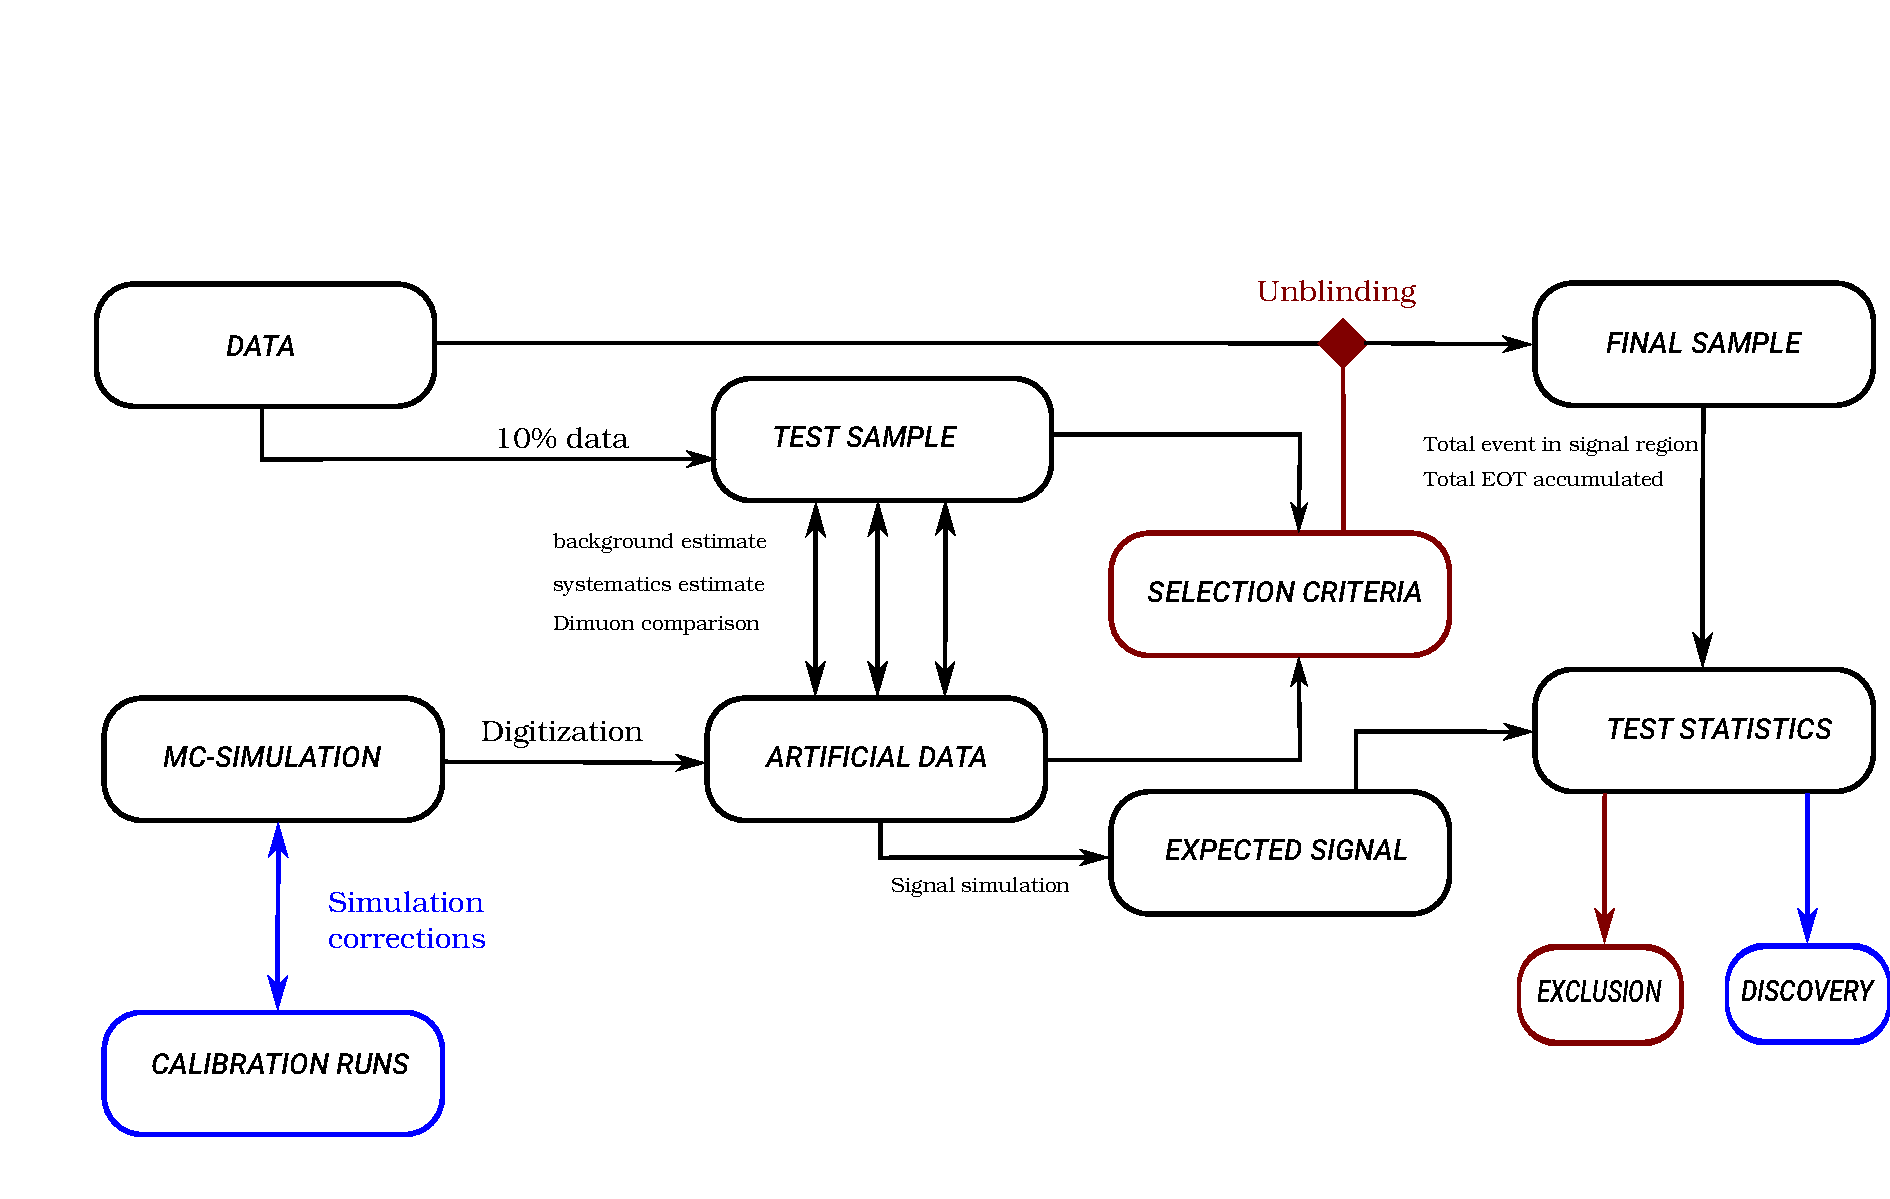
\includegraphics[scale=0.4]{\pdirthree/analysis-chart.pdf}
  \caption{Flowchart of the NA64 analysis.}
  \label{fig:analysis-chart}
\end{figure}

\section{Geant4 simulation of the experiment}
\label{ch3:sec:geant4}

The first ingredient for our analysis is Monte Carlo simulation used to reproduce the particle interactions in our setup. This task can be divided into three subtasks:

\begin{enumerate}
\item A code to simulate particle interactions inside the NA64 setup.
\item A code that describes in detail the physics of $A'$.  
\item A code to reproduce the detector response in our setup.  
\end{enumerate}

The first task is handled by the Geant4 library\cite{AGOSTINELLI2003250}. Geant4 software includes facilities to handle the geometry description, particle tracking, and run management. To produce a simulation, the end-user must provide an accurate description of the setup, a list of the interactions that need to be simulated, and the description of the primary particle, in terms of particle type\footnote{For a list of available particle and the explanation of the numbering scheme, see \cite{geant4-pdg}}, initial momentum and initial location.

The setup is described using different C++ classes to detail the precise geometry of each detector. To each geometry, a logical volume is assigned, which details the property of the geometrical object. In most cases, this means the atomic number Z, the mass number A, and the density of the material. These properties were taken from the NIST database \cite{nist-database} unless more reliable information (coming from example from the manufacturer of the detector) was available. In some cases, for example to simulate the vacuum and the gas detectors, pressure and temperature are also described using in-situ measurements. Finally, detectors are placed in the simulation using measurements done with a tape (with a precision $\sim$1 \si{\centi\meter}). For the trackers, an additional measurement was performed by the H4 meterology team with a precision of 0.5 \mmi \cite{meterology-measurements} later improved with an alignment procedure performed by the CORAL software \cite{ABBON2007455}. 

A physics list is then provided to simulate the relevant physics in the virtual setup. The physics list used in the simulation is the \textit{\textrm{FTFP\_BERT}} modular physics list, which is recommended for high-energy physics experiments \cite{ALLISON2016186}. This physics list combines an excellent description of electromagnetic physics and a description of the inelastic hadron-nucleus processes based on the Fritiof Parton Model (FTF) \cite{Uzhinsky:2013hea}, Bertini intranuclear cascade \cite{Heikkinen:2003sc} and Precompound models \cite{Apostolakis:2009zz}. Because of the absence of a precise theory of QCD at low energy, the description of the inelastic scattering for hadrons can still be problematic and a cause of systematic errors in the experiment. This problem is addressed by correcting the model using data from the calibration run, as detailed in Appendix.\ref{appC:sec:ftfp-modifications}.

Next we add the $\DM$ physics description to Geant4. This is currently done by an additional C++ code that describes Dark Matter in a modular way. This allows for the description of many Dark Matter candidates inside the same framework. The code performs the following tasks:

\begin{enumerate}
\item Compute the total cross-section of $\DM$ emission as a function of the properties of the target nucleus (namely Z, A, and density $\rho$) and the primary energy.
\item Decide for each step in the Geant4 simulation if the $\DM$ is emitted.
\item Sample the energy and angle of the final state.
\item Compute the decay time in the laboratory system if the model predicts a visible decay and pass the information to Geant4.
\end{enumerate}

An instance of the Dark Matter class is called at the start of each run, initialized with specific parameters of $\epsilon$ and $m_{\DM}$. The method of the class is then called at each step involving\footnote{In some cases this is called also for $\mu^-$/$\mu^+$ if the interaction is possible. In Sec.\ref{ch5:sec:muon-mode-setup} a setup to probe models with such interaction will be presented.} an $e^-$/$e^+$ to calculate the total cross-section and to decide if emission is performed. After that, energy and angle are sampled using a distribution $E_{\DM}(E_{e^-}, \theta_{\DM})$. In the case of the invisible mode, the energy of $\DM$ is subtracted to the particle who emitted it and its momentum recalculated. No new particle is created inside the simulation, as the NA64 experiment assumes the decay product $\dmchi$ to punch-through the setup with no further interaction. In the case of the visible mode, the decay length of $\DM$ is computed as a function of its energy, mass $m_{\DM}$ and coupling $\epsilon$. A $\ee$ pair is created inside the decay volume by sampling the corresponding decay distribution in that region. A weight corresponding to the probability of $\DM$ to decay inside the fiducial volume is saved as meta-information of the event and later used to correct the signal yield.
The differential cross-section and precise energy spectrum of $\DM$ were initially calculated using the IWW-approximation described in Sec.\ref{ch1:sec:dm-u1model}. In our new analyses, this estimate was improved using a complete tree-level calculation of the cross-section, shown in Fig.\ref{fig:dm-iww-tl}. This correction decreased the expected signal yield for mass larger than 10 MeV but increased it for mass smaller than 5 MeV \cite{DMsimulation}.

\begin{figure}[htb!]
  \centering
  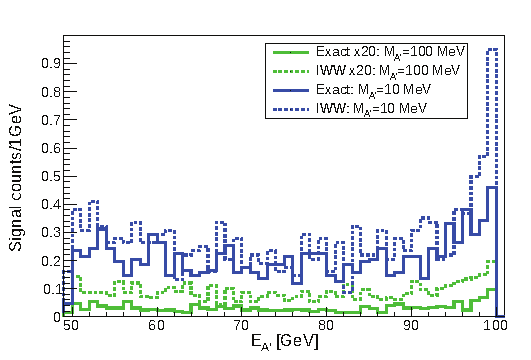
\includegraphics[width=\textwidth]{\pdirthree/DM-cs.pdf}
  \caption[IWW vs tree-level energy spectra]{Comparison of the energy spectrum of the emitted $\DM$ for a dark photon mass of 100 \mev and 10 \mev. The spectra are calculated using the IWW approximation (dotted line) and an exact tree-level calculation (continuous line) \cite{DMsimulation}.}
  \label{fig:dm-iww-tl}
\end{figure}


Finally, a biasing system was added to the code to increase the cross-section artificially. This is required to simulate efficiently the signal without the need of extremely large simulations. A correction factor $N_{norm}(\epsilon_{bias},m_{\DM})$ is calculated by the code and saved as metadata in the output. This factor is then used in the analysis of the simulations to correct for the artificial increase of the $e^- Z \to e^- Z \DM$ cross-section. The number of $\DM$ simulated scales linearly with $N_{norm}$, allowing a quick correction of the signal yield. The most relevant number for this is the expected number of $\DM$ produced normalized to the total EOTs, which we will call $\dmpereot$. This can be calculated simply from the output of the simulation using the following equation:

\begin{equation}
  \label{eq:1}
  \dmpereot = \frac{N_{norm}}{N} \times \sum^{n=N}_{i=0} \omega_i
\end{equation}

Where $N$ is the total number of events simulated, and $\omega_i$ is the weight associated with an event. For an event without $\DM$ production or that did not pass the selection criteria, this weight is zero. Else, the weight assumes a value between 0 and 1, which corresponds to the probability of $\DM$ to decay in the fiducial volume. For an invisible decay, the number is always 1, since missing energy will always be present if the events pass all selection criteria. For the case of the visible mode, the number is set to the probability of $\DM$ to decay inside the fiducial volume mentioned back in chapter \ref{chapter1}. This corresponds to the integral of the decay spectrum between the last layer of the WCAL and the scintillator (S$_4$) placed at the end of the vacuum tube.

The final ingredient to start the simulation is an input particle to start the whole machinery. This is done using electron and hadron calibration runs to extract a reliable beam profile. Hadron and electron beams are quite different from each other\footnote{This feature can also be used to cross-check the contamination of each of them, see Sec.\ref{ch3:sec:dimuons}}. For the case of hadrons, the beam is parametrized as an ellipse, with total width in the X-direction of 14.5 $\mmi$ and 6 $\mmi$ in the Y-direction\footnote{X being the coordinate aligned with the direction of the bending inside the magnetic field}. In the case of electrons, the parameterization use a 2D Gaussian distribution with $\sigma_x$=4.13 $\mmi$ and $\sigma_y$=1.4 $\mmi$. In both cases, the entrance angle of the particle is assumed to be uncorrelated with its initial position, and is parametrized with a Gaussian of width $\sigma_r$=0.4 \mrad. These parameters were obtained by fitting the beam profile recorded by the Micromegas in the calibration runs with a Gaussian in both projections. The fit was performed using the two Micromegas placed upstream the magnet and agreed within 5\% error.

\subsection{Reconstruction and digitization}
\label{ch3:sec:geant4-digitization}

The output of Geant4 can be divided into three different categories:

\begin{itemize}
\item Energy deposited in the active area of a scintillator counter or a calorimeter.
\item Hit information of a particle passing through the active area of a tracking chamber.
\item MC truth information regarding the event, including all the kinematics of the $\DM$ if it was emitted.
\end{itemize}

The first type is straight-forward. Each time a step is computed inside a sensitive detector, the energy deposited in the volume is added to specific counters which are saved at the end of each event. At this point, some detector effects are already accounted for. Only the energy in the active part of each calorimeter is recorded, and the total sum of the energy deposited is corrected using a calibration constant which corrects the energy output as it is done in the data for sampling calorimeters. Additionally, Birks law \cite{NYIBULE2014141} is implemented in the HCAL to correct for the propagation of optical photon in the WLS until the PMTs, using an attenuation length of 30 \si{\centi\meter}. This is to correct for the different light yields between $\pi^-$ and $\mu^-$, since in the case of $\mu^-$ the energy is deposited the full length of the detector evenly.

To reproduce tracking detectors, every time a particle crosses the gas volume of a gas chamber, multiple pieces of information are saved:

\begin{itemize}
\item x-y-z position of the particle at the beginning of the step.
\item The energy of the particle responsible for the hit.  
\item The energy deposited in the gas during the step.
\item The PDG number of the particle \cite{particle-numbering-scheme}.
\end{itemize}

These data define a structure called \textit{MChit}, which is used by the reconstruction algorithm to reproduce both hits and tracks in the same format of the data. This algorithm was developed during my thesis to improve the Digitization procedure. It works as follow:
\begin{enumerate}

\item Hits with an energy deposited in the volume smaller than the minimum amount to start the ionization inside the gas are removed. Practically, this threshold was set to 2 keV based on previous studies performed for MM \cite{IGUAZ20121079}. A similar value is assumed for the GEM detector as well.
\item Multiple \textit{MChit} are merged if they are found to be closer than a fixed distance. This distance is conservatively set to be 2 $\mmi$  for MM and 1.75 $\mmi$  for GEM. The new x-y position of the hit is computed using the weighted average of each hit position, where the weight is defined by the energy deposited inside the gas.
\item The x-y coordinates of the hits are transformed into the plane of the detectors using a simple matrix multiplication $u_{hit} = M_{uv}(\theta_{uv}) \cdot v_{hit}$ where $u_{hit}$ is the hit position in the detector coordinate system and $v_{hit}$ is the same vector expressed in the laboratory system. The Matrix $M_{uv}(\theta_{uv})$ is the rotation matrix of the $O(2)$ group where $\theta_{uv}$ is the angle between the axis of the detector and the axis of the laboratory system.
\item Each coordinate on the detector plane is treated separately. To reproduce the genetic multiplexing of the MM, each physical strip is mapped to its corresponding channels, and a 64-dimension vector is obtained as output. Noise is also added to each channel using the same pedestal measured in the sparse mode of the APV chips.
\item  The charge vector is used as input for the same clusterization procedure used for the data. In the MM detector, the clusterization is fully reproduced. the physical cluster is parametrized by a Gaussian, and the charge is distributed on the physical strips starting from the hit center. The total charge of the cluster is decided starting from the total energy deposited in the gas volume and converted into ADC counts. The constant of conversion is computed using the data of the electron calibration runs. The procedure for the GEM is more direct and only involves the smearing of the initial true hit position using a Gaussian distribution with a width corresponding to the hit resolution of the GEM detectors. This was estimated to be $\sigma_{GEM} \approx 80$ $\mum$ using the Three Layer Method \cite{Bortfeldt:2014vvt}.
\item After the clusterization is performed, two set $X_n$ and $Y_n$ of positions are extracted from the two planes and combined\footnote{In the most common case of just a single primary present upstream the ECAL, this association is trivial, since only one hit per plane is present.} in the set of hit candidates $(X;Y)_n$. A hit number per plane larger than five, other than being rare ($\lesssim$0.1\%), is not relevant for $\DM$ searches and hence rejected in the reconstruction. The hits candidates are then used as input of the tracking or vertexing procedure. The total momentum of a track is calculated from the displacement after passing through the magnetic field of the MBPL (see Appendix.\ref{AppendixD}). The vertex reconstruction is more involved but starts from the same input. The procedure is described more in detail in Sec.\ref{ch3:sec:vis-mode-tracking}.
\end{enumerate}

Completed the procedure, these quantities are saved in a tree structure implemented in ROOT \cite{root} that is equivalent to the one used for the data. A shower profile analysis is also performed at this step (see Sec.\ref{ch3:sec:bkg-ecal-profile}) and added to the tree. This design allows using the same analysis to study MC and data without the need of changing the code.

\section{Monte Carlo validation using $\gamma + Z \rightarrow \mu^+ \mu^-$ events}
\label{ch3:sec:dimuons}

The $\emu$ interaction consists of the rare production of a $\mu^+mu^-$ inside an em-shower after an incoming photon interacts with a target nucleus. The process of pair production is equivalent for all charged leptons (e,$\mu$,$\tau$) and has a cross-section in the order of $\sigma_{pair} \sim 4Z^2\alpha r^2_c$. Compared to the more frequent $\ee$ production, this interaction is suppressed by a factor ($m_e$/$m_{\mu}$)$^2$ = 2.34 $\times 10^{-5}$ because of the larger muon mass. This process is used both to validate the MC simulation and estimate the systematics of the experiment, as it shares many similarities to the signal under study:

\begin{enumerate}
\item Rare process produced inside an em-shower.
\item In first approximation, it can be computed inside the QED framework, hence with high precision.
\item The process penetrates very efficiently both the target and the HCAL modules. Each $\mu^{\pm}$ loses an energy $<250$\si{\mega\electronvolt} after its passage through the target, and $\sim$1.3 $\gev$ for each HCAL module encountered. 
\item While the energy spectrum of the emitted $\mu^+\mu^-$ is not equivalent to the one of $\DM$ \cite{dimuon-mc}, it spans the same energy region relevant for the $\DM$ signal.
%Hence, a comparison between MC and data for dimuons is an excellent test for the reliability of the MC.
\end{enumerate}

Additionally, because of the double MIP signature that the $\emu$ interaction leaves inside the VETO and the HCALs, this interaction can be easily distinguished from a signal event. The possibility of the leakage in the signal region was computed for both invisible and visible mode and was found not to be a relevant background (see for example Sec.\ref{ch3:sec:bkg:vis:elec}).

In Geant4, the process is described starting from the formula \cite{dimuon-mc}:

\begin{equation}
  \label{eq:sigma-dimuon}
  \sigma_{tot}^{\gamma \to \mu^+ \mu^-}(E_{\gamma}) = 4\alpha Z^2 r^2_c\int^{x_{max}}_{x_{min}} \left(1 - \frac{4}{3}x_+x_- \right) \log{W}dx_+
\end{equation}

Where $x_+$ the fraction of energy of the original $\gamma$ being transferred to the $\mu^+$ and $W$ is a function of $x_+$,$E_{\gamma}$, and the Z, A of the element, which also takes into account both the atomic-screening using the Thomas-Fermi model and the finite size of the nucleus. Numerical values for this are provided in \cite{dimuon-mc}. To increase computation speed, a parameterization of Eq.$\ref{eq:sigma-dimuon}$ is used instead, with a precision greater than 2\%. After the dimuon pair is generated, the amount of energy transferred to the $\mu^+$ is decided by sampling the differential cross section\footnote{In this case, just the argument of the integral in Eq.\ref{eq:sigma-dimuon}} and the new particles are produced in Geant4. Since the interaction is approximately elastic, the relation $E_{\gamma} = E_{\mu^+} + E_{\mu^-}$ is used for the computation.

For a comparison between data and MC, $\emu$ interaction are collected from the complete sample of data collected for both visible and invisible mode using the criteria $\SI{1.2}{\giga\electronvolt} < E_{HCAL}^{1,2,3} < \SI{6.35}{\giga\electronvolt}$ compatible with the passage of two MIPs in all HCAL modules. All selection criteria are then applied to the sample obtained, excluding energy deposited on the VETO (and W2 in the case of the visible mode). After that, the energy spectra recorded in the target is compared between data and MC. First, both samples are normalized to the same value to compare the shapes of the two spectra and check the reliability of the MC. After that, the two distributions are normalized to the number of EOT collected, the difference between the two is taken as a correction factor to the total number of EOT accumulated, as it shows some disagreement between data and MC prediction due to the systematics of the experiment \cite{na64-prd}. Correction factors can be derived from the detailed comparison of the energy deposited in the ECAL between data and MC. Each bin of the spectrum is compared and the ratio is computed using the formula:

\begin{equation}  
  \label{eq:RR-factor}
  \begin{aligned}
  &R_{data/MC} = \frac{n_i^{ECAL}}{n_{tot}^{ECAL}} \\
  &RR_i = R_{data}/R_{MC}
  \end{aligned}
\end{equation}

Inside the MC simulation, each event is weighted by the corresponding factor $RR_i$ as a function of the energy deposited in the target. Such corrections are different between runs and are mostly affected by the intensity of the beam and the variation of the trigger-threshold in the PS detector during data taking. The signal yield is reduced by 5\%-10\% after these corrections are applied. Differences in reweighting between runs collected at the same intensity are taken as systematic errors, which amount to a maximum of 7\%\footnote{The precise error has a small dependence from the $\DM$ mass, for masses of $\simeq$10 MeV this error amount to 5\% \cite{na64-prd}.}. An example of such comparison is shown in Fig.\ref{fig:dimuon-comp-invis}.

\begin{figure}[tbh!]
  \centering
  %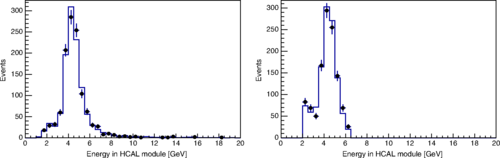
\includegraphics[width=\textwidth]{\pdirthree/dimuon-hcal-comp.png}
  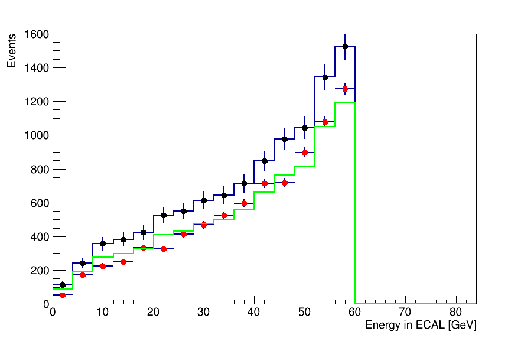
\includegraphics[width=0.45\textwidth,height=0.43\textwidth]{\pdirthree/dimuon-ecal-comp.pdf}
  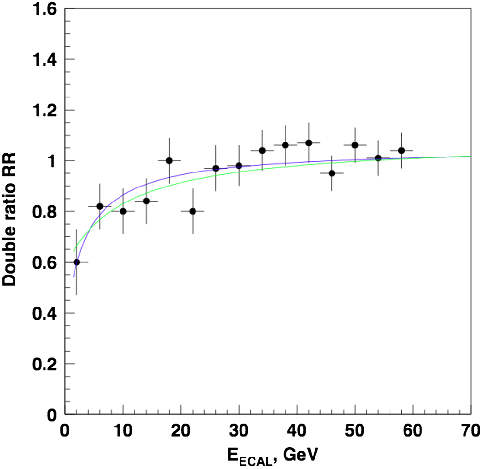
\includegraphics[width=0.45\textwidth,height=0.4\textwidth]{\pdirthree/dimuon-RR-comp.pdf}
  \caption[Dimuon spectra in ECAL for data and MC.]{Left: Distribution of energy deposited in the ECAL target by the scattered electron from the reaction $\emu$ selected from data (red dot) and MC generated event (green line). Data and MC are normalized to the same number of event. The unnormalized MC distribution is also shown with the corresponding error on the top histogram. Right: Ratio RR between MC and data efficiency of dimuon production as function of the energy deposited in the ECAL. The two color curves shows examples of empirical distribution of the values \cite{na64-prd}.}
  \label{fig:dimuon-comp-invis}
\end{figure}

\section{Background rejection methods}

Part of my work was also to improve the background condition. In this section, I will describe two methods developed during my thesis for this purpose.

The first method exploits the emission of synchrotron radiation by the electrons during their passage in the magnetic field to distinguish the ID of the incoming particle. The nature of this radiation is described more in detail in Appendix.\ref{appB:sec:sr}, together with the most relevant equations to describe its phenomenology. The method was tested using BGO crystals during the test beam performed in 2016 and resulted in a total suppression of hadrons of $\simeq 10^{-5}$ published in \cite{Depero:2017mrr}.

The second method consists of a shower profile analysis to check the compatibility of the energy deposited in each cell with the one predicted for an em-shower. A set of measurements performed using calibration runs were used to build a model to predict the energy deposit as a function of the impact point of the incoming particle extrapolated from the Micromegas.  This method was documented in an official NA64 note \cite{na64-shower-profile}, and achieved a background suppression of $\simeq 10^{-3}$.

\subsection{Heavy charged particle rejection using synchrotron radiation}
\label{ch3:sec:bkg-srd}

The rejection of the heavy charged particle is one of the main tools to reject the contamination of $\pi^-$,$K^-$, and $\mu^-$ present in the beam. The working principle of this method is simple in its approach. A particle traveling through a magnetic field will emit synchrotron radiation. With minimal assumptions, the total power after a full cycle can be calculated is the useful formula :

\begin{equation}
  \label{eq:srd-power}
  P = \frac{q^2 c}{6 \pi R^2}\frac{E^4}{m^4}
\end{equation}

Here R is the bending radius experienced from the particle when inside a magnetic field B perpendicular to its velocity. From this equation, we see that the total power scales to $P\sim E^4/m^4$. This both means that the technique is suitable for high-energy particle, as the signal will be boosted, and is useful to separate particles with large differences in the mass spectrum. The difference in mass between the electron and all other particles is so large in fact that effectively no radiation is emitted at the energy of the H4 beamline. 

Simulation of the expected SR signal was performed with the Geant 4 package\cite{ALLISON2016186,1610988,AGOSTINELLI2003250}.
The geometry of the NA64 experiment was coded in Geant 4, including the 200 $\mu$m mylar vacuum windows, the detailed composition of the trackers, scintillators and the residual gas was set at a level of $10^{-3}$ mBar as in the measurements. Saturation of BGO was taken into account using Birks' law with the constants taken from \cite{AVDEICHIKOV2002251}.

The expected SR spectra for pions and electrons with energies of 50 GeV and 100 GeV are shown in Fig. \ref{fig:SRspectrum}. The plot shows the expected dependence on the incoming electron energy in the emission spectra for the realistic experimental conditions. Moreover, the comparison between the SR spectra of pions and electrons illustrates clearly the principle of this technique that allows to discriminate between them by requiring an energy threshold in the synchrotron detector.  For pions, one can see that the probability of detecting an event with energy above 1 MeV is about $\sim 10^{-3}-10^{-4}$.
These SR-like signals originate from the interactions of the incoming pions with materials placed along the beamline. Although in first approximation the energy transfer due to ionization is in the order of few \si{\kilo\electronvolt}, rare high energy transfer is also possible. The distribution of such secondary electrons with
kinetic energy $T\gg I$, where $I$ is the mean excitation energy of the
atom/molecule, for a particle with velocity $\beta=v/c$ and charge $z$
passing through a material with atomic number $Z$, mass number $A$ and
thickness $dx$ is described by \cite{review-particle-physics}:
\begin{equation}
\frac{d^2N}{dTdx} = \frac{1}{2}K z^2 \frac{Z}{A}
\frac{1}{\beta^2}\frac{F(T)}{T^2}
\label{eqn:knock-on}
\end{equation}
The constant $K$ is defined as $K=4\pi N_A r_e^2 m_e c^2$ where N$_A$ is
the Avogadro's number, $r_e$ is the classical electron radius and $m_e$
the electron mass.
$F(T)$ is a spin-dependent factor, which in our case for $T \ll W_{max}$
is very close to unity. W$_{max}$ is the maximal energy transfer in a single collision to the
electron:
\begin{equation}
W_{max} = \frac{2m_e c^2 \beta^2 \gamma^2}{1+ 2\gamma m_e/M+(m_e/M)^2}
\end{equation}
For a $\pi^-$ at 100 GeV, $W_{max}$ is roughly 1 GeV which
covers completely the energy range where synchrotron radiation is
emitted. Eq.\ref{eqn:knock-on} is valid in the range $I\ll T \leq W_{max}$.
 \par 
Furthermore, Geant 4 reproduces the critical energy $E_c$ which divides the spectrum into two parts of equal power is:
\begin{equation}
E_c = \frac{3 \hbar c \gamma^3}{2R}
\end{equation}
with the reduced Plank constant $\hbar$ and the bending radius $R$. 
 For 100 GeV electrons in the  $B=1.7$ T bending field this corresponds to $E_c\sim$11.35 $\mev$. The expected mean energy of a synchrotron photon $E_m=E_c/\pi\simeq 3.6$ $\mev$ is in very good agreement with simulation. The number of photons emitted per revolution in this energy range in the field of \SI{7}{\tesla\meter} is defined as:
\begin{equation}
N_\gamma = \frac{5 \pi \alpha}{\sqrt{3}}\gamma
\end{equation}
where $\alpha$ is the fine structure constant. 
By scaling this equation for the fraction of the circle where the particles are inside the magnetic field, one obtains a mean number of emitted photon of about 24.
The SRD geometrical acceptance is about one third,  thus one can estimate that the sum of deposited energy is approximately 29.35 $\mev$ in good agreement with the results of the simulation as shown in Fig.\ref{fig:SRspectrum}. 
 
\begin{figure}[htb!]
\centering
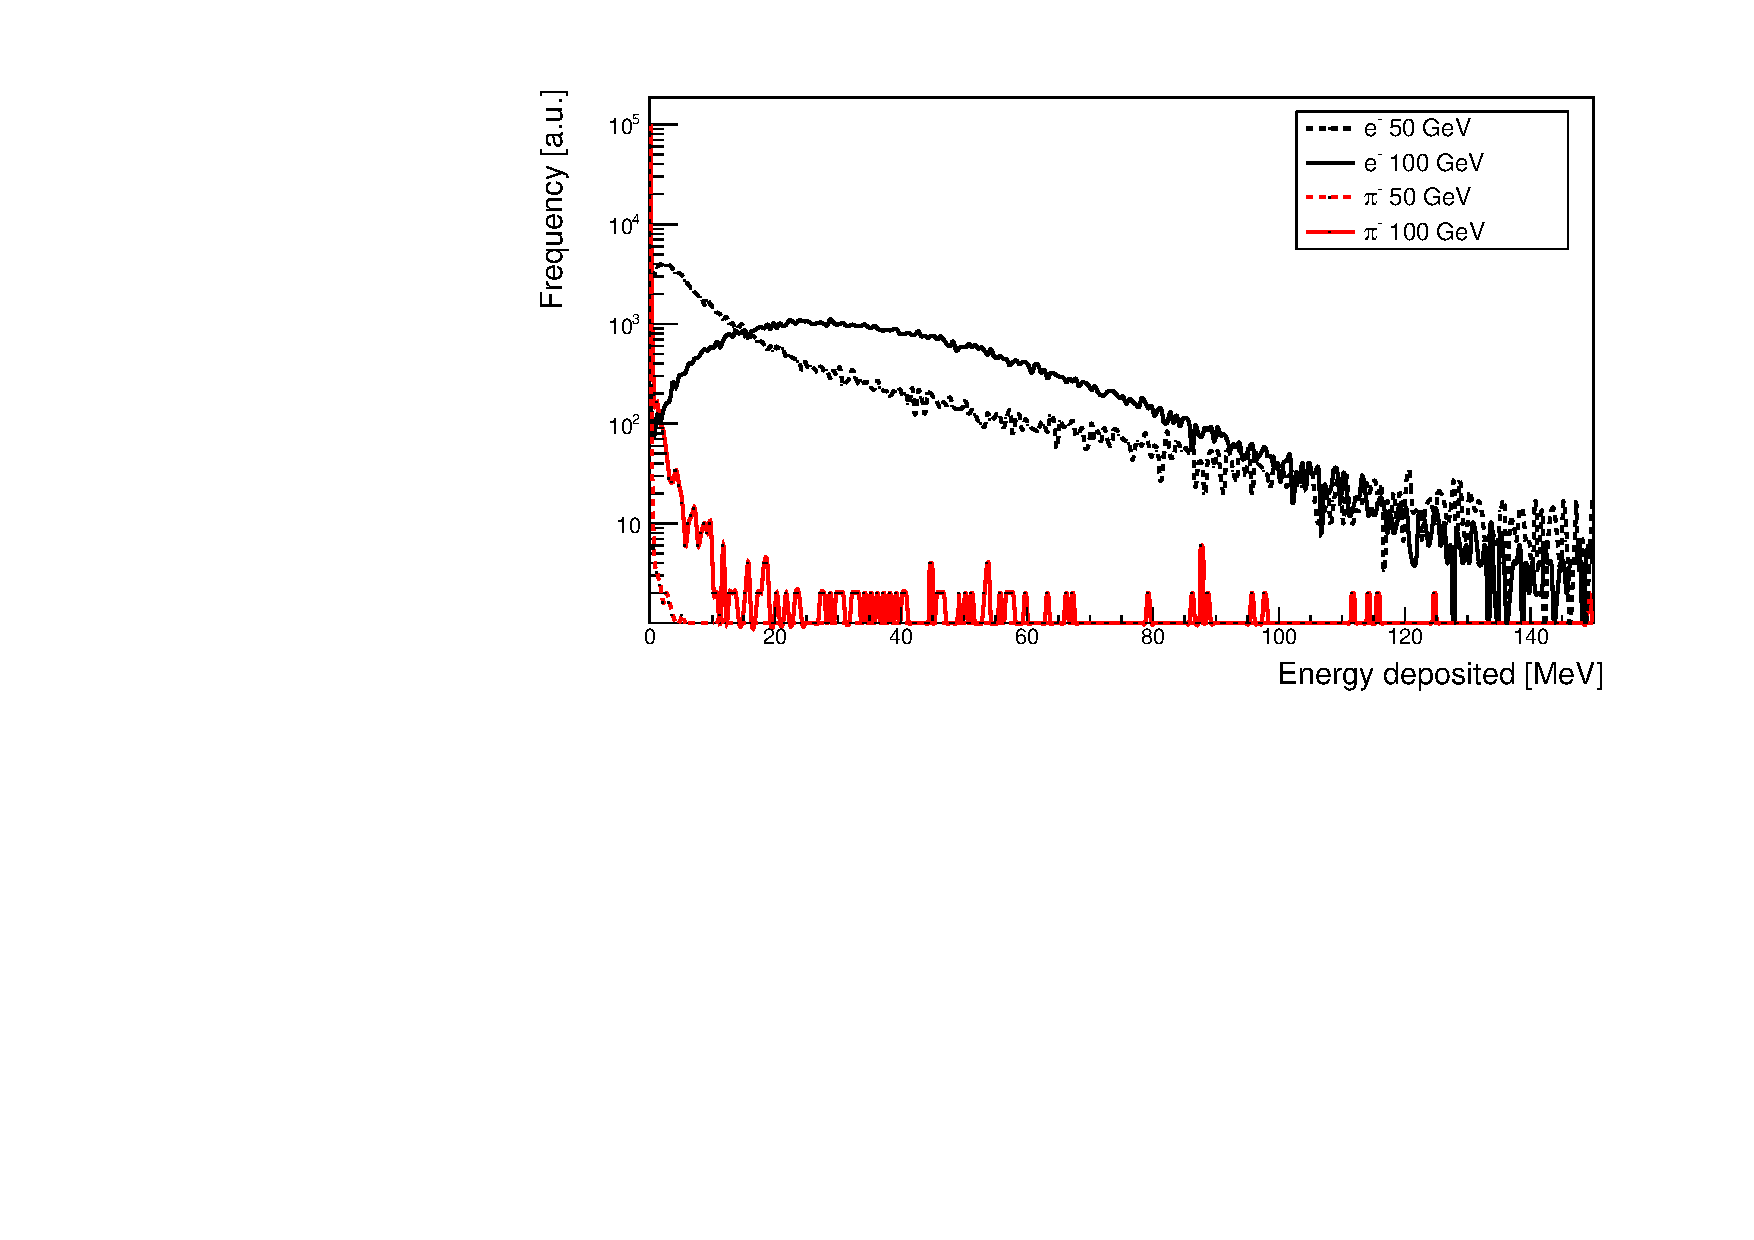
\includegraphics[width=1.\textwidth]{\pdirthree/comp_spectra.pdf}
\caption[SR spectrum for different energy detected in the SRD]{Result of the Geant 4 simulation for the energy detected by the SR detector for 50/100 GeV e$^-$(black dashed/solid line) and 50/100 GeV $\pi^-$ (red dashed/solid line).}
\label{fig:SRspectrum}
\end{figure}

The SRD detector was tested during the NA64 test beam run in July 2016. The two BGO rows are parallel to the primary beam direction as shown in Fig.\ref{fig:newgeo}. The dipole magnets installed in series produce a total integrated magnetic field of 7 \si{\tesla\meter} \cite{Banerjee:2016tad} resulting in a nominal displacement for the incoming electrons at the SRD/ECAL positions of 31/34 cm from the undeflected beam axis. The SRD was placed between the undeflected and the deflected beam axis at a distance of approximately 9 cm from both (Fig.\ref{fig:newgeo}). This separation minimises the possibility for Bremsstrahlung photons and neutral particles produced by interactions of the beam particle with materials upstream and for particles in the beam halo to hit the SRD. In fact, such interactions result in the saturation of the SRD with a significant loss of efficiency due to the long decay time of the BGOs.

%The expected Landau distribution of energy deposits was fit to the data to find the mean peak position to extract the calibration constant. 

The two crystals facing the beam (labeled 3 and 7 in Fig. \ref{fig:newgeo}) detect most of the energy emitted by synchrotron radiation. We will refer to those as SRD BGO. The remaining six crystals are used to detect events with high energy deposition in the SRD. In particular the last two crystals of each row (labeled 0 and 4 in Fig. \ref{fig:newgeo}) detect some energy only in the case of very energetic Bremsstrahlung events and thus can be used as a veto (see Fig.\ref{fig:newgeo}). The six crystals after the SRD BGOs act also as a shield from backscattering particles coming from the ECAL suppressing pions by an additional order of magnitude. Finally in this geometry it is possible to use the coincidence of the two SRD BGO crystals to improve the tagging of synchrotron photons by rejecting knock-on electrons produced by incoming pions. In fact synchrotron radiation has an homogeneous spectrum in the whole arc described by the primary and deflected beam and thus a signal is detected in both SRD BGO. On the contrary, electrons generated by a $\pi^-$ undergoing ionisation will mostly leave energy only in a single crystal as illustrated in Fig. \ref{fig:newgeo}. 
With the requirement of detecting in both SRD BGOs an energy deposition above a 1 MeV the suppression factor is improved up to a level of $10^{-5}$.



\begin{figure}[htb!]
  \centering
  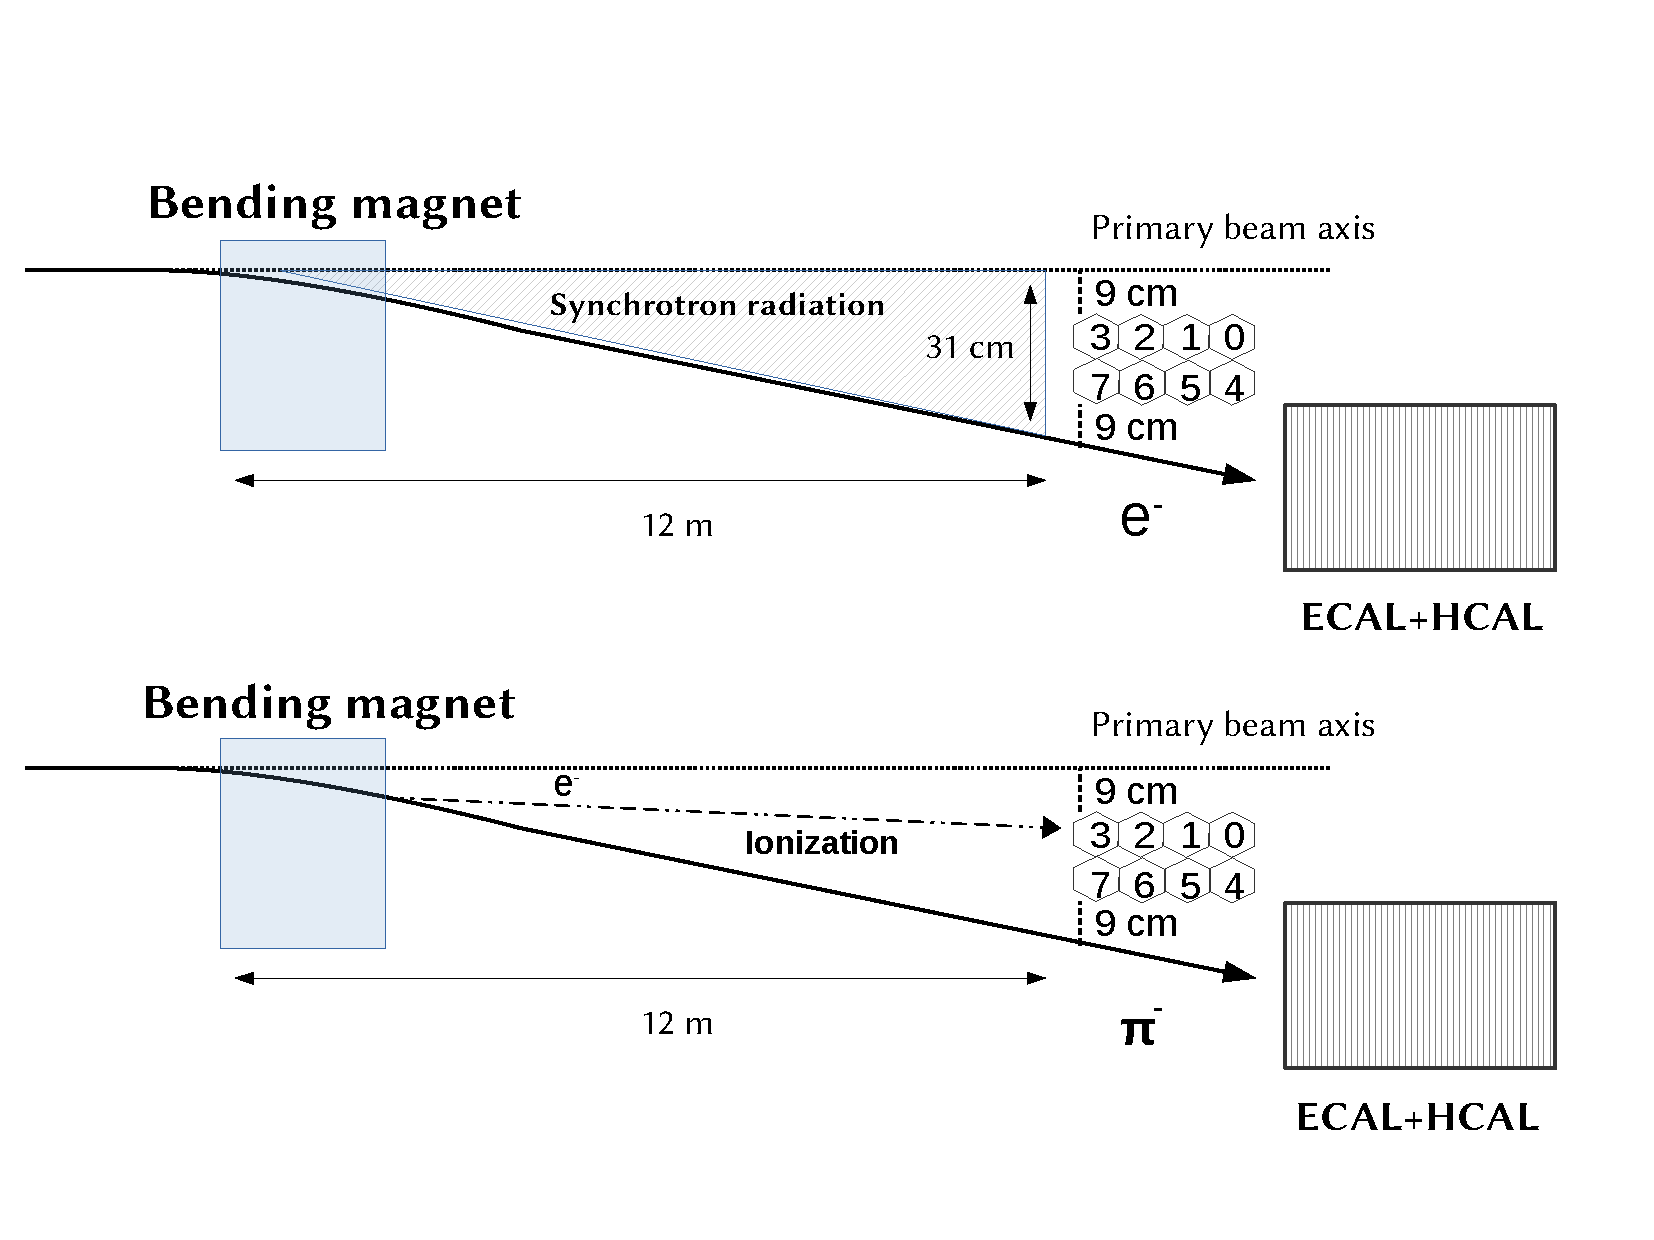
\includegraphics[width=.9\textwidth]{\pdirthree/sketch.pdf}
  \caption[Geometry of the BGO crystals]{Geometry of the BGO crystals. Crystals 7,3 (SRD BGO) collect most of the synchrotron radiation spectrum. Crystals 4,0 (VETO BGO) on the other hand are effected only in case of a high energy event and are thus used as a veto. The remaining crystals serve as a shield for the SRD from backscattering particles coming from the ECAL. Top: illustration of event leaving a SR signal in the SRD. Bottom: illustration of a SR- like signal in the SRD for a knock-on electron produced by pions.}
\label{fig:newgeo}
\end{figure}

Data with a 100 GeV $\pi^-$ beam were taken to have a direct measurement of the suppression factor achievable through synchrotron radiation measurements. The beam intensity was 5.3$\times 10^4$ particles per spill. The additional requirement of an energy deposition below 60 GeV in the ECAL was applied in order to completely reject electrons from the $\pi^-$ sample of $\sim 10^5$ collected events.

For the 100 GeV electron beam run, a total of 220 spills were recorded with an intensity of 3.4$\times 10^5$/spill. 
The same trigger used in the pion run was used for the electron data.
In this case though, in order to reduce the pion contamination events with a total energy deposition in ECAL + HCAL above 90 GeV but with less than 20 GeV energy in the HCAL were used.  


The energy spectra recorded by the SRD BGO with electrons and pions are shown in Fig.\ref{fig:comp_spectra}. The SR spectra obtained with the electron beam are used to perform the BGO calibration by comparison with the simulation. With this method a very good agreement of data and MC is achieved (see plot on the left of Fig.\ref{fig:comp_spectra}). As a cross check, using the obtained calibration constants, the data from the pion beam impinging directly on the SRD are fitted with a Landau distribution. The obtained peak position of 60 MeV is in good agreement with the prediction of the MC. 

Time coincidence of signals above the energy threshold of 1 MeV from both SRD counters is required and high energy Bremsstrahlung events are removed using the veto BGO.
The suppression of synchrotron radiation emission detected for pions compared to electrons is clearly visible by comparing the two plots. For the electron spectrum, a 1\% pileup beam events have been added to the simulation as predicted for the given spill intensity and with the known decay time of BGOs.  Both spectra are in very good agreement with the simulation.

\begin{figure}[htb!]
  \centering
  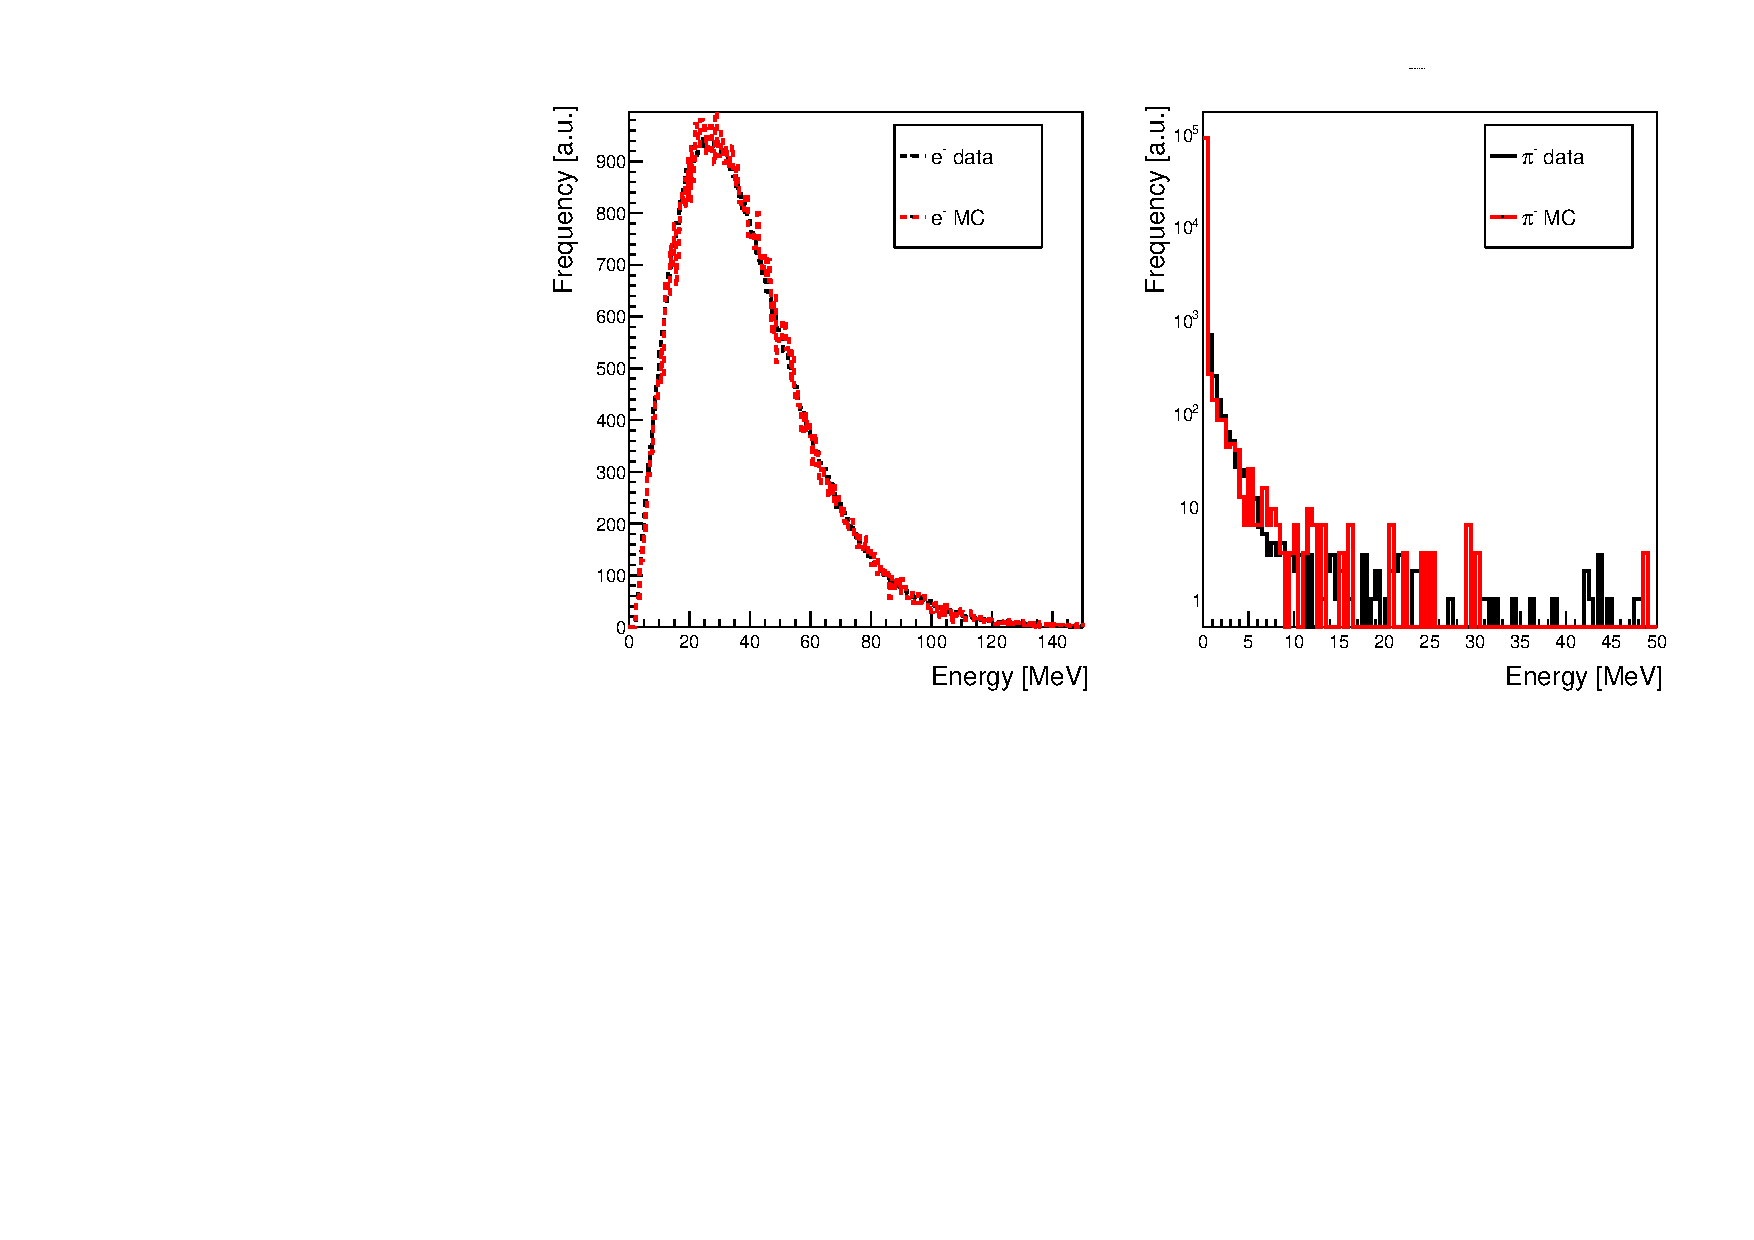
\includegraphics[width=1.\textwidth]{\pdirthree/spectra_tot.pdf}
  \caption[SRD comparison between data and MC]{Comparison between data and simulation (MC) of the synchrotron radiation spectrum detected for 100 GeV electrons (left) and pions (right). }
  \label{fig:comp_spectra}
\end{figure} 

\begin{figure}[htb!]
  \centering
  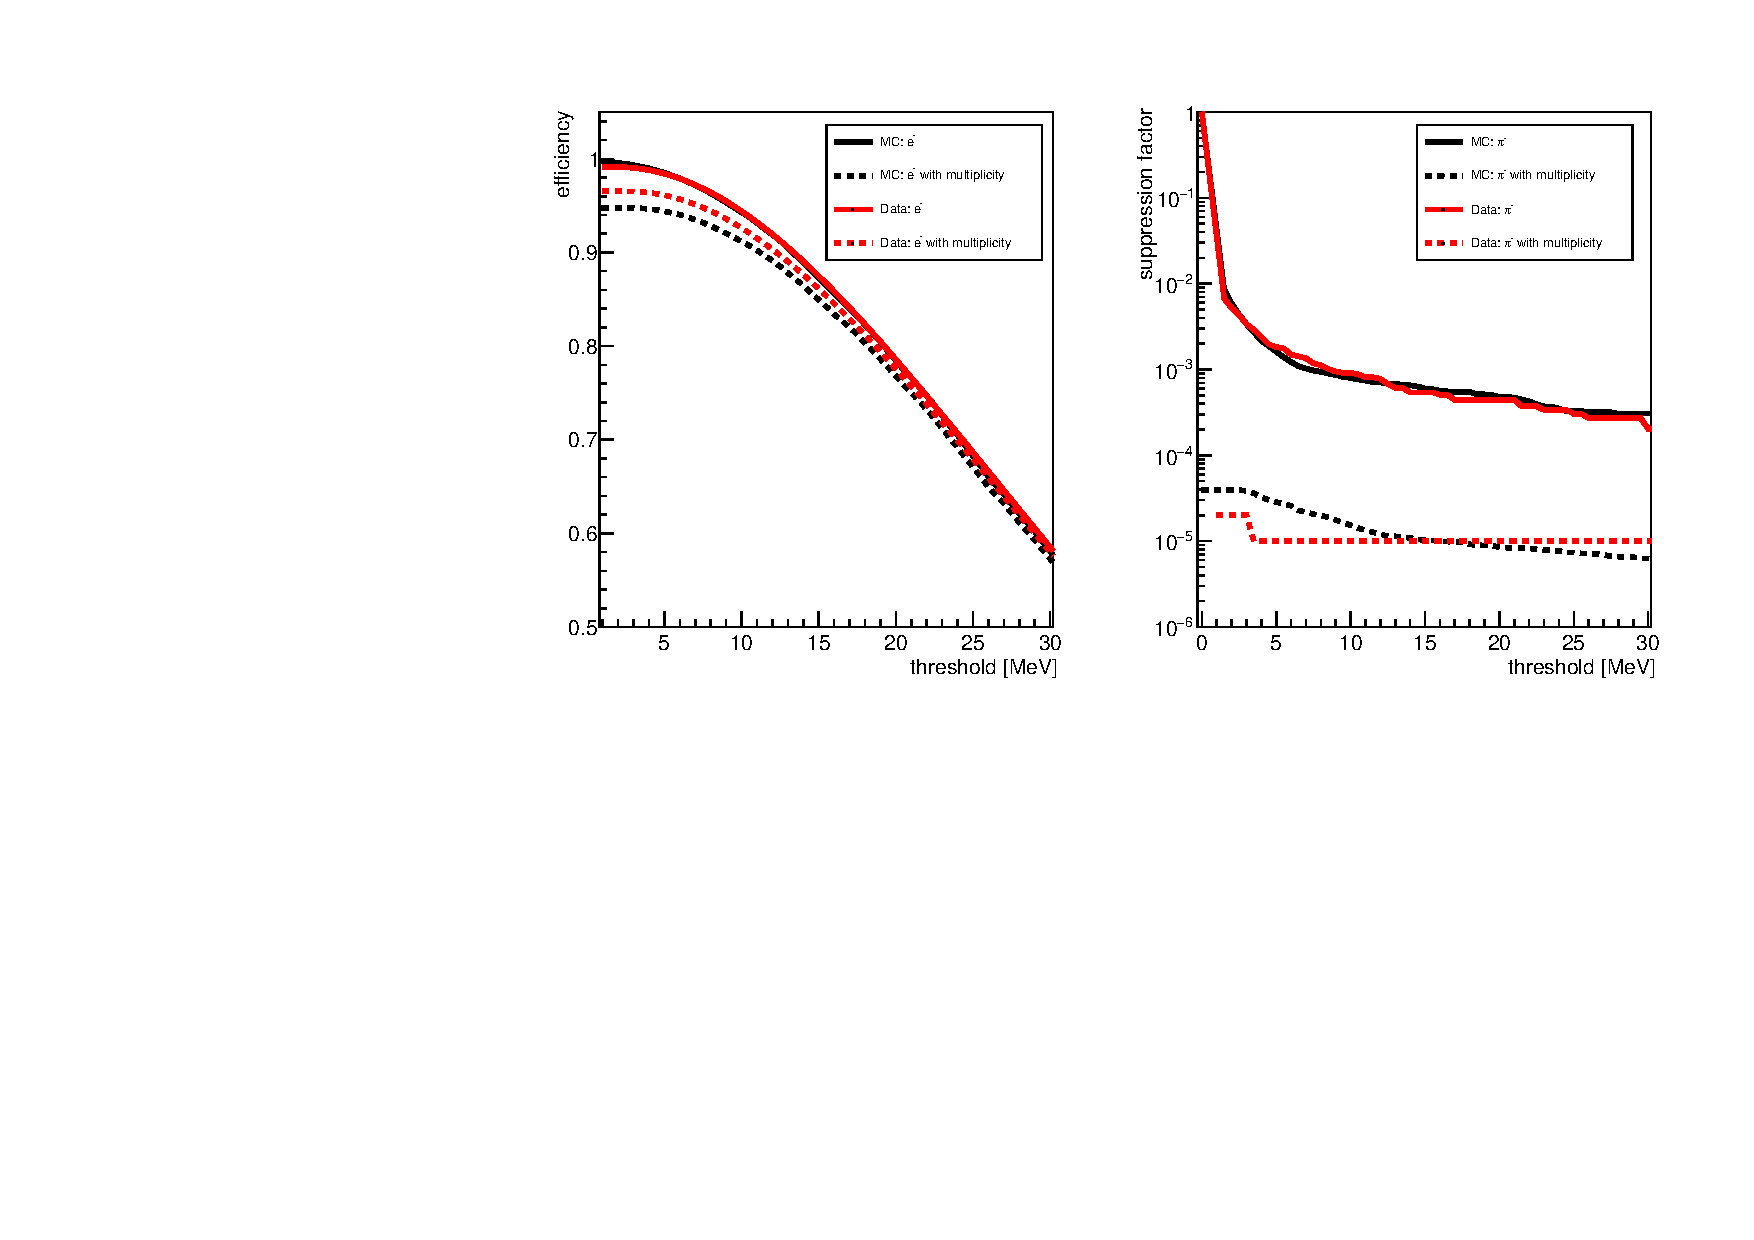
\includegraphics[width=1.\textwidth]{\pdirthree/sup_mult.pdf}
  \caption[efficiency and rejection power of the SRD cut]{Left: Comparison between data and simulation (MC) for electrons of the efficiency as a function of threshold set on the total energy deposited in the SRD BGO and for the requirement that this is deposited in each single crystal (multiplicity). Right: Comparison between data and simulation for pions and electrons of the suppression factor as a function of the threshold set on the total energy deposited in the SRD BGO and for the multiplicity requirement.}
  \label{fig:sup_mult}
\end{figure}

The efficiency for the electrons and the suppression factor for the pions are plotted in Fig. \ref{fig:sup_mult} as a function of the threshold on the energy deposited in the SRD. We distinguish between two cases:
\begin{enumerate}
\item The threshold is set on the total energy deposited in the SRD.
\item Both SRD signals have to be in-time and above the threshold of 1 MeV (multiplicity requirement).
\end{enumerate}
One can see that applying the criterion 2) the efficiency only decreases slightly compared to 1), while the suppression factor for pions is dramatically increased (by two orders of magnitude).
This is because the SR-like signal generated from secondary electrons will leave a signal only in one of the two BGOs while the SR from electrons is spread out uniformly.
This is also underlined by Table  \ref{tab:hits} where the fraction of events with different hit multiplicity in the SRD BGO for both pion and electron runs are reported.

\begin{table}[hbt!]
\begin{center}
\begin{tabular}{cccc}
Events hit multiplicity  (\%) & 0 BGO  & 1 BGO & 2 BGOs\\
\hline
Pions & $98.77$ & $1.21$ & $1.4\times10^{-3}$  \\
Electrons & $2.4\times10^{-1}$  & $2.60$ & $97.37$ \\
\end{tabular}
\end{center}
\caption[Fraction of pion and electron events for different hit multiplicity in the SRD from the data]{Fraction of pion and electron events for different hit multiplicity in the SRD from the data.}
\label{tab:hits}

\end{table}

\subsection{Hadron rejection using electromagnetic shower profile}
\label{ch3:sec:bkg-ecal-profile}

The transversal segmentation of the ECAL offers another tools for hadron rejection. The idea is to discriminate between an em-shower profile and an hadronic one  using a $\chi^2$-test. A shower profile database can be built by correlating the hit position (x,y) on the ECAL with the fraction of energy deposited in each ECAL cell. The method used to build this database is detailed in Appendix.\ref{Appb:sec:make_profile}. A predicted value of energy deposited in each ECAL cell is extracted and compared to the one measured in the event. The compatibility between the predicted profile and the measured one can be tested using the $\chi^2$-distribution:

\begin{equation}
  \chi^2 = \sum^{9,36}_i \left(\frac{E_{pred}^i(x_{hit},y_{hit})-E_{mes}^i}{\sigma^{i}_{pred}(x_{hit},y_{hit})}\right)^2
  \label{eqn:chi}
\end{equation}


\begin{description}
\item[$E_{pred}^i$]: is the energy predicted by the profile of cell
  $i$
\item[$E_{mes}^i$]: is the energy measured in the cell $i$
\item[$x_{hit},y_{hit}$]: coordinates of the hit position of the
  particle in the ECAL plane
\item [$\sigma^{i}_{pred}$]: error estimated for the predicted energy
  in cell $i$
\end{description}


Two different summation indexes are used for the two different cases
where only the cells surrounding the central one hit by the beam are
used for the test (total of 9 cells) and the case where all the cells
are used (total of 36, see Fig.\ref{fig:ecal_example}).

\begin{figure}[h!]
  \begin{center}
    \includegraphics[scale=0.47,page=4]{\pdirthree/ecal_example.pdf}
  \end{center}
  \caption[ECAL sketch]{sketch of the 36 cells of the ECAL. The central cell 3X3
    were the beam is directed is plotted in red, while the cells
    surrounding it are plotted in green. On the bottom-right an
    example of how a profile for a cell looks like in the MC.}
  \label{fig:ecal_example}
\end{figure}

To test the rejection power and the efficiency of the
method the algorithm described above was used for 3 type of samples\footnote{The database was generated using the electron  calibration runs 2363, 2182, 2410, 2406, 2438. A complete description of such runs can be found in \cite{na64-runs}. }:
\begin{itemize}
\item $\simeq$1.2$\times 10^{6}$ events acquired with an electron calibration run\footnote{run 2363}.
\item $\simeq$5$\times 10^{5}$ events acquired with an hadron calibration run\footnote{run 2204}.
\item $\simeq$8$\times 10^{5}$ events acquired using physical trigger at maximum H4 beam intensity.\footnote{run 2241, corresponding EOT before trigger suppression $\simeq 4 \times 10^{8}$}
\end{itemize}

The comparison of the normalized $\chi^2$-distribution between
electron and hadrons calibration runs using information from all 36
cells is shown in Fig.\ref{fig:chi2}. Note that electrons reproduce
the expected shape of a $\chi^2$-distribution while for hadrons we
observe a displaced one incompatible with the one produced by
electrons.  The rejection and efficiency of a cut
$\chi^2 < \chi^2_{cut}$ are shown in Fig.\ref{fig:eff}. For
a benchmark cut $\chi^2_{cut} = 2$ the efficiency calculated in run 2363
was $\sim 0.94$ with a rejection factor of $1.2\times 10^{-3}$
extracted from the hadron run 2204.

Using the 9 central cells (Fig.\ref{fig:ecal_example}) appears to shift the distribution
to the left and reduce its spread ( Fig.\ref{fig:chi}) due to the
smaller number of degrees of freedom, the two methods have overall
comparable efficiency as can be seen in Fig.\ref{fig:eff} but smaller
rejection power when the benchmark cut is applied.  For $\chi^2_{cut}=$2, the efficiency measured using only
central cells was of $\sim 0.93$\ and a rejection factor of $3.1\times 10^{-3}$.


\begin{figure}[h!]
  \begin{center}
    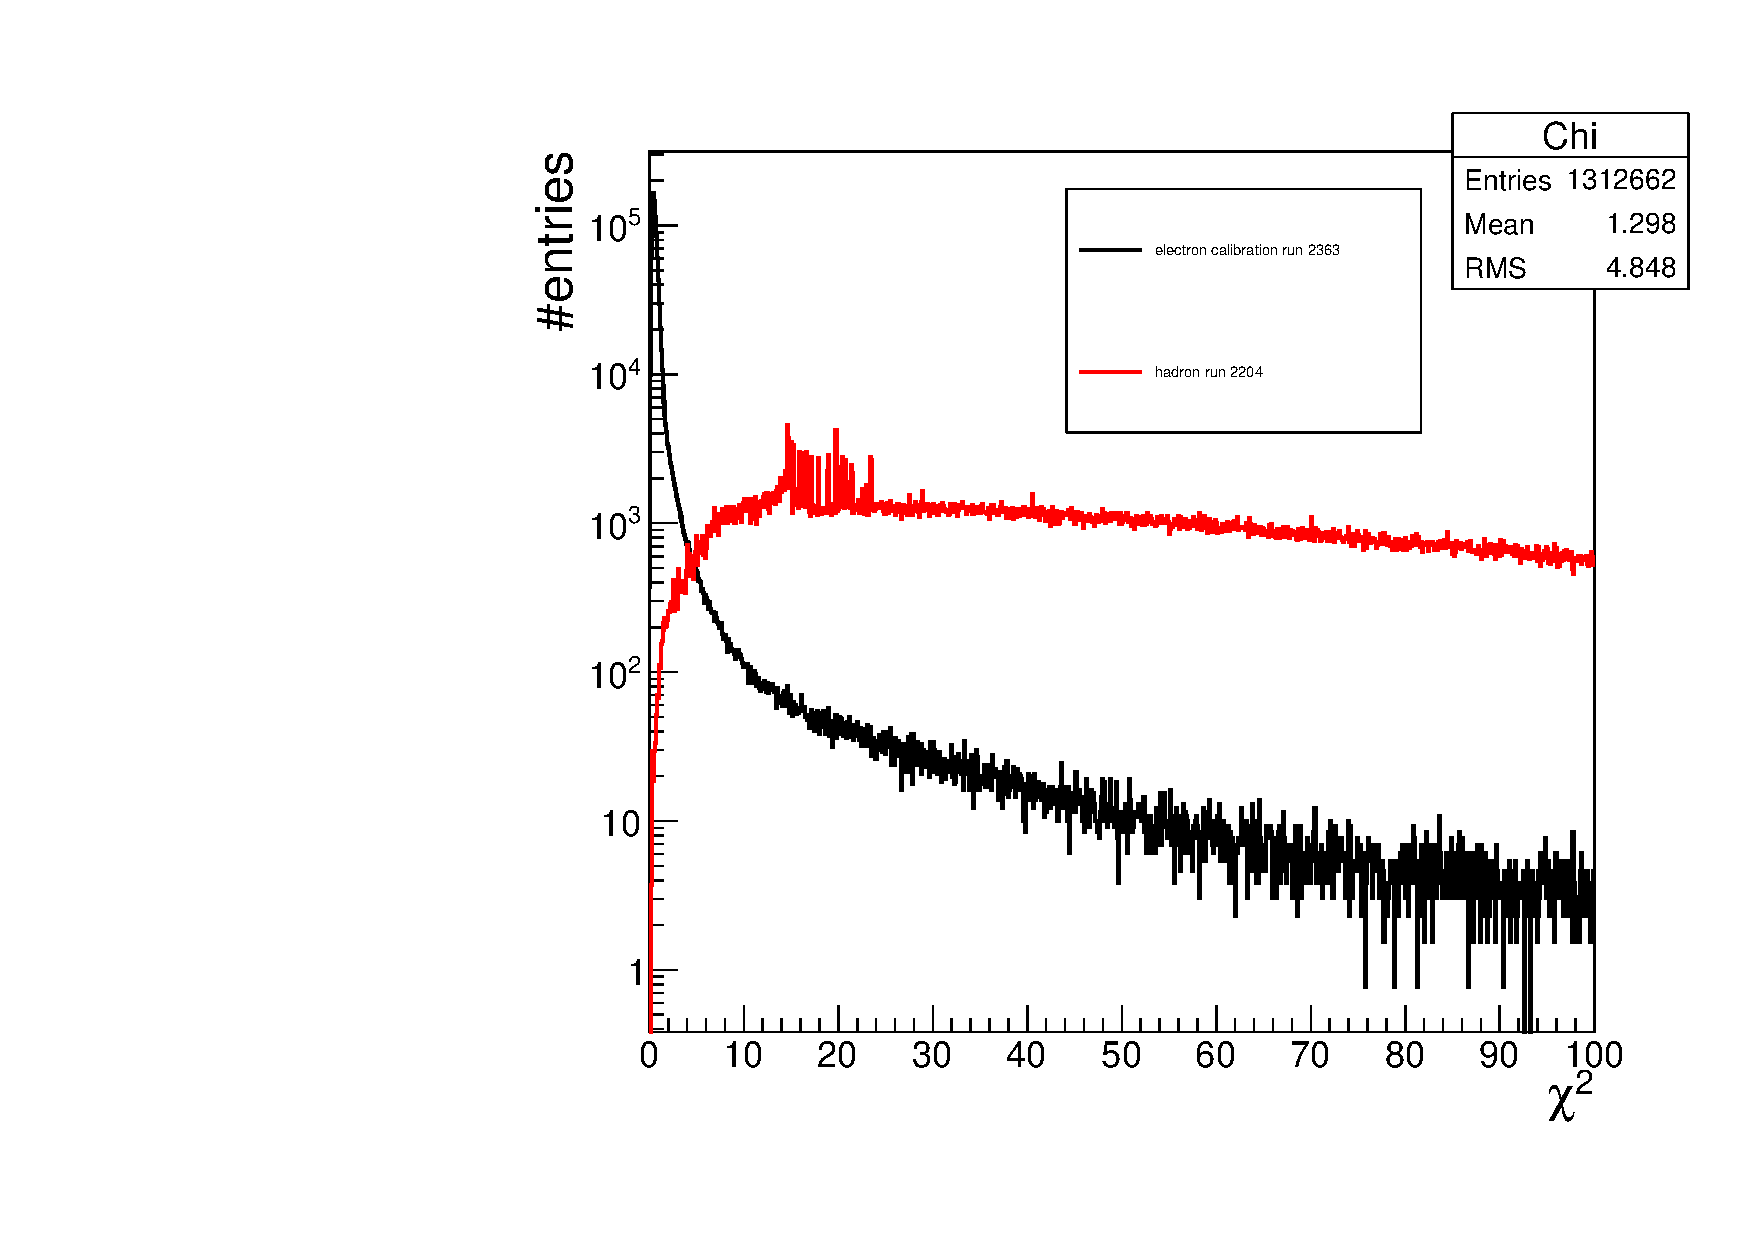
\includegraphics[width=0.95\textwidth,height=0.8\textwidth]{\pdirthree/chi_comp.pdf}
  \end{center}
  \caption[comparison between $\chi^2$ distribution, electron and hadron calibration run]{comparison between $\chi^2$ distribution generated from an electron calibration run (black) and hadron calibration run (red).}
  \label{fig:chi2}
\end{figure}

\begin{figure}[h!]
  \begin{center}
    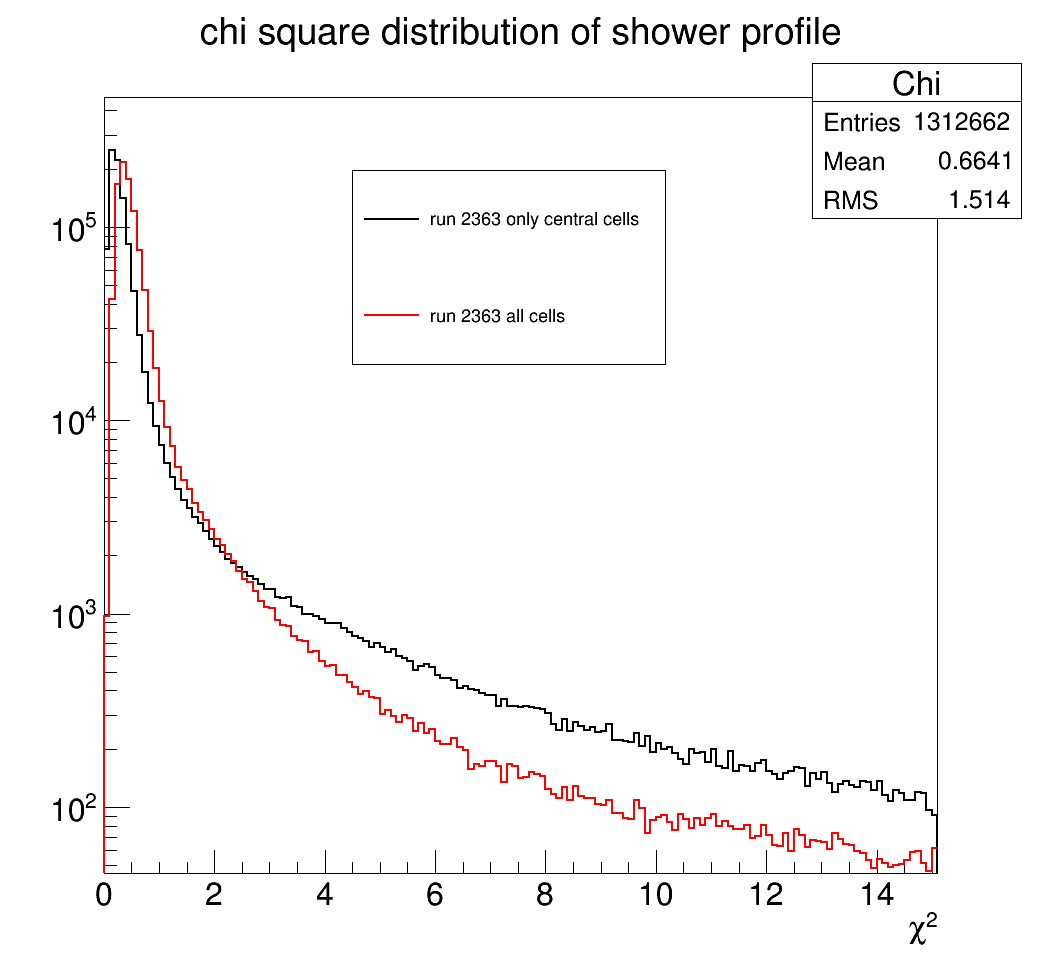
\includegraphics[width=0.95\textwidth,height=0.8\textwidth]{\pdirthree/plot_comp_cells.png}
  \end{center}
  \caption[comparison between $\chi^2$ distribution for different ECAL configurations]{comparison between $\chi^2$ distribution generated from an electron calibration run considering only central cells (black) and considering all 36 cells (red).}
  \label{fig:chi}
\end{figure}

\begin{figure}[h!]
  \begin{center}
    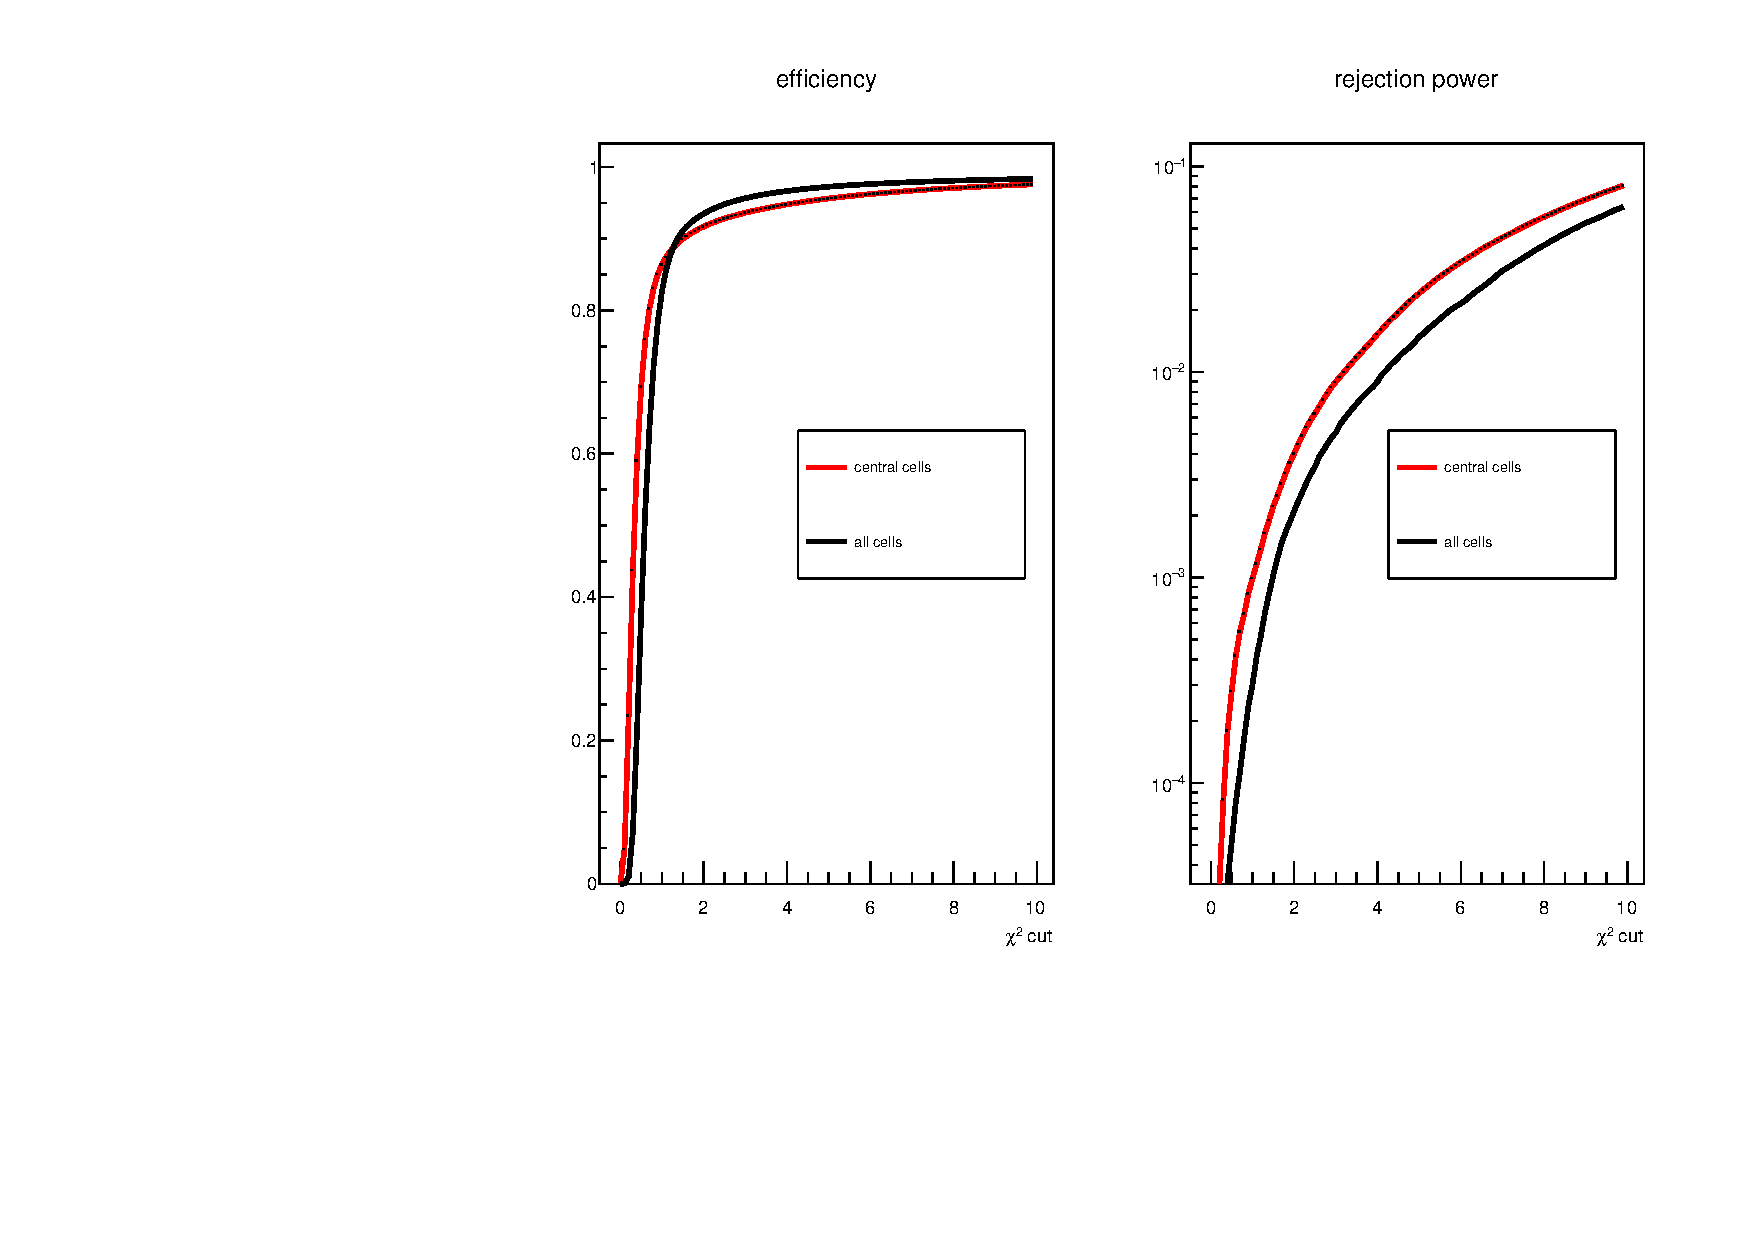
\includegraphics[width=0.95\textwidth,height=0.6\textwidth]{\pdirthree/eff.pdf}
  \end{center}
  \caption[fraction of events passing the $\chi^2$ cut]{fraction of events passing the cut $\chi^2 < \chi^2_{cut}$
    for the electron calibration run (left) and for the hadron calibration run (right).}
  \label{fig:eff}
\end{figure}

Different ECAL vs HCAL plots were produced to study the effect of a
$\chi^2$-cut for the run mentioned above. The one produced with
benchmark cut of $\chi^2 < 2$ are shown in
Fig.\ref{fig:ehcal_test}. The cut is shown to clean the plot in the
way expected from the hadronic activity in all selected runs. It can also
can be seen from the run recorded with physical trigger that events involving the dimuon
production $e^- \to \mu^+\mu^-$ survive the cut for energies larger
than 20 GeV.  This is expected since these events will still involve
an electromagnetic shower truncated in the moment the transition
happens. Since a possible signal from a Dark Photon would behave
similarly this suggest that the cut won't reject the signal provided
that the shower has enough energy. A similar study performed with the
MC reached the same conclusion, however for
very small energies the shower shape will slowly reach the energy
resolution in each cell and the efficiency of the cut will drop
substantially.  The efficiency for low energy improves if only central
cells are selected for the $\chi^2$ calculation since this will reduce
the fluctuation of the single cells not involved in the shower. This
effect is shown in Fig.\ref{fig:ehcal_comp} for a cut of 2 on $\chi^2$.
\\
\\
For low energy particles it is clear that all the shower will be
contained in the cell 3x3. Below this threshold shower analysis can no
longer resolve the type of shower of the event and instead the simple
requirement of the full energy of the event to be detected by the
central cell (3x3) should be used to avoid killing the
signal. Applying a $\chi^2$-cut to a dark photon simulation suggested that this limit is roughly 5 GeV.  The
left plot in Fig.\ref{fig:ehcal_comp} is compatible with this
estimate.

\begin{figure}[h!]
  \begin{center}
    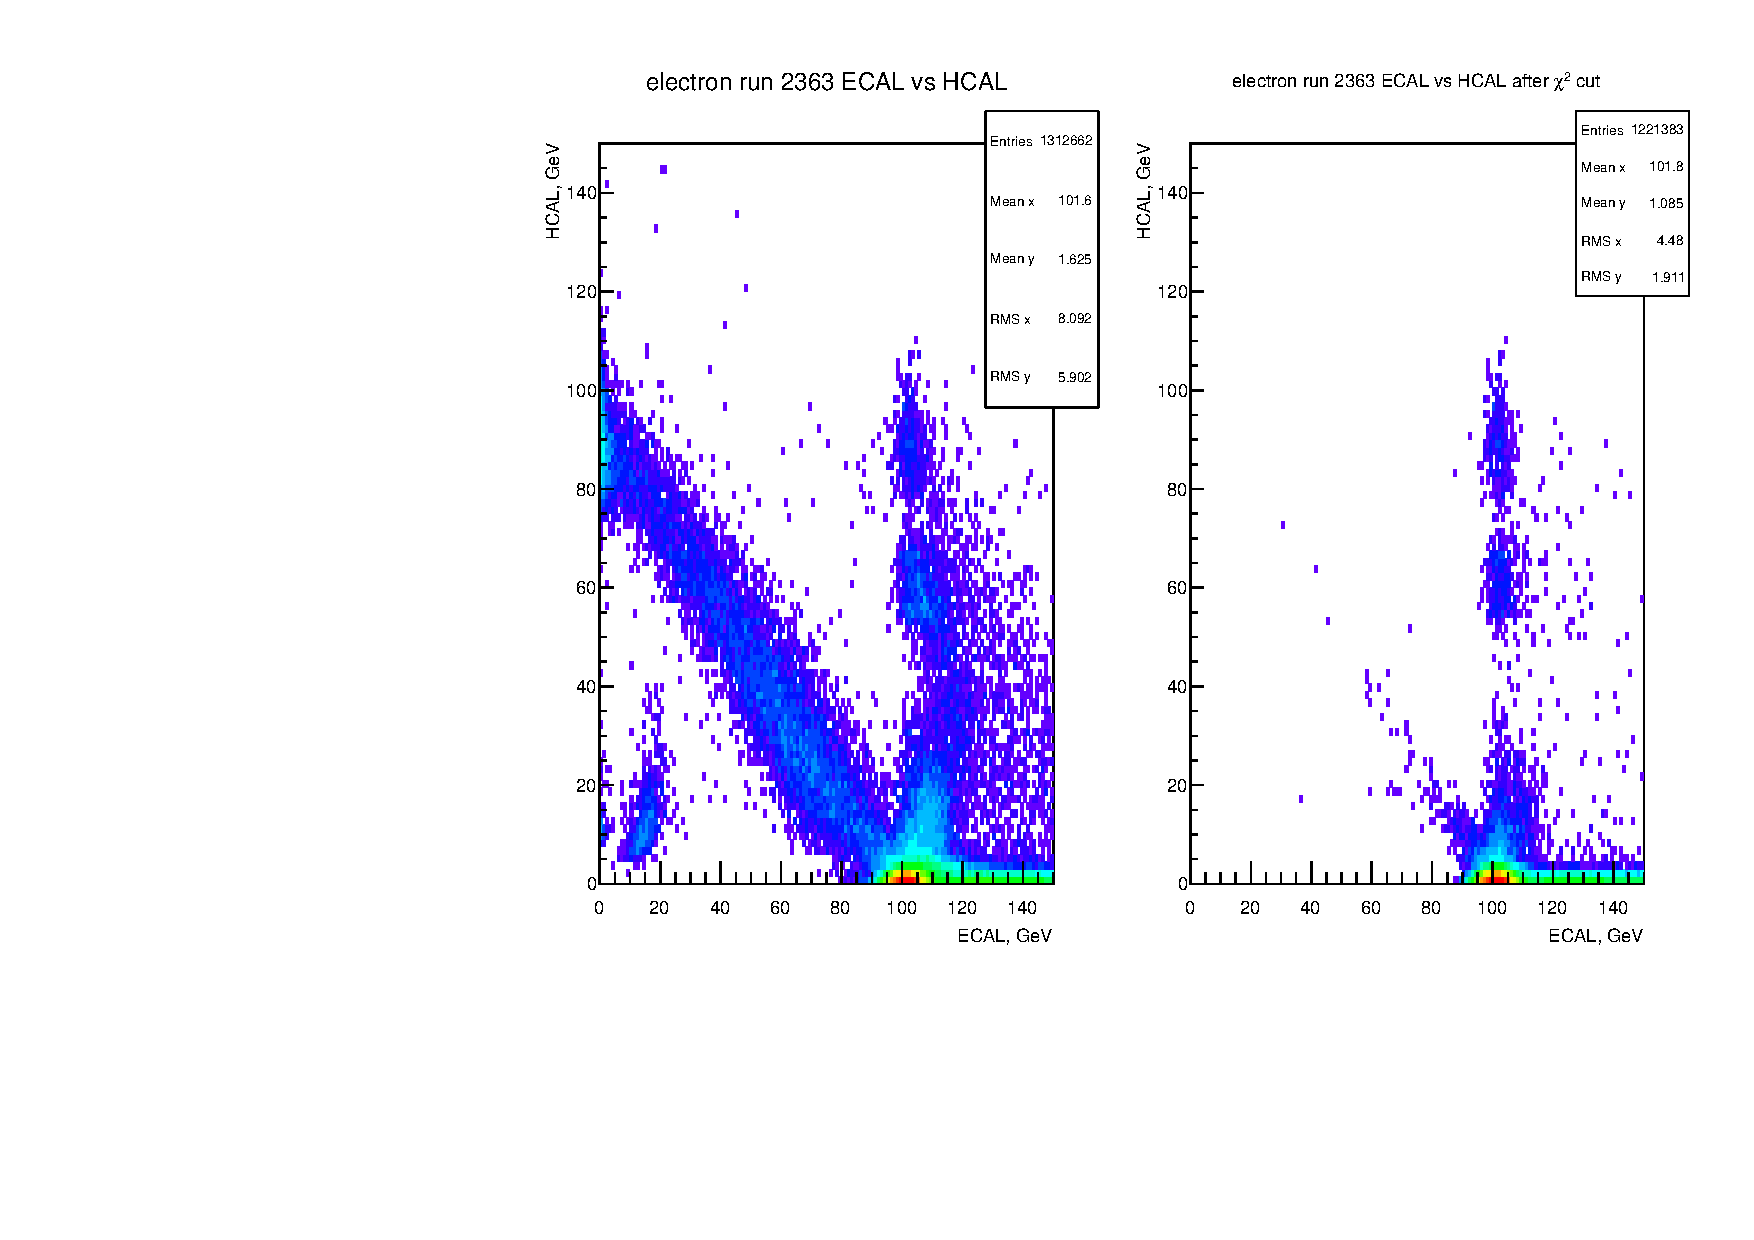
\includegraphics[width=0.95\textwidth,height=0.45\textwidth]{\pdirthree/ehcal_2336_chi.pdf}
    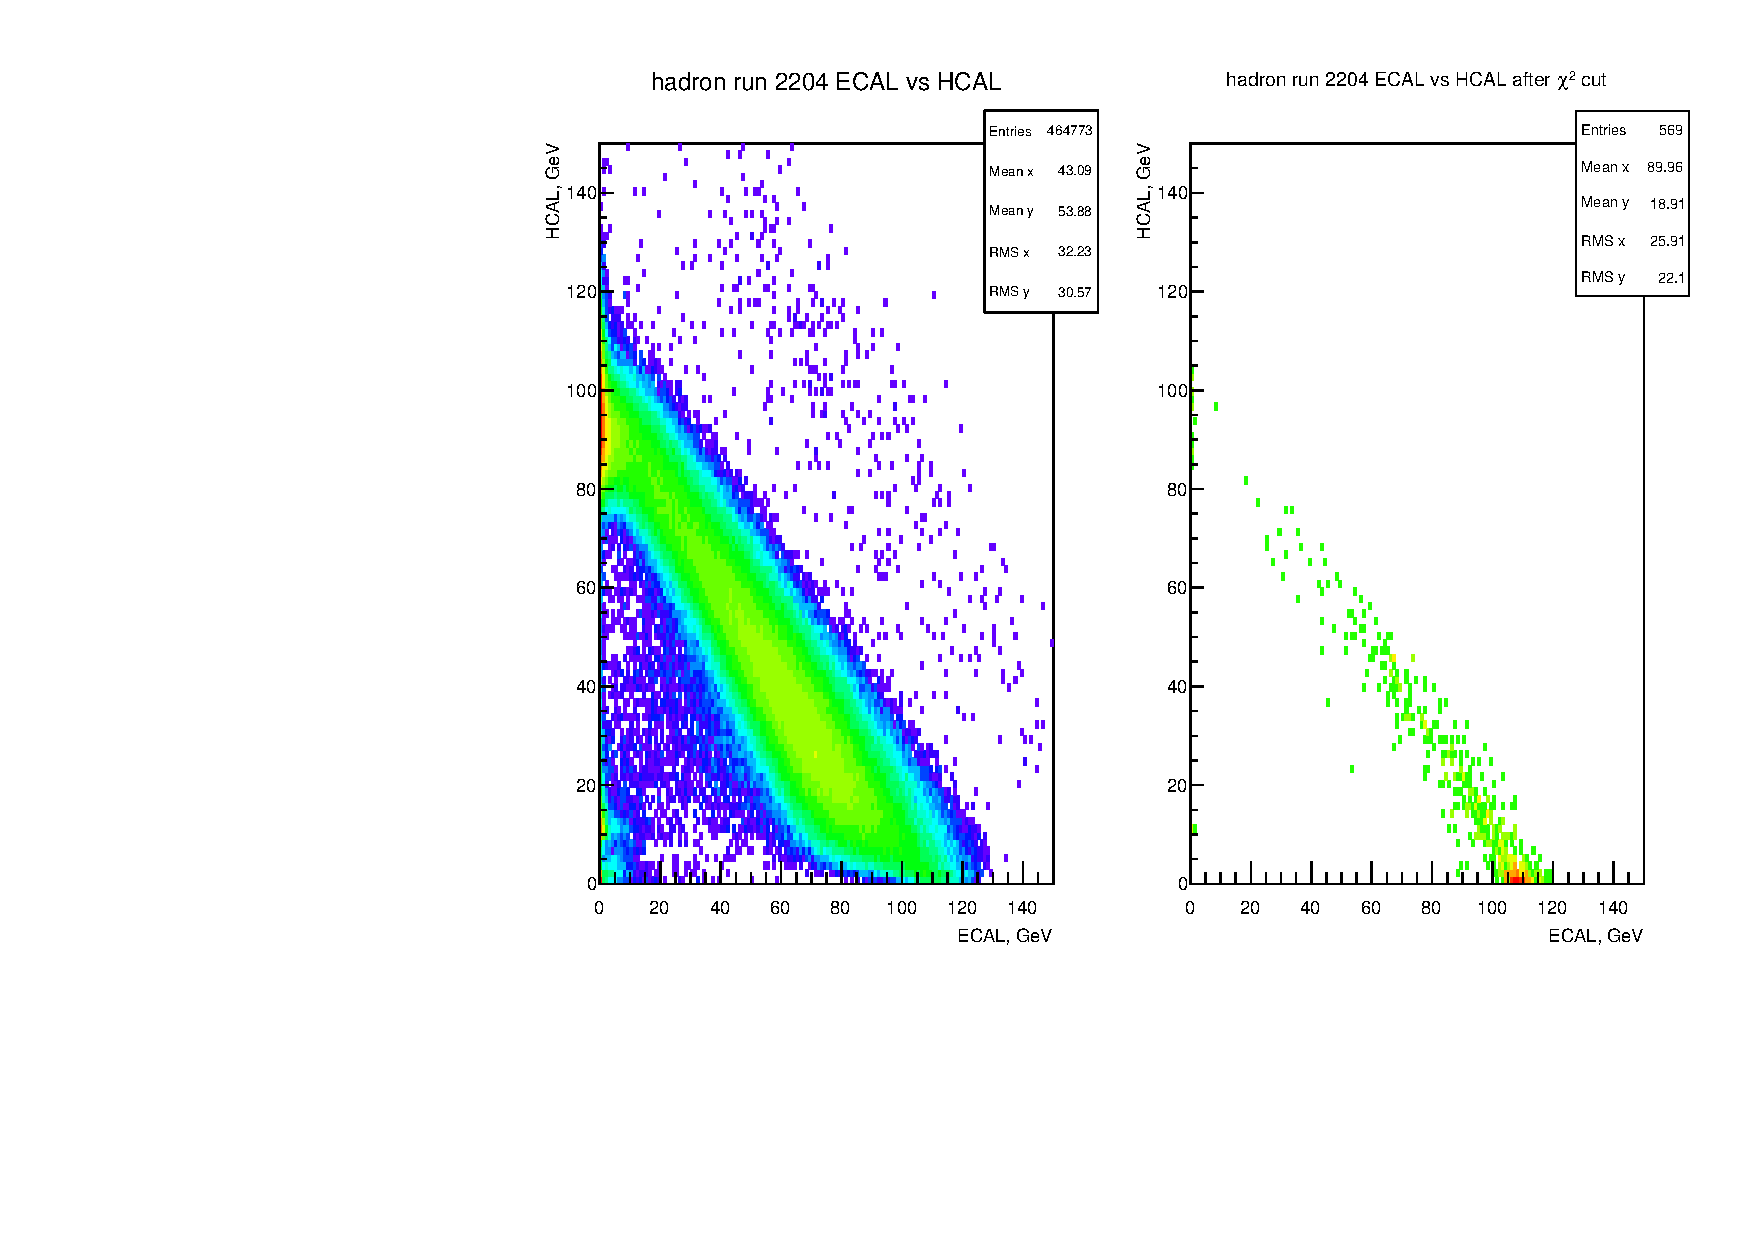
\includegraphics[width=0.95\textwidth,height=0.45\textwidth]{\pdirthree/ehcal_2204_chi.pdf}
    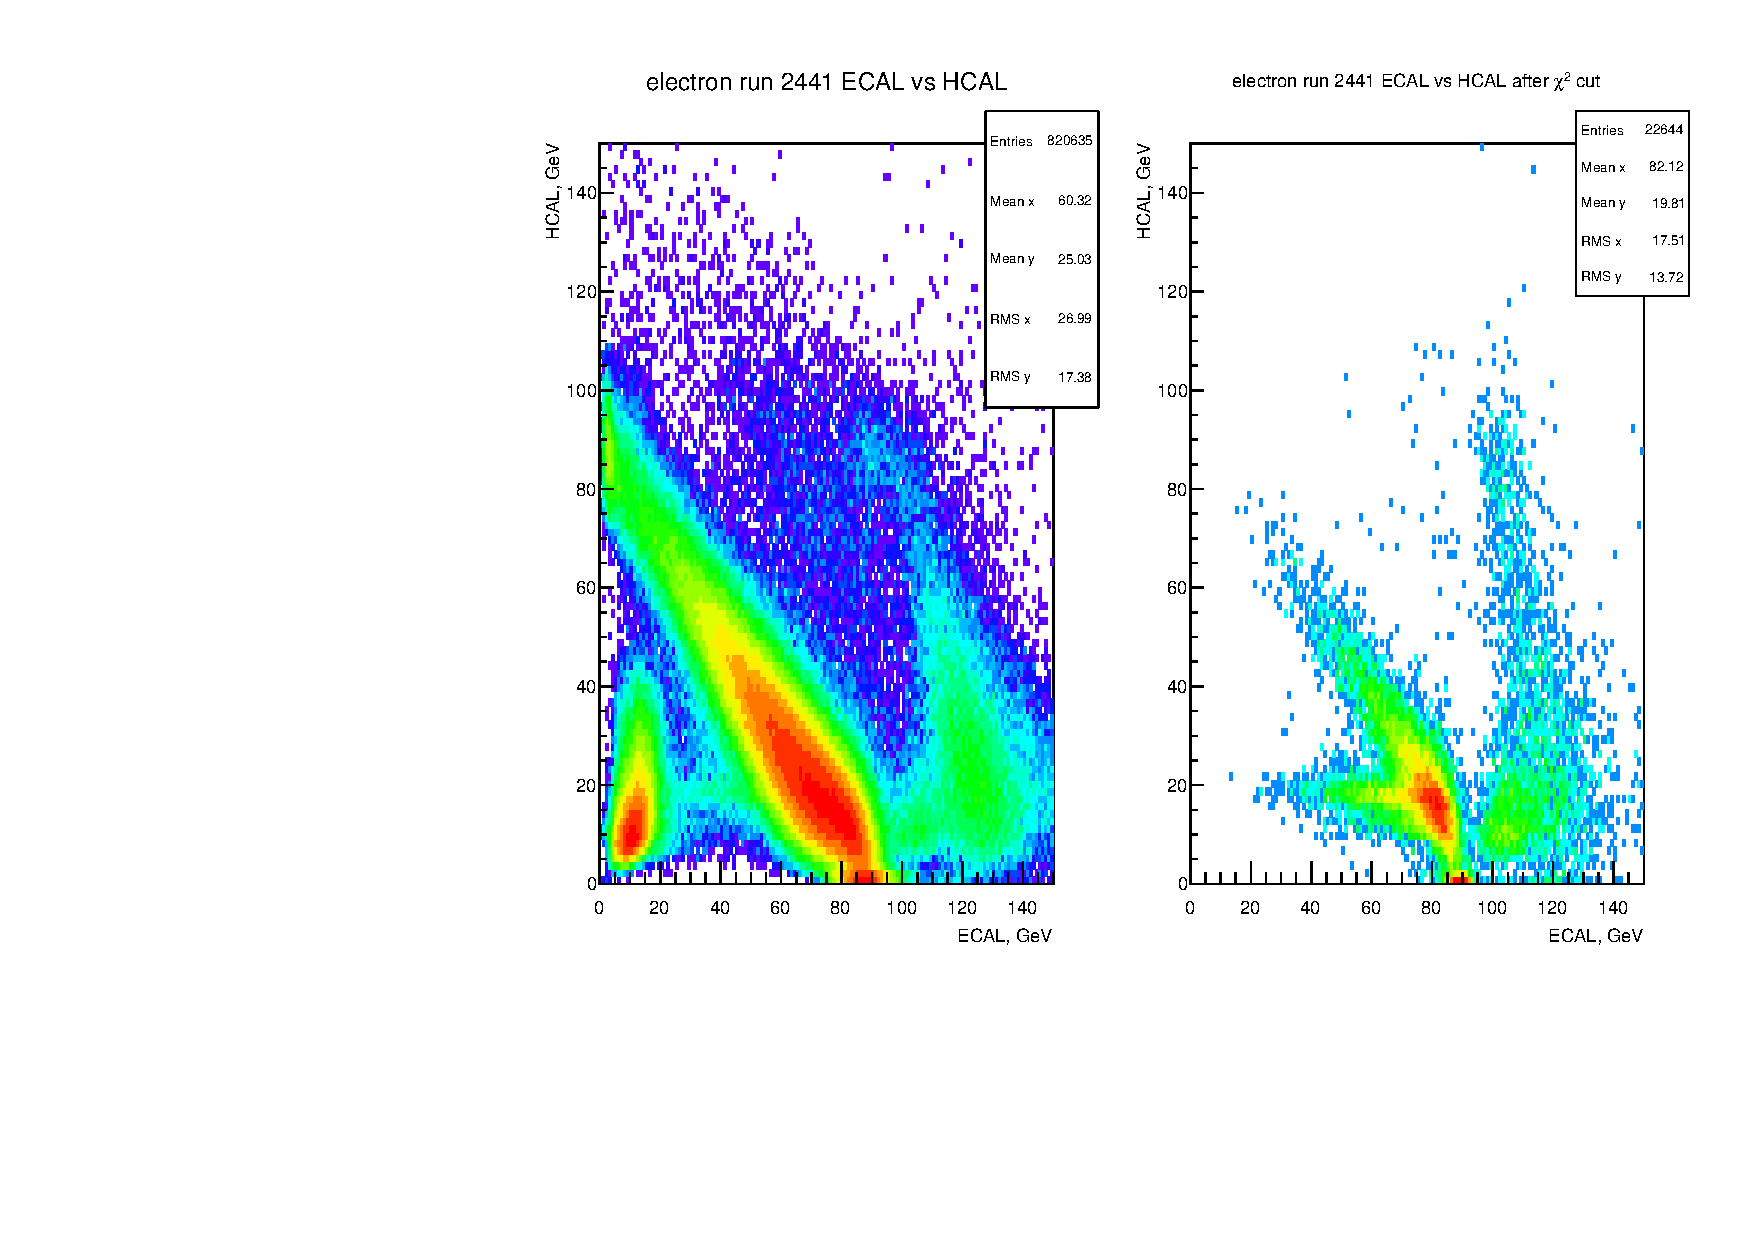
\includegraphics[width=0.95\textwidth,height=0.45\textwidth]{\pdirthree/ehcal_2441_chi.pdf}
  \end{center}
  \caption[ECAL vs HCAL energy deposit after a cut $\chi^2$]{ECAL vs HCAL energy deposit for the total sample (left
    column) and after a cut $\chi^2<2$ (right column) for the
    electron calibration run (top), the hadron calibration run (middle) and the run recorded with physical trigger(bottom).}
  \label{fig:ehcal_test}
\end{figure}
\clearpage

\begin{figure}[h!]
  \begin{center}
    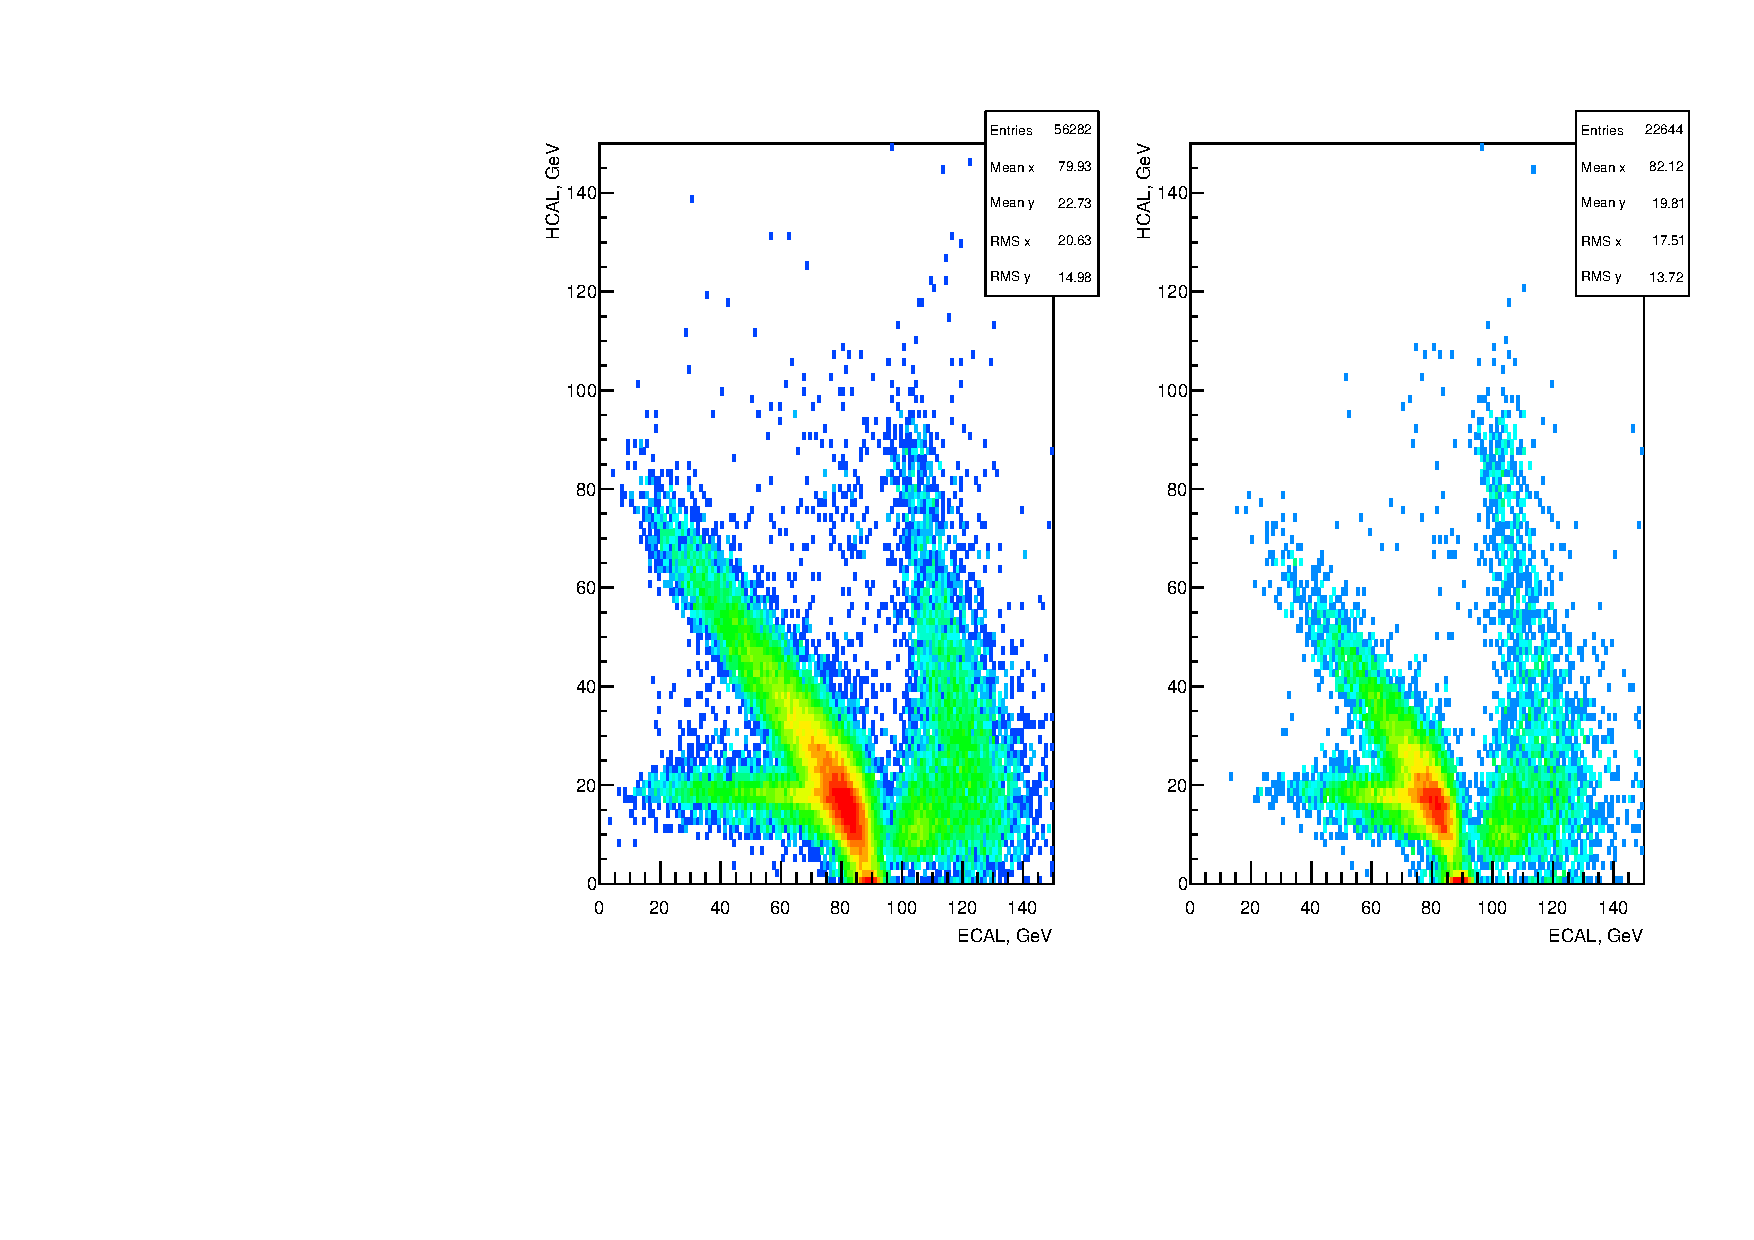
\includegraphics[width=0.95\textwidth,height=0.6\textwidth]{\pdirthree/ehcal_2441_comp.pdf}
  \end{center}
  \caption[ECAL vs HCAL energy deposit after a cut $\chi^2$ for different ECAL configurations]{ECAL vs HCAL after a cut $\chi^2<2$ is applied with the $\chi^2$ calculated with the 9 central cells (left) and for all cells (right).}
  \label{fig:ehcal_comp}
\end{figure}

\iffalse

\section{Comparison with MC}
\label{ch3:sec:mc}
The same profiles described in the section above can be produced using
a 100 GeV electron simulation of the NA64 setup\cite{na64-simulation} and be tested using simulation of $\pi^-$.

We tested qualitatively the effect of a $\chi^{2}$-cut over the
ECAL vs HCAL plots produced for both the MC simulation
and the test runs considered in the previous section. For the
MC-simulation we used the same benchmark cut of the previous section
$\chi^2_{cut}$=2 , while for the data a benchmark cut of
$\chi^2_{cut}$=40 was used to take into account the shift in the
distribution observed.

The bottom plot of Fig.\ref{fig:ehcal_elec} shows that the
contamination of hadron is removed when MC-database is used, so
the hadron shower still produces a significantly larger $\chi^{2}$
compared to the one of an electron shower. The efficiency
observed in the simulation is of ~0.98, slightly larger compared to the data. 
In both simulation and data we can observe that the characteristic
Di-muons events in the range [40,80] GeV in ECAL energy
deposition are accepted.
Fig.\ref{fig:ehcal_hadr} also shows the hadrons to be rejected in both
cases, with a rejection power of $\sim 5\times 10^{-3}$ measured in the
simulation. Also for both simulation and data we can observe that the
events surviving lie mostly in the diagonal $E_{ECAL}$+$E_{HCAL}$= 100
GeV (as could also be observed using a database built from calibration run like in Fig.\ref{fig:ehcal_comp}), while all the events where the shower has large angular spread are rejected.
\\
The main difference between the two plots concerns some events with very low energy deposited in the ECAL that are accepted in the data but not in the simulation. This would suggest that the ECAL cells are subject to some fluctuation that at low energy can sometime mimic the correct electromagnetic-shower signature. As stated in the previous section however for such low energy events the usage of the shower-profile algorithm should be avoided since all the shower will be completely contained in the cell 3x3.\\
% Finally the MC-database was applied to the physical run 2441 always
% with a benchmark cut $\chi^2_{cut}$=40.


\begin{figure}[h!]
  \begin{center}
    \includegraphics[width=0.95\textwidth,height=0.8\textwidth]{\pdirthree/ehcal_2363_chi_mc_2.pdf}
  \end{center}
  \caption{\textbf{Top}: ECAL vs HCAL before (left plot) and
    after (right plot) a cut
    $\chi^2<2$ in MC simulated 100 GeV electron events. \\
    \textbf{Bottom}: ECAL vs HCAL before (left plot) and after (right
    plot) a cut
    $\chi^2<40$ in the electron run 2363.\\
    The $\chi^2$ was computed using all ECAL cells with a shower
    profile database obtained from a 100 GeV $e^-$ MC-simulation. }
  \label{fig:ehcal_elec}
\end{figure}

\begin{figure}[h!]
  \begin{center}
    \includegraphics[width=0.95\textwidth,height=0.8\textwidth]{\pdirthree/ehcal_2204_chi_mc_2.pdf}
  \end{center}
  \caption{\textbf{Top}: ECAL vs HCAL before(left plot) and
    after(right plot) a cut
    $\chi^2<2$ in MC simulated 100 GeV $\pi^-$ events. \\
    \textbf{Bottom}: ECAL vs HCAL before (left plot) and after (right
    plot) a cut
    $\chi^2<40$ in the hadron run 2204.\\
    The $\chi^2$ was computed using all ECAL cells with a shower
    profile database obtained from a 100 GeV $e^-$ MC-simulation. }
  \label{fig:ehcal_hadr}
\end{figure}
\fi

\section{Invisible mode analysis}
\label{ch3:sec:analysis-invis}

The general method of analysis described in Sec.\ref{ch3:sec:analysis-approach} is now applied to the specific case of the invisible mode data. To apply the method a set of selection criteria is set to maximize the overall sensitivity of the setup using the MC-simulation described in Sec.\ref{ch3:sec:geant4}. The background is also detailed using the classification defined at the beginning of this chapter. We will show that the expected number of events in the signal region in absence of Dark Photon production is $\simeq 0.5$, making NA64 a background-free experiment.

\subsection{Selection criteria}
\label{ch3:sec:selection-criteria}

We define here the selection criteria used in the analysis to maximize our sensitivity. The cuts used are chosen based on their significance in the MC simulation, defined as:

\begin{equation}
  \label{eq:significance}
  S = \frac{s}{\sqrt{s + b}}
\end{equation}

In this context, the signal is not necessarily an event with $\DMM$ production, but the particle that the cut is supposed to select. In the case of SRD for example, the cut is required to select electrons and reject any other kind of particle. So $s$ will be the number of electrons selected by the cut and $b$ will be the number of non-electron ($\pi^-$, $\mu^-$ selected). Since only $e^{-}$ can trigger the reaction $\ea$, this requirement also maximizes the sensitivity of the experiment. The cuts are then optimized using the calibration run and control sample to take into account the effect caused by pileup and electronics as explained in Sec.\ref{ch3:sec:analysis-approach}.

%\subsection{Invisible mode}
%\label{ch3:sec:selection-criteria-invis}

The selection criteria needs to select 100 $\gev$ electrons and reject any events involving interactions before reaching the target. Events are accepted if they surpass the following criteria:

\begin{itemize}
\item The difference between the reconstructed momentum and the nominal beam energy of 100 $\gev$ is not larger than 5 $\gev$. Additionally, the entrance angle of the particle needs to be within 2 $\mrad$ from the mean angle recorded in the calibration run. The track also needs to be reconstructed with a $\chi^2<5$.
\item A deposit of at least 1.3 $\mev$ and not larger than 80 $\mev$ is required in each SRD crystal. Each signal is also required to be in a window of 5 $\nas$. To reject large backscattering from the ECAL, the maximum energy of 120 $\mev$ is allowed in total in the SRD. These cuts ensure the suppression of heavy charged particles in the beam.
\item The energy deposited in the ECAL is required to be in time with $S_0$ within 13 \nas. If more than 30 $\gev$ energy is recorded out of time, the event is rejected. Furthermore, the largest energy deposit in the ECAL needs to be in the ECAL central cell\footnote{The cell is labeled (3$\times$3), a sketch can be seen in Fig.\ref{fig:ecal_example}}. The periphery of the shower is also checked by taking the ratio between the energy deposited outside of the 3$\times$3 matrix that surrounds the central cell and the total energy deposited in the ECAL. Since most of the energy of an em-shower will be deposited inside the Moliere radius, the value outside of it should be below 5\% of the total energy deposited. Finally, the compatibility with an em-shower is checked using the method described in Sec.\ref{ch3:sec:bkg-ecal-profile} with a cut $\chi^2 < 8$.
\item All events with signal above noise in the VETO are rejected to avoid punch-through from the main target. The precise value of the cut is defined as 0.9$\times \emip$.
\item Events where the energy deposited in one of the cells in the periphery of the HCAL is larger than the one deposited in the center are rejected.
\item Events with multiple hits in the straw chamber are removed from the analysis. This cut is used to remove the contamination due to electron-hadron production upstream of the ECAL.
\end{itemize}

Finally, the signal region is defined by events with significant missing energy in the ECAL and no activity in the HCAL. This means $E_{ECAL} < 50$ $\gev$ and $E_{HCAL} < 1$ $\gev$, previously illustrated in Fig.\ref{fig:two-signature}.

The efficiency of the cuts listed above was studied using the MC simulation and the electron calibration runs.
%A small summary of the uncertainty is provided in Table \ref{tab:inv-cut-eff}.
The effect of these cuts can be appreciated in the $\ehcalplane$ plane where the signal region is defined. They are shown in Fig.\ref{fig:inv-cut-ehcal}, most notably the amount of hadrons is seen to greatly reduced after the SRD cut is applied, and consequentially the dimuon region becomes more visible. The VETO cut then removes most of the punchthrough particles, including dimuons. Finally, when the tracking selection criteria are applied, a large portion of the low energy deposit event and strong scattering upstream disappear\footnote{This is mostly visible in the requirement of "GoodTrack", visible between plot 5 and 6}.


\begin{figure}[bth!]
  \centering
   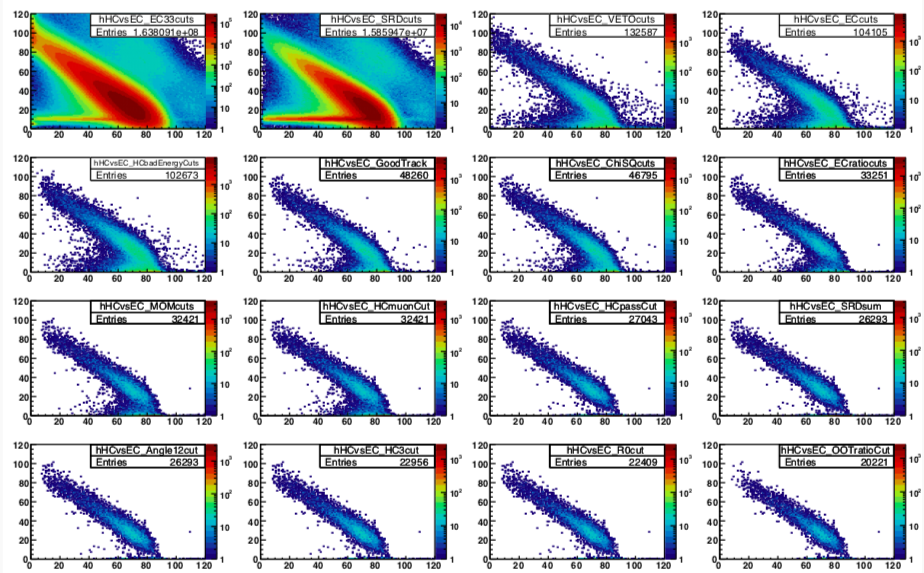
\includegraphics[width=\textwidth]{\pdirthree/ec-hc-plots-veto-nobad-runs.png}
  %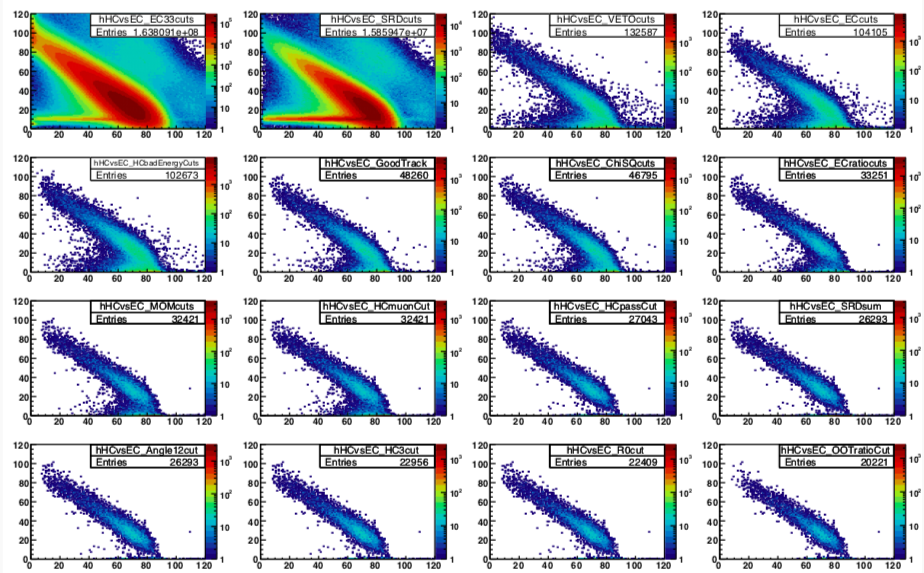
\includegraphics[width=\textwidth]{\pdirthree/ec-hc-plots-veto-nobad-runs.pdf}
  \caption[effect of the cuts in invisible mode]{Effect of selection criteria in the $\ehcalplane$ on the sample of data collected in 2018 invisible mode \cite{invis-cut-plot,NA64:2019imj}.}
  \label{fig:inv-cut-ehcal}
\end{figure}

\subsection{Background}
\label{ch3:sec:bkg:inv}

In this section, we will try to go more in detail of what constitutes background in invisible mode setup, following the classification defined in Sec.\ref{ch3:sec:analysis-approach}. A complete summary of the expected background, including uncertainty for each single source, is provided in Table \ref{tab:inv-bkg}.
\subsubsection{Hadronic background}
\label{ch3:sec:bkg:inv:hadr}


In the case of invisible mode, the \textbf{Hadronic background} can arise simply from a $\pi^-$ that after leaving minimal energy in the ECAL, travels through the HCAL undetected. The probability of this happening with a total interaction length of 21 $\lambda_{int}$ is $p\lesssim 10^{-9}$. This number does not account for the high-efficiency VETO after the ECAL, SRD rejection, and the fact that the HCAL can detect a MIP interaction even without an inelastic interaction happening. Each of these factors pushes the background well below $<10^{-13}$ as pointed out in the NA64 first proposal \cite{Andreas:2013lya}.

A more significant background is caused by the inelastic scattering inside the ECAL in a process:

\begin{equation}
  \label{eq:pion-nucleus-scattering}
  h + Z \longrightarrow h + Z + (hadrons)
\end{equation}

Here, part of the energy can evaporate as a consequence of some particles emitted at a large angle and thus escaping the setup in the direction transverse to the beam. This background is suppressed by shower profile analysis, energy deposited in the pre-shower, and the VETO cut. The phase space of this process is however complicated, and a lot of possible phenomenologies can arise from it. For example, large energy deposited in the pre-shower can be a simple consequence of some $\pi^0$ backscattering after the hadronization, while the shower profile can mimic the one of an electron if a large fraction of energy in the inelastic scattering is carried away by $\pi^0$. Also, if particles are emitted in the form of neutrons or other neutrals as $\ks$, the VETO would be ineffective to reject them.

To have an estimate, we can take the process \ref{eq:pion-nucleus-scattering} and assume $\geq$2 neutrals particles are produced in the hadronization. This gives us a probability equal to \cite{gkkk1}:

\begin{equation}
  \label{eq:transverse-leak-estimate}
  P \simeq P_n \cdot P_{la} \cdot P_{leak}
\end{equation}

Where we define $P_n$ the probability of such interaction to occur, $P_{la}$ the probability to produce particles at large scattering angle, and $P_{leak}$ the probability to escape HCAL without interactions. Here we stress again that this formula hides a large number of topologies that such an event could have, but is instructive to get an intuition for these processes. Since the ECAL has $\lambda_{int} \simeq 0.5$, the probability of interaction for an hadron is fairly high (roughly 50\% of the time such interaction will happen). We need at least 50 $\gev$ of energy leaking to produce a signal event. If we assume two neutrals to be produced at $\Theta_{n} \simeq 30$\si{\degree} this would mean crossing at least 4$\lambda_{int}$ each, for a $P_{leak} \lesssim 3 \cdot 10^{-4}$. We can take the measured values of NOMAD to estimate the value of the cross-section in this range \cite{AUTIERO1998285,GNINENKO1998583}. The probability of separating a cluster with energy $>$0.1E$_{\pi}$ at an angle $\Theta_{n} \gtrsim 30$\si{\degree} was measured to be P$_{la} \simeq 10^{-5}$ and it drops very quickly with the beam energy: a factor 20 difference was found between 15 $\gev$ and 6 $\gev$ $\pi^-$. Even if we take this conservative value as $P_{la}$, see that the probability of the energy to escape is already $P\simeq 10^{-9}$, which multiplied to the hadron contamination and SRD suppression leads to an estimate of $P<10^{-14}$ for this background.

Another possible background is the decay of hadron inside the setup in neutrinos, which would cause some energy to disappear from the setup. The high energy of the primary suppress this background, since at 100 GeV the chance for a $\pi^-/K^-$ to decay is $P^{decay}_{\pi} \simeq  10^{-2}$. Multiple possible decays are accompanied by a neutrino emission, the most likely one being $\pi^- \rightarrow \mu^- +\nu_{\mu}$. The emission of the muon makes such decay very easy to spot, since it will leave an energy deposit both in the VETO and the HCAL, for a total probability similar to the one of a punch-through $\pi^-$ ($P < 10^{-14}$). One could argue that the $\mu^-$ could decay: $\mu^- \rightarrow e^- + \nu_{\mu}+ \bar{\nu_{e}}$, producing an electromagnetic shower with missing energy. The long decay time of the $\mu^-$ adds however an additional suppression factor of $P\simeq 10^{-5}$, which together with the upstream selection criteria put the background conservatively at $P \lesssim 10^{-13}$.

Another background comes from the decay $K^- \rightarrow \pi^0 + e^- + \bar{\nu_e}$, commonly called $K^-_{3e}$, with a branching ratio of $\Gamma_i/\Gamma_{tot} \approx$0.05 \cite{particle-strange-mesons}. The total probability of background for an incoming $K^-$ is around $P\simeq 10^{-3}$ accounting for both probabilities of decay and branching ratio. A MC-simulation of $K^-$ confirms this simple estimate as shown in Fig.\ref{fig:kaonbkg-sim}, where the fraction of the events in the signal region corresponds to the probability calculated. Multiplying this probability for the SRD selection criteria and the suppression from the beam returns a probability of $P_{K_{3e}} < 10^{-12}$. %\footnote{Here a suppression from the beam of 10$^{-3}$ is used, since the $K^-$ is a smaller fraction than the contamination \cite{h4-beamline}}.
There are however additional factors of rejection for this background that can be investigated using MC-simulations. A more precise account of SRD in this scenario and the effects of the tracking and shower profile push this background to $P_{K_{3e}} \lesssim 10^{-13}$.


\begin{figure}[bth!]
  \centering
  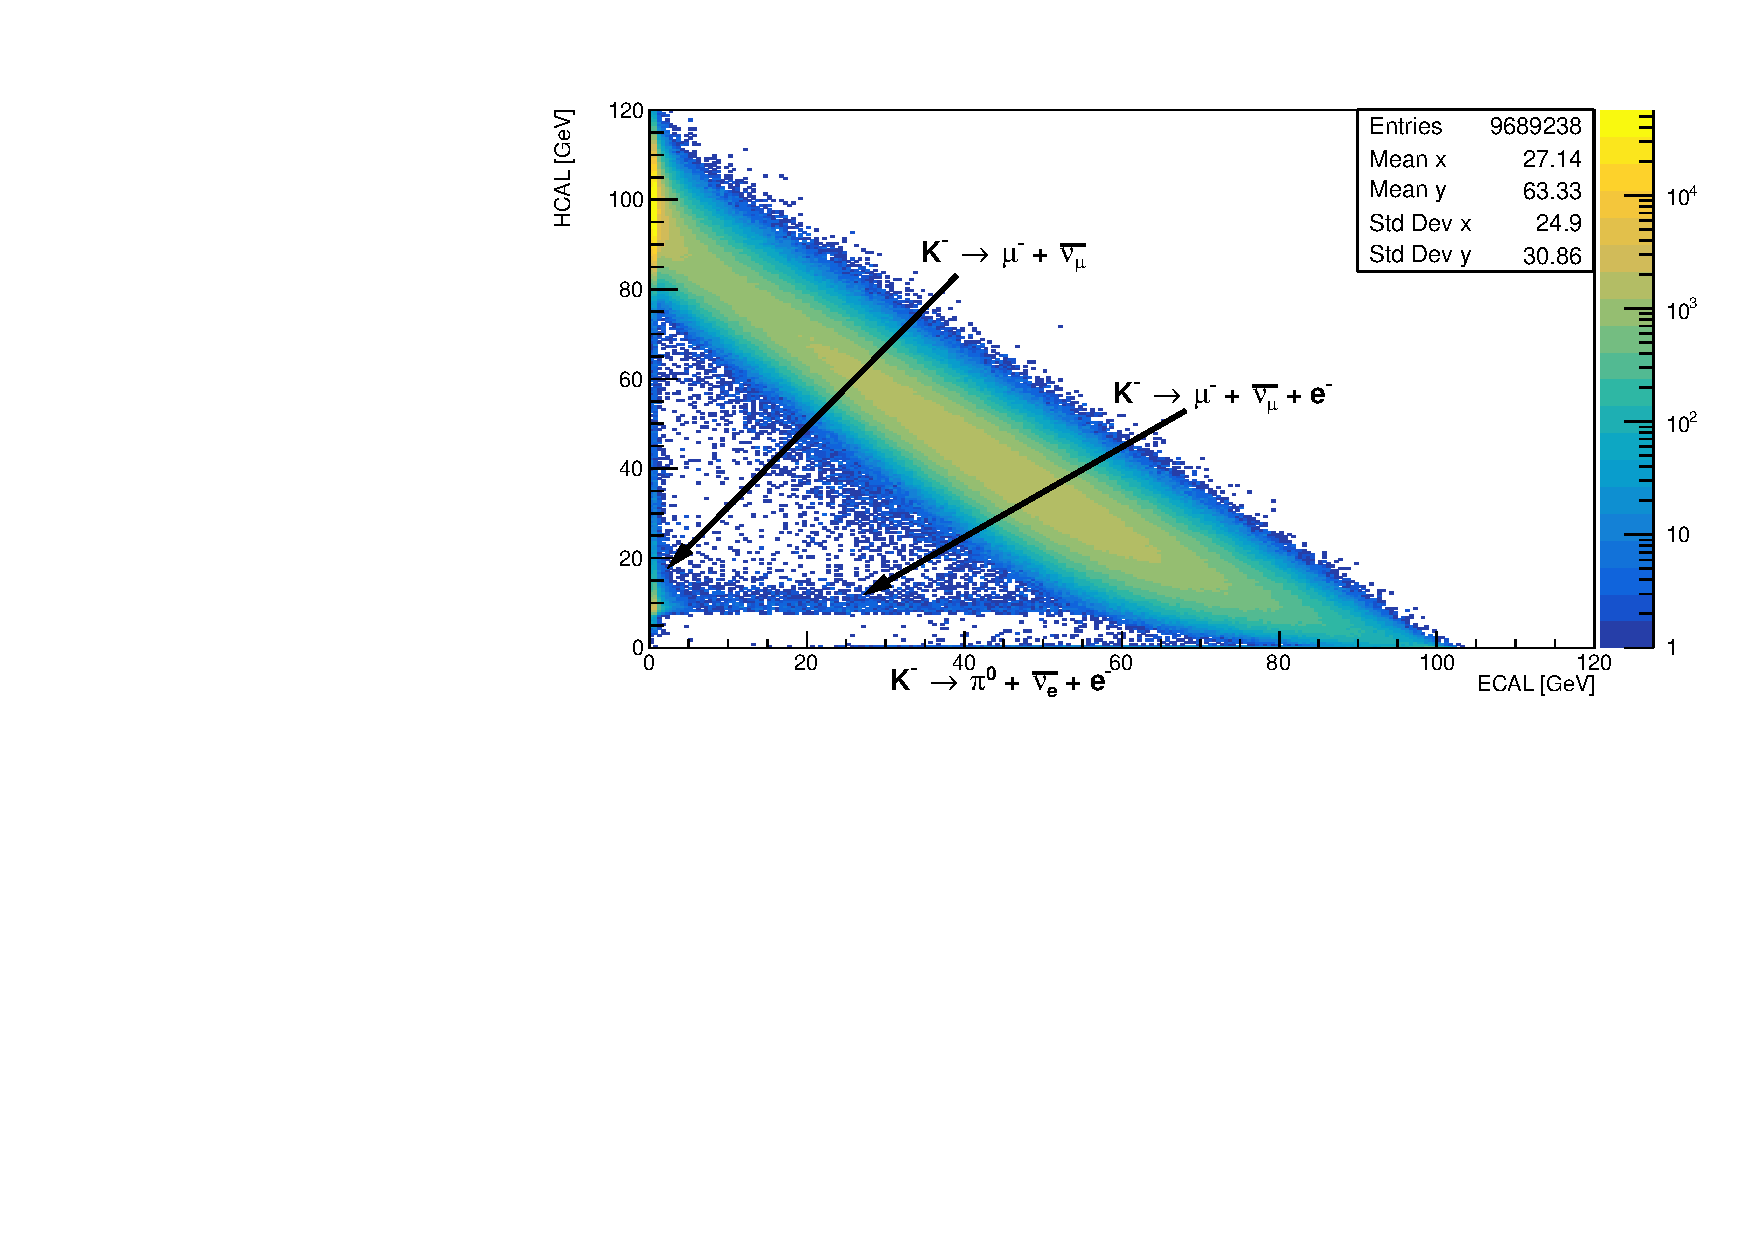
\includegraphics[width=\textwidth]{\pdirthree/kaonbkg.pdf}
  \caption[$K^-$ simulation ]{Energy deposited in the $\ehcalplane$ plane after simulating $10^7$ $K^-$ as primary particle in the NA64 setup.}
  \label{fig:kaonbkg-sim}
\end{figure}

\subsubsection{Muonic background}
\label{ch3:sec:bkg:inv:muon}

This type of background is also largely suppressed by both beam composition and SRD selection criteria, to a level of
%\footnote{Here the suppression from the beam composition is larger ($10^{-3}$) \cite{h4-beamline} and SRD selection criteria are more stringent ($10^{-4}$) due to the absence of back-scattering.}
$\lesssim 10^{-7}$. As in the case of $\pi^-$, we can convince ourselves that a complete punch-through of the setup without being detected is negligible. Indeed the muon needs to travel through both the VETO and 3 HCAL modules without leaving any detectable energy deposit. Using $p^{VETO} \simeq 10^{-3}$ for leaving undetectable energy in the VETO and $p^{HCAL} \simeq 10^{-4}$ to deposit less energy than the threshold in all modules, we see that the background is conservatively $< 10^{-14}$. In the case of muons, nuclear interaction is less likely. Thus, there is no chance for a large amount of energy to escape transversely. What remains is the decay $\mu^- \rightarrow e\nu\nu$, with neutrinos in the final state. The decay time of $\mu^-$ adds a suppression of $\lesssim 10^{-5}$. Similar to the previous case, proper accounting of SRD, tracking, and shower profile accounts for an additional $p\sim 0.1$ factor. The final level of this background is of $P_{\mu} \lesssim 10^{-13}$.

\subsubsection{Electronic background}
\label{ch3:sec:bkg:inv:elec}

The last type of background is originating from electron primary. Since the beam is primarily made of electrons, and SRD are tuned to select them, no upstream suppression factor can be achieved. Simple punch-through of an electron through the whole setup is not possible, since the path is blocked by 3 HCAL modules. Other similar events, with energy losses due to non-uniformity and cracks in the ECAL/HCAL were as well studied and found unrealistic \cite{Andreas:2013lya}. Low energy electrons is also potentially background: if a primary electron with $E_0 < E_{th}$ arrives at the ECAL it will leave an energy deposit compatible with the signal. Such a background was also found extremely unlikely. The amount of electron $N(E_e<E_{th})$ in the beam with energy lower than the energy threshold for the signal amounts conservatively to $<10^{-2}$. Such particles are normally deflected by the two MBPL magnets outside the acceptance of the ECAL\footnote{For $E_0$=50 $\gev$ the difference in deviation is about 0.4 \si{\meter}}. Particles with large entrance angle in the magnet can in principle enter in the acceptance of the magnet, but the tracking system makes sure that their energy is reconstructed with a resolution of $\delta p/p \approx 1\%$ \cite{Banerjee:2017mdu}. A dedicated simulation of $10^{10}$ EOT was performed by simulating electrons with energy compatible with the signal region. No event was found in the signal region after requiring a reconstructed momentum within 3$\sigma$. This allows us to put this background conservatively at a level of $\lesssim 10^{-13}$.

An important source of background to be considered is the dimuon production inside the target. As mentioned, these events are very useful to check for systematics and validated the MC. However, fluctuation in the energy deposited in the HCAL might leak in the signal region. The background was estimated by exponential extrapolation of the control sample inside the signal region ($E_{HCAL} < 1 \gev$) considering the sideband I depicted in Fig.\ref{fig:ehcal-bkg-bands}. This estimate was performed using the control sample without applying the VETO cut, that is then taken into account separately as a factor $\sim 10^{-6}$ (probability of two MIP to leave no energy).

\begin{figure}[bth!]
  \centering
  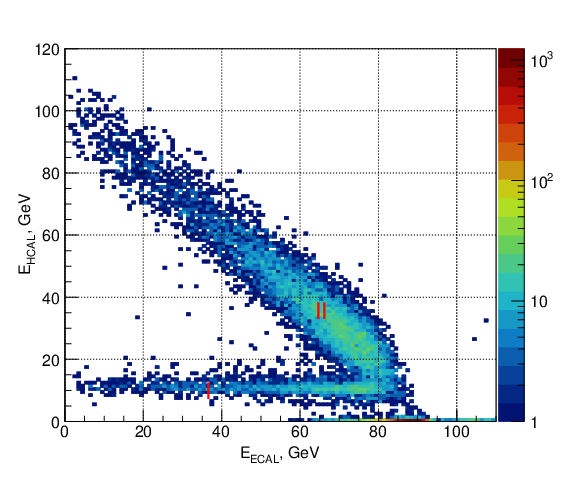
\includegraphics[width=0.45\textwidth]{\pdirthree/EHCAL_lastpub_left.png}
  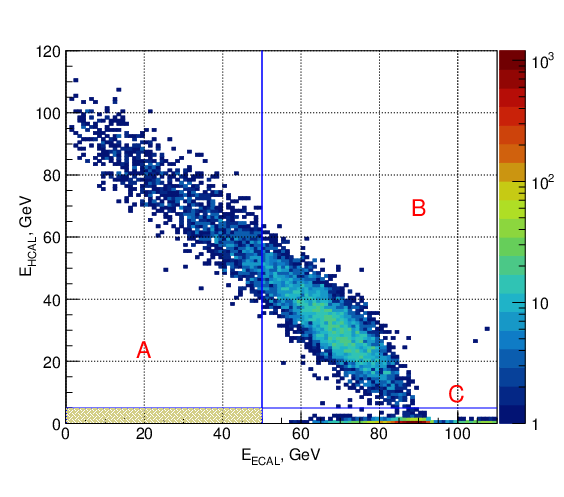
\includegraphics[width=0.45\textwidth]{\pdirthree/EHCAL_lastpub_right.png}
  \caption[ECAL vs HCAL events band]{Distribution of events in the $\ehcalplane$ plane for the control sample of the data. The right panel shows the sample with all the selection criteria. The left panel shows the same sample without the VETO cut. The shaded area is the signal box. The size of the signal box is increased by a factor 5 in the Y-axis direction for illustration purposes. The region labeled I contains events caused by dimuon production, while region II contains mostly event leaking from the ECAL into the HCAL. The sidebands A and C are used to estimate the background inside the signal region \cite{NA64:2019imj}.}
  \label{fig:ehcal-bkg-bands}
\end{figure}

Finally, the leading background in the invisible mode setup is the electro-nuclear and photo-nuclear production of neutral hadrons at a large angle. This case is similar to the one discussed for hadrons, but no additional suppression due to beam-composition and SRD selection criteria is present. In first approximation, the rarity of such interaction balances the absence of suppression factors, and accounts for $P_n \simeq 10^{-6}$ (see Eq.\ref{eq:transverse-leak-estimate}).
The largest source of background, however, comes from electro-nuclear production happening upstream of the target. As Fig.\ref{fig:eh-prod-sketch} shows, if this interaction happens in a detector with a large distance from the ECAL, the displacement of the particle can be large enough to exit the setup transversely. 


\begin{figure}[bth!]
  \centering
  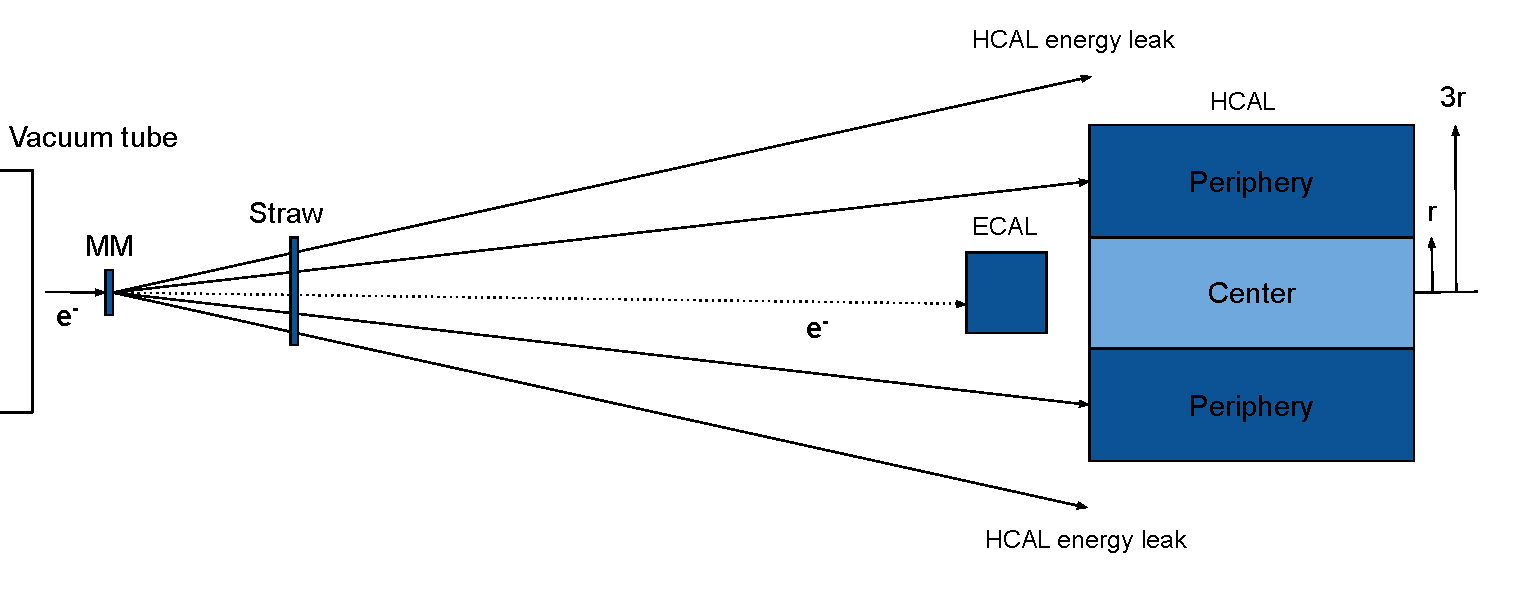
\includegraphics[scale=0.4]{\pdirthree/hcal-leak.pdf}
  \caption[upstream electro-hadron production upstream]{Sketch of electro-nuclear interaction happening upstream the ECAL leading to a possible background \cite{pdegen-thesis}.}
  \label{fig:eh-prod-sketch}
\end{figure}

This background can be estimated by looking at the periphery region of the HCAL. Since the angular distribution is sharply suppressed for large angle \cite{AUTIERO1998285,GNINENKO1998583}, these particles typically leave an energy signature in the periphery of the first HCAL when they miss the ECAL. For this purpose, we define the variable $R$ as the ratio between energy deposited in all cell excluded the central one, and the total energy deposited in the modules:

\begin{equation}
  \label{eq:R-factor}
  R = \frac{E^{all}_{HCAL} - E^{center}_{HCAL}}{ECAL^{all}_{HCAL}}
\end{equation}

In a normal event with particles leaking the ECAL, we typically observe $R<0.5$, as the HCAL module center is aligned with the beam direction, thus the dominating energy deposit will be in the central cell. If an electro-nuclear production happens upstream however, some distortion of this variable will be visible. In the most extreme scenario when the particle is missing the ECAL completely, the $R$ value will be equal 1, since the central cell of the HCAL will be shielded by the ECAL while the periphery will be directly hit. We can observe such behavior in Fig.\ref{fig:r-value-csample}: most of the event considered have an $R$ peaked at 0.35. Events, where the primary electron loses a large portion of its energy due to bremsstrahlung, are shown in region III and are responsible for events with large R. In this topology of events, the electron completely misses the ECAL after losing energy due to bremsstrahlung and being deflected by the magnetic field. The high-energy photon emitted propagates without being deflected and hits the HCAL in the periphery. Such events are also easily identifiable by looking at the HCAL placed in from the original beam direction. In the event of region III, this detector measure energy deposit $E>60$ $\gev$.

\begin{figure}[bth!]
  \centering
  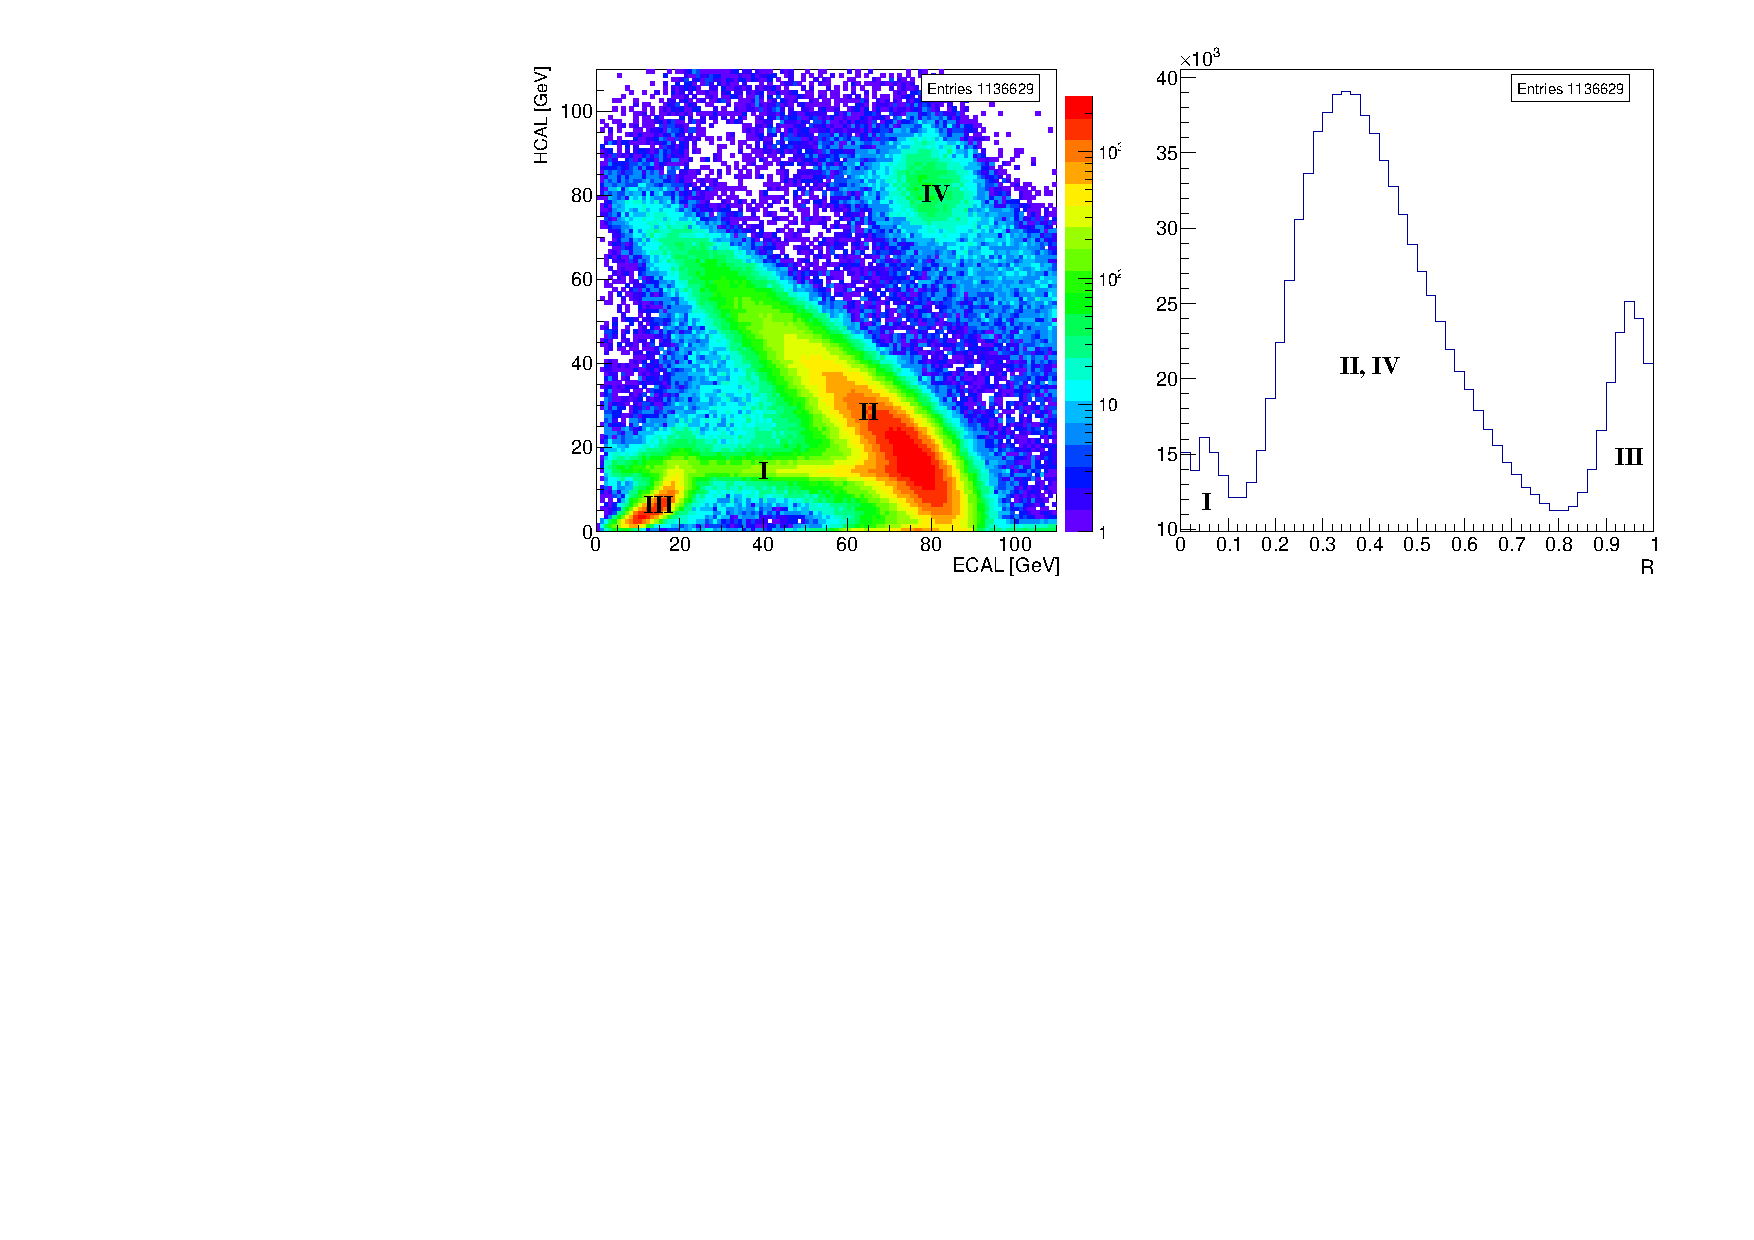
\includegraphics[width=\textwidth]{\pdirthree/pp30-calsr-uncut-may2.pdf}
  \caption[R value for control sample]{Energy distribution in the $\ehcalplane$ (left) and the corresponding distribution of the R for different interesting regions. Region I is populated by the dimuon production inside the ECAL. Region II are events leaking in the HCAL characterized by energy conservation. Region III contains events with hard bremsstrahlung of the $e^-$ upstream, where the primary completely miss the ECAL and the $\gamma$ energy is deposited in the HCAL periphery. Region IV is characterized by pileup events \cite{pdegen-thesis}.}
  \label{fig:r-value-csample}
\end{figure}

Events with electro-nuclear scattering upstream are characterized by a distribution equivalent to the one of region III. The agreement of the $R$ distribution between data and simulation was checked using data of HCAL and ECAL calibration runs, which shows a good fit with the simulated samples and small differences between different species of hadrons. This background can be suppressed by two additional tools:

\begin{itemize}
\item The straw tube in the beamline, as shown in Fig.\ref{fig:eh-prod-sketch} are in the way of the hadrons and can detect them in the periphery of their active area. A simple constraint that requires all hit to be within 3$\sigma_{beam}$ can reject this background effectively. A cut based on the multiplicity of the hit was observed to be equally powerful, since electro-nuclear interaction will produce a large number of particles in the final state \cite{pdegen-thesis}.
\item Since electronuclear interactions produce a large number of particles, this interaction saturates the MM detector strip output. A cut based on the total charge deposited in each plane is also effective to suppress the background \cite{na64-invisible-cuts}.
\end{itemize}

The first cut removed the contamination in the control sample, and where accounted for in the final background estimate. In practice, the background was extrapolated using an exponential distribution fitted using the data in the sideband C of the control sample. The results of this estimate were then accounted for conservatively in Table \ref{tab:inv-bkg}.

\begin{figure}[bht!]
  \centering
  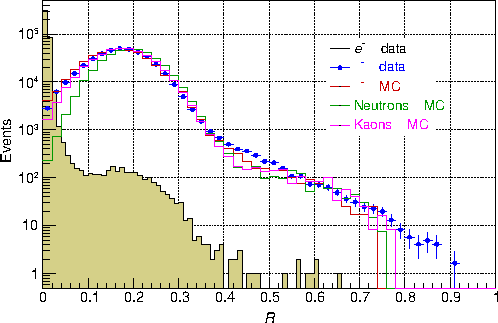
\includegraphics[width=\textwidth]{\pdirthree/HCraio-e-428-pi-3924-MC.pdf}
  \caption[R value comparison]{Distribution of the R variable for the 80 $\gev$ $e^-$, $\pi^-$, $K_L^0$ and n events obtained from data during the ECAL and HCAL calibration runs \cite{Banerjee:2020fue}.}
  \label{fig:R-comp}
\end{figure}

\begin{table}[bth!]
  \centering
  \caption[Invisible mode background]{Expected background for 2.84 $\times$ $10^{11}$ EOT collected at the time this thesis was written \cite{NA64:2019imj}}
  \begin{tabular}{lr}
    \hline \hline
    Background source & Background, $n_b$ \\
    \hline
    $\pi^-$,$\mu^-$ punchthrough                      & $<10^{-14}$ \\
    low energy $e^-$                                  & $<10^{-13}$ \\
    $e^-$/hadron nuclear interaction in target        & $<0.044$   \\
    $\pi^-$,$\mu^-$, $K_{3e}$ decay                    & 0.02 $\pm$ 0.01 \\
    $e^-$ nuclear interaction in the  beam line       & 0.43 $\pm$ 0.16 \\
    \hline
    Total (conservatively)                            & 0.53 $\pm$ 0.17 \\
    \hline \hline                       
  \end{tabular}
  \label{tab:inv-bkg}
\end{table}



\section{Visible mode analysis}
\label{ch3:sec:analysis-vis}

Similarly to the previous section, we give an overview of the selection criteria and background condition specific to the visible mode search. A new analysis I performed using the 4 GEMs tracker inside the decay volume is also described here. The validation of the MC and signal correction are done following the method described in Sec.\ref{ch3:sec:dimuons}, but also including a new tracking procedure developed to reconstruct vertex candidates in the decay volume. The background condition is similar for this analysis, as the selection criteria only differ for the low energy $\DMM$ produced in the late stage of the em-shower. A complete list of the expect background for both analyses is provided in Table \ref{tab:vis-bkg}.

\subsection{Selection criteria}
\label{ch3:sec:selection-criteria-vis}

For the visible mode, the signal is searched by matching the energy deposited in the target with the one detected by the ECAL downstream. Similarly to the invisible mode, several selection criteria ensure that the incoming particle is a well-defined electron track. Although the tracking procedure is still used to work with the control sample, the incoming particle is not required to have a momentum matching the nominal beam energy. This is because the energy conservation selection criteria already ensure that the particle will have a well-defined energy. The selection criteria for the visible mode can be summarized as follow:

\begin{itemize}
\item An energy above 1 $\mev$ is required in each SRD, and the total energy detected in both counters needs to be larger than 10 $\mev$. Events, where the energy deposit surpasses 200 $\mev$, are removed to suppress large scattering upstream or backscattering from the WCAL.
\item Energy deposit $E_{PS} > 5 \gev$ compatible with an electron in the WCAL pre-shower.
\item Energy deposited in S4 compatible with two MIP in the decay volume. This cut amounts to $E_{S_4} > $1.5$\times \emip$.
\item At least 25 $\gev$ deposited in the ECAL. This cut rejects events where low energy particle punch-through the WCAL.
\item The maximal energy of the shower should be deposited in the cell of the ECAL aligned with the beam axis (labeled as 3$\times$3). The longitudinal and lateral shape of the shower should be consistent with a single em-shower\footnote{Although the signal is expected from a $\ee$ pair, the distance of just a few $\mmi$ between the two particles does not allow for a separation between the two.}. This means a maximal energy of 3 $\gev$ is allowed in the pre-shower of the ECAL and a shower compatibility of $\chi^2 < 10$.
\item  No energy deposited in the W2 counter placed after the WCAL. The value of this cut is $E_{W2} < $0.7$\times \emip$ \cite{Banerjee:2019hmi}.  
\item Energy deposited in the VETO smaller than $E_{VETO} < 0.9\times \emip$, energy deposited in the HCAL smaller than $E_{HCAL}$1 $\gev$.  
\end{itemize}

The signal region is finally defined by looking at events where the sum of WCAL and ECAL energy is matching the nominal beam energy within the energy resolution of the detectors, i.e. $\SI{130}{\giga\electronvolt} < E_{WCAL} + E_{ECAL} < \SI{200}{\giga\electronvolt}$ (see Fig.\ref{fig:two-signature}). This energy was originally 100 $\gev$ in 2017, but was increased to 150 $\gev$ in 2018 to boost the sensitivity for short-lived $\DMX$ (see Fig.\ref{fig:w-e-vis}).

\subsection{Visible mode analysis using the tracking approach}
\label{ch3:sec:vis-mode-tracking}

The published analysis using the data collected in 2018 \cite{Banerjee:2019hmi} was based exclusively on the calorimeters and counters as described in Sec.\ref{ch2:sec:vismode}. The trackers after the decay volume were not used for signal discrimination. Here we present a novel method that exploits them providing a boost in the signal yields while maintaining the background under control. Even though this analysis is not sensitive when the decay length of the $\DMM$ is significantly smaller than the dimension of the dump, it has the advantage of being complementary to the calorimeter analysis. Unfortunately, the particularly interesting parameter space justifying the protophobic vector boson explanation of the $^8$Be anomaly is not significantly ($\lesssim$1\%) improved by this approach, the reason being the small decay length of $\DMX$ in the high-coupling region. It provides however an independent confirmation of the results obtained in \cite{Banerjee:2019hmi}, and a confirmation of the tracking procedure that be used in the next generation of this experiment (see Sec.\ref{ch5:sec:new-vismode-setup}).

While in a first approximation the $\DMM$ is produced in the first few layers of the WCAL, it can also originate at a later stage of the em-shower. These events, which are typically rejected in the calorimeter analysis, are instead accepted in the new analysis presented here. First, an initial sample is selected in the same way described above. The final discrimination in the calorimeter analysis is based on the counter W2 placed at the end of the dump to reject the charged punch-through from the em-shower. This last cut is efficient if the $\DMM$ is produced in the first few layers of the WCAL but typically rejects the event if the $\DMM$ is produced at a later stage of the em-shower. The reason is that these events are accompanied by a long longitudinal development of the em-shower that leaves an energy deposit larger than the typical energy cut accepted in the calorimeter analysis. On the other hand, the low energy of the produced $\DMM$ implies a larger angle between the decay products that can be resolved by the trackers. Combining these two concepts, one can see that the signal yield is characterized by two different topologies that can be easily distinguished by looking at the energy deposited in the ECAL (see Fig.\ref{fig:combined-analysis}).

Using this distinction, we divide all events that passed the initial selection criteria in two topologies based on the total energy deposited in the ECAL. The exact value of this threshold was selected to maximize the signal yield. The optimal value has a small dependence on the $\DMM$ mass and coupling. A simple threshold of 75 GeV amounting to half of the initial beam energy was found to be robust for most of the interesting signal scenario. After the topology is decided, a final set of cuts is applied to discriminate between signal and background. In the case of high energy $\DMM$, trackers do not have the capability of discriminating between single hits. If the energy deposited in the ECAL surpasses the 75 $\gev$, the selection criteria applied will be the one one described in the previous section. On the other hand, if the energy deposited in the ECAL is smaller than 75 GeV, trackers are used instead of the W2 as discriminator for an $\DMM$ production. Two tracks in the decay volume are required with a reconstructed vertex within 3$\sigma$ from the WCAL and an angle smaller than 3 $\mrad$. This different treatment leads to increased efficiency of the $\DMM$ produced at a late stage of the shower as shown in Fig.\ref{fig:combined-analysis}. However, the smaller energy of the $\DMM$ produced in this way has the effect of reducing the probability of the particle escaping the dump. For large coupling $\epsilon$ this suppression can be more than 2 orders of magnitude, making the boost of signal yield negligible. A summary of this boost for various interesting $\DMM$ scenario is illustrated in Table \ref{tab:dm:efftable}. The values reported consider also a conservative correction factor of 0.77$\pm$0.1 that takes into account inefficiencies of the detectors and the reconstruction algorithm. This factor was evaluated using a data-driven method precisely outlined in Sec.\ref{ch3:sec:dimuons}. We conclude that in the current setup trackers do not improve the limit on the $\DMX$ parameter space significantly. This is because the boost in signal yield becomes negligible for $\epsilon \sim 6 \times 10^{-4}$, a value which is already excluded with 90\% confidence by our previous analysis \cite{Banerjee:2019hmi}.

\begin{figure}[tbh!]
  \centering
  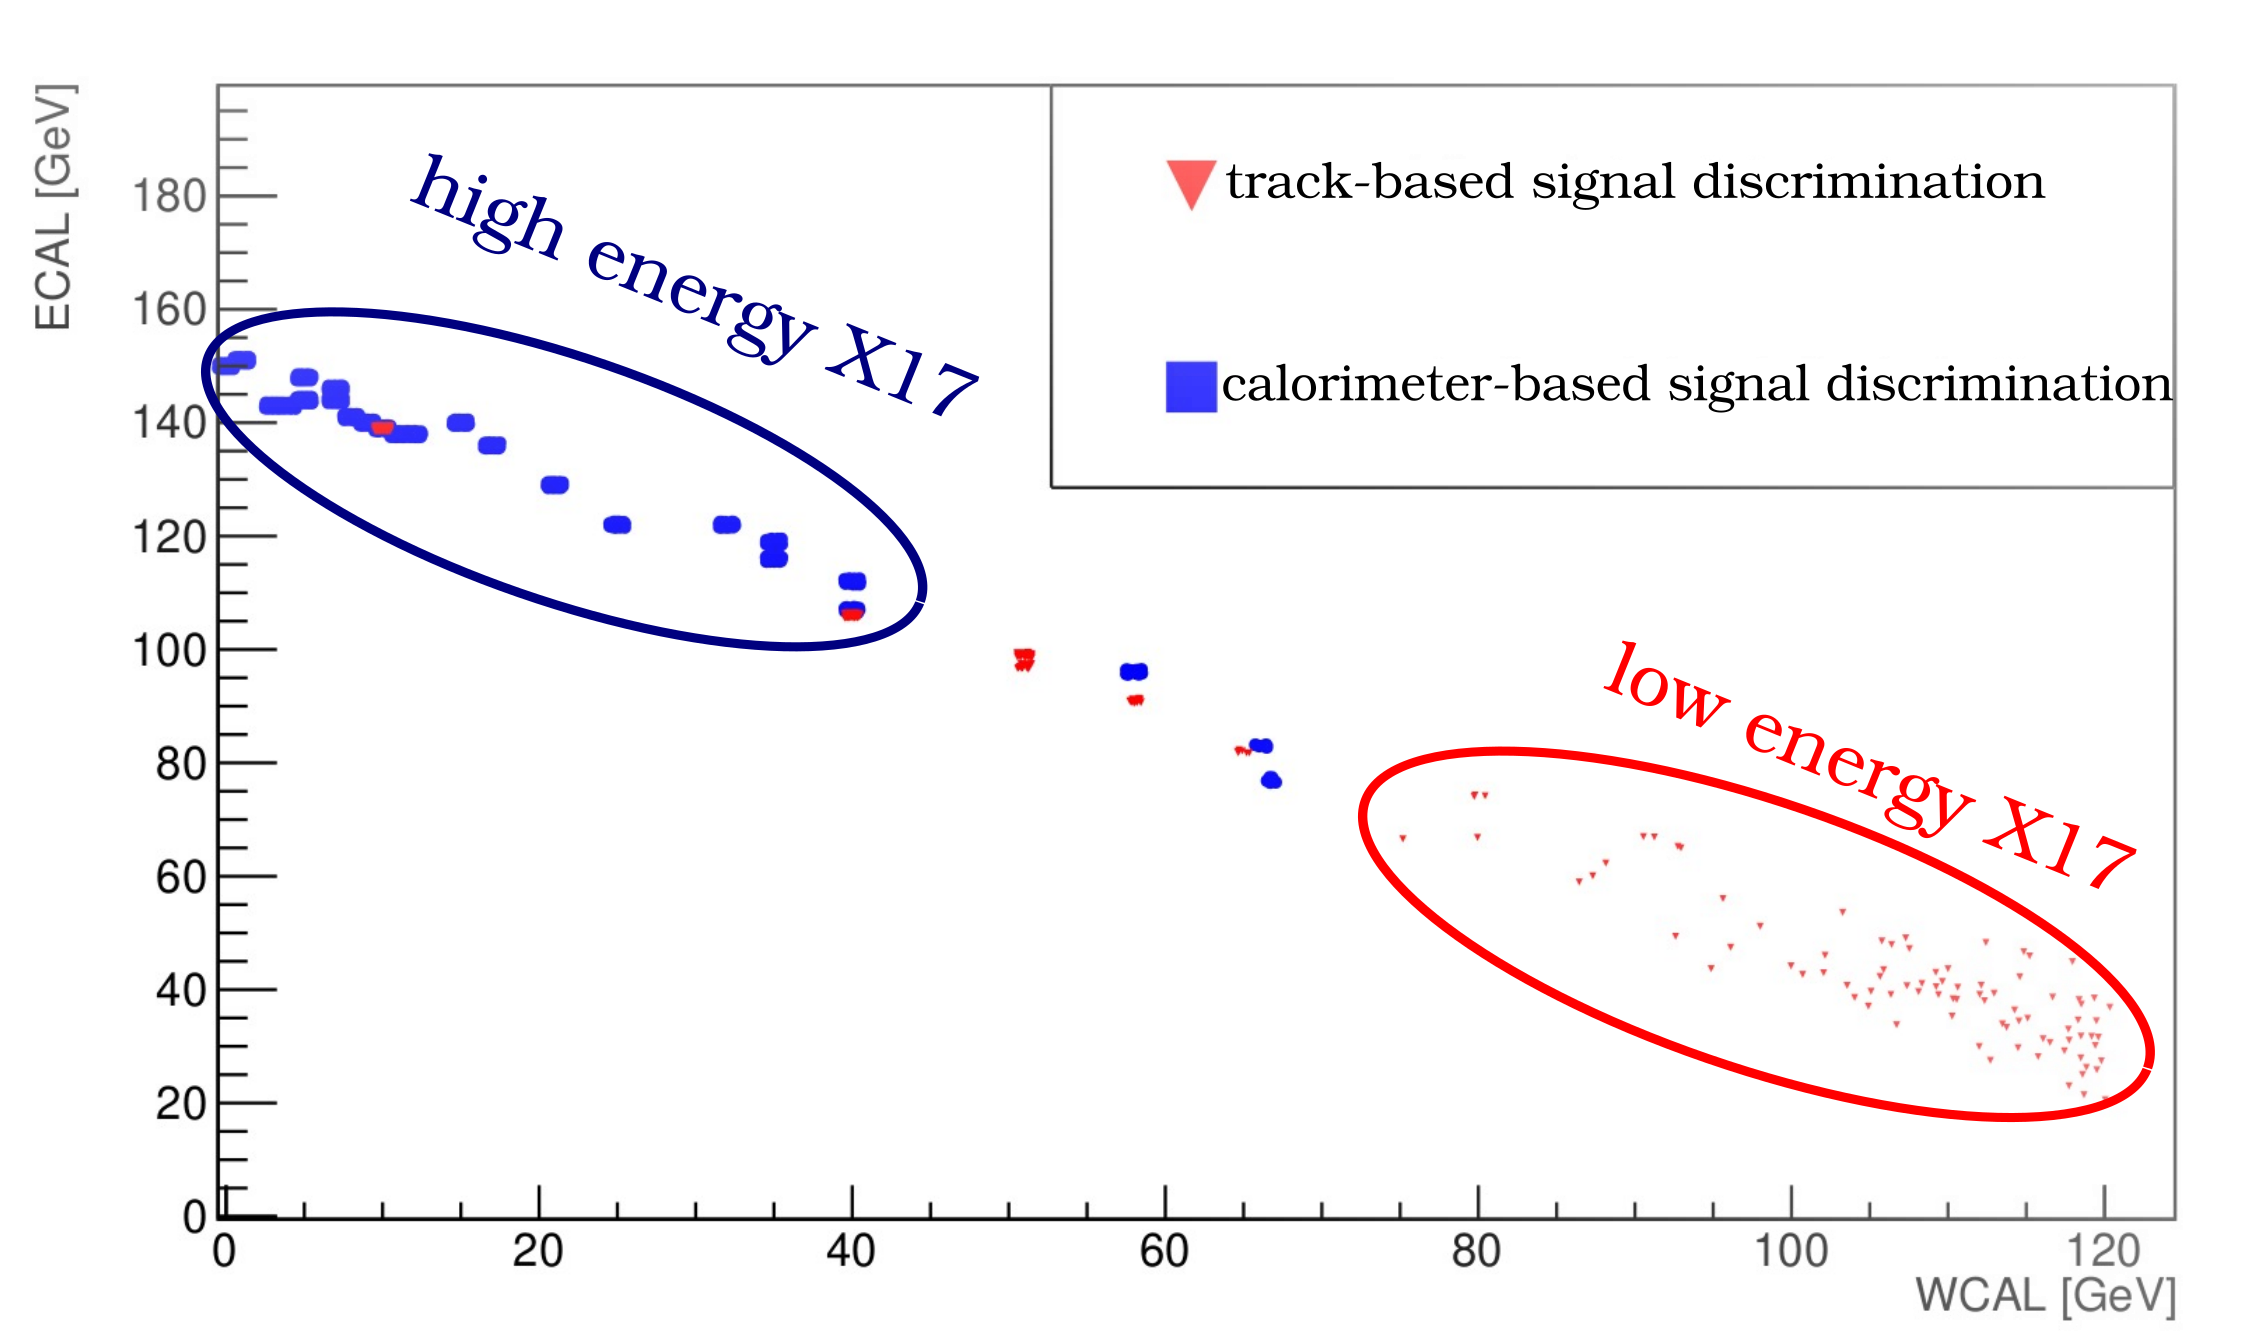
\includegraphics[width=\textwidth]{\pdirthree/X17-separation-v2.png}
  \caption[Comparison of selected $\DM$ between the calorimeter and tracking analysis]{$\DM$ simulated in the visible mode 2018 setup. Two different cuts are used to discriminate between two $\DM$ topologies. The first one is based on angle cut and vertex position using information from the 4 GEM stations installed in the decay volume and is very efficient on the $\DM$ produced at low energy (red triangle). The second one relies on the Veto placed at the end of the dump and is more efficient for the high energy population (blue square).}
  \label{fig:combined-analysis}
\end{figure}

\begin{table}[h!]
  \centering
  \begin{tabular}{|llr|}
    \hline
    M$_{A'}$ [MeV]& $\epsilon$ & N$^{new}_{A'}$ / N$^{old}_{A'}$ \\    
    \hline
    5    & 0.004    & 1   \\    
    1    & 0.0015   & 1   \\    
    1    & 0.003    & 1   \\    
    16.7 & 0.0001   & 1.22\\
    16.7 & 0.00018  & 1.2 \\    
    16.7 & 0.000316 & 1.2 \\
    16.7 & 0.0006   & 1.01\\
    16.7 & 0.0007   & 1   \\
    22   & 0.000316 & 1.22\\
    \hline    
  \end{tabular}
  \caption[ratio between signal events observed in tracker-analysis compared to calorimeter-only analysis]{N$^{new}_{A'}$ / N$^{old}_{A'}$ ratio between signal events observed in tracker-analysis compared to calorimeter-only analysis. The new analysis uses cuts based on GEM tracking detectors if the energy detected by the downstream ECAL is below 75 GeV.}
  \label{tab:dm:efftable}
\end{table}

\subsubsection{$\gamma + Z \rightarrow \mu^+ \mu^-$ events in the visible mode analysis using trackers}
\label{ch3:sec:vis-mode-tracking-dimuon}

To validate the MC simulation and the tracking procedure required for this analysis, a pure sample of events containing the rare QED interaction $\emu$ has been studied. The double tracks expected in the decay volume are then used to test the reliability of the tracking procedure in the setup. In the MC, the tracks are prepared following the procedure describe in Sec.\ref{ch3:sec:geant4-digitization} to transform the pure hits received by the MC in a common hit class that reproduces the behaviour of the GEMs detector. These tracks are then fed to the same reconstruction algorithm used for the data.

The reconstruction chain works as follows:
\begin{enumerate}
\item Track candidates are defined by grouping hits where the angle between first and second GEM pair is smaller than 9 mrad.
\item Those candidates are reconstructed using a Kalman filter implemented with the Genfit library \cite{genfit}.
\item Vertex candidates are generated by grouping tracks pair with no common hits.
\item The exact position of the vertex is obtained by back-propagating the tracks at their point of minimum distance. Only vertices with a distance below 3 $\mmi$ are considered for the analysis.
\end{enumerate}

\begin{figure}[tbh!]
  \begin{center}
    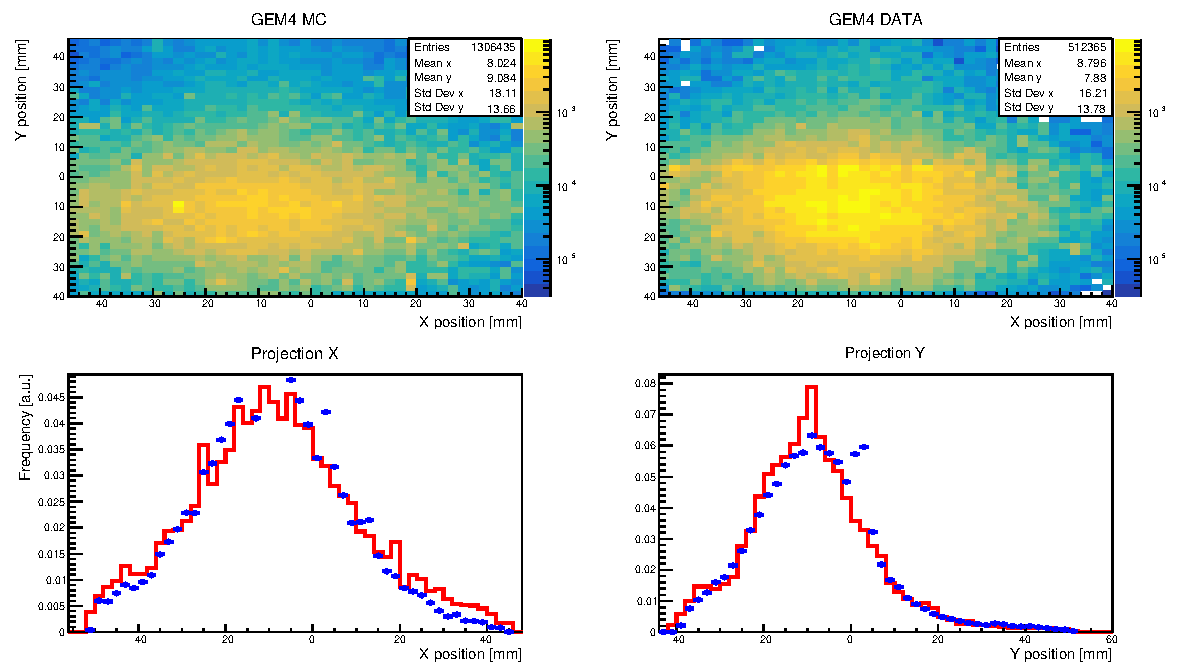
\includegraphics[scale=0.8]{\pdirthree/GEM4_rel.pdf}
  \end{center}

  \caption[Hit position of $\emu$ in GEM MC-DATA]{Hit position recorded in last GEM before ECAL for MC simulated (Red curve) and data (Blue dots) $\emu$ events.}
  \label{fig:dimuon:gemspectra}
\end{figure}
  

A dimuon sample was selected using all events collected during the visible mode 2018 run. The beam quality was improved by requiring a reconstructed momentum in the range between 140 and 160 GeV. The $\emu$ events leave a double-MIP signature in each HCAL module, thus a cut 2 GeV$<$ E$_{hcal} <$ 6.35 GeV is applied for the selection. Since the physical trigger is used during the data taking (see Sec.\ref{ch2:sec:detectors-trigger}), an additional cut $E_{WCAL} < 90$ GeV is applied to consider only such events in both simulation and data. This cut also selects a sample with kinematics closer to the one expected from a $\DM$ candidate. This makes the comparison with the MC more significant for our search. Scintillator counters also need to be compatible with a $\mu^+ \mu^-$ in the decay volume: an energy deposited of at least 1 MIP is required in the scintillator (S4) downstream the WCAL and at least 1.8 MIP in the Veto behind the ECAL. The less stringent cut on S4 is justified by its limited transverse dimension which makes it not suitable for a precise energy measurement.

Although these cuts mainly select dimuon generated from $e^-$ primaries, a contribution is also expected from the hadron contamination. The physical trigger employed in the experiment further increases such contribution, as the requirement of low energy deposit in the WCAL bias the beam composition to particles with high penetration power. To solve this issue, a cut on the SRD detector and the WCAL pre-shower are used. These cuts are expected to reject hadrons and muons at a level $\lesssim10^{-5}$.

To cross-check that the contamination is correctly removed, an independent method based on the beam profile shape is used. The beam profile significantly differs between electrons and hadrons as the H4 beamline is tuned for selecting electrons in our search. Both profiles are recovered from the data using a calibration run of electron/hadron respectively. Using a  $\chi^2$-test the ratio between the two is estimated by mixing the two templates until the best agreement with the measured beam profile is reached. The result is summarized in Fig.\ref{fig:dimuon:profile}: the beam profile of dimuon-selection events is compared before and after the SRD criteria is applied. The fit shows a contamination of roughly 50\% in the original sample. After the cut the beam profile converges to the templates obtained in the $e^-$ calibration runs.

\begin{figure}[tbh!]
  \centering
    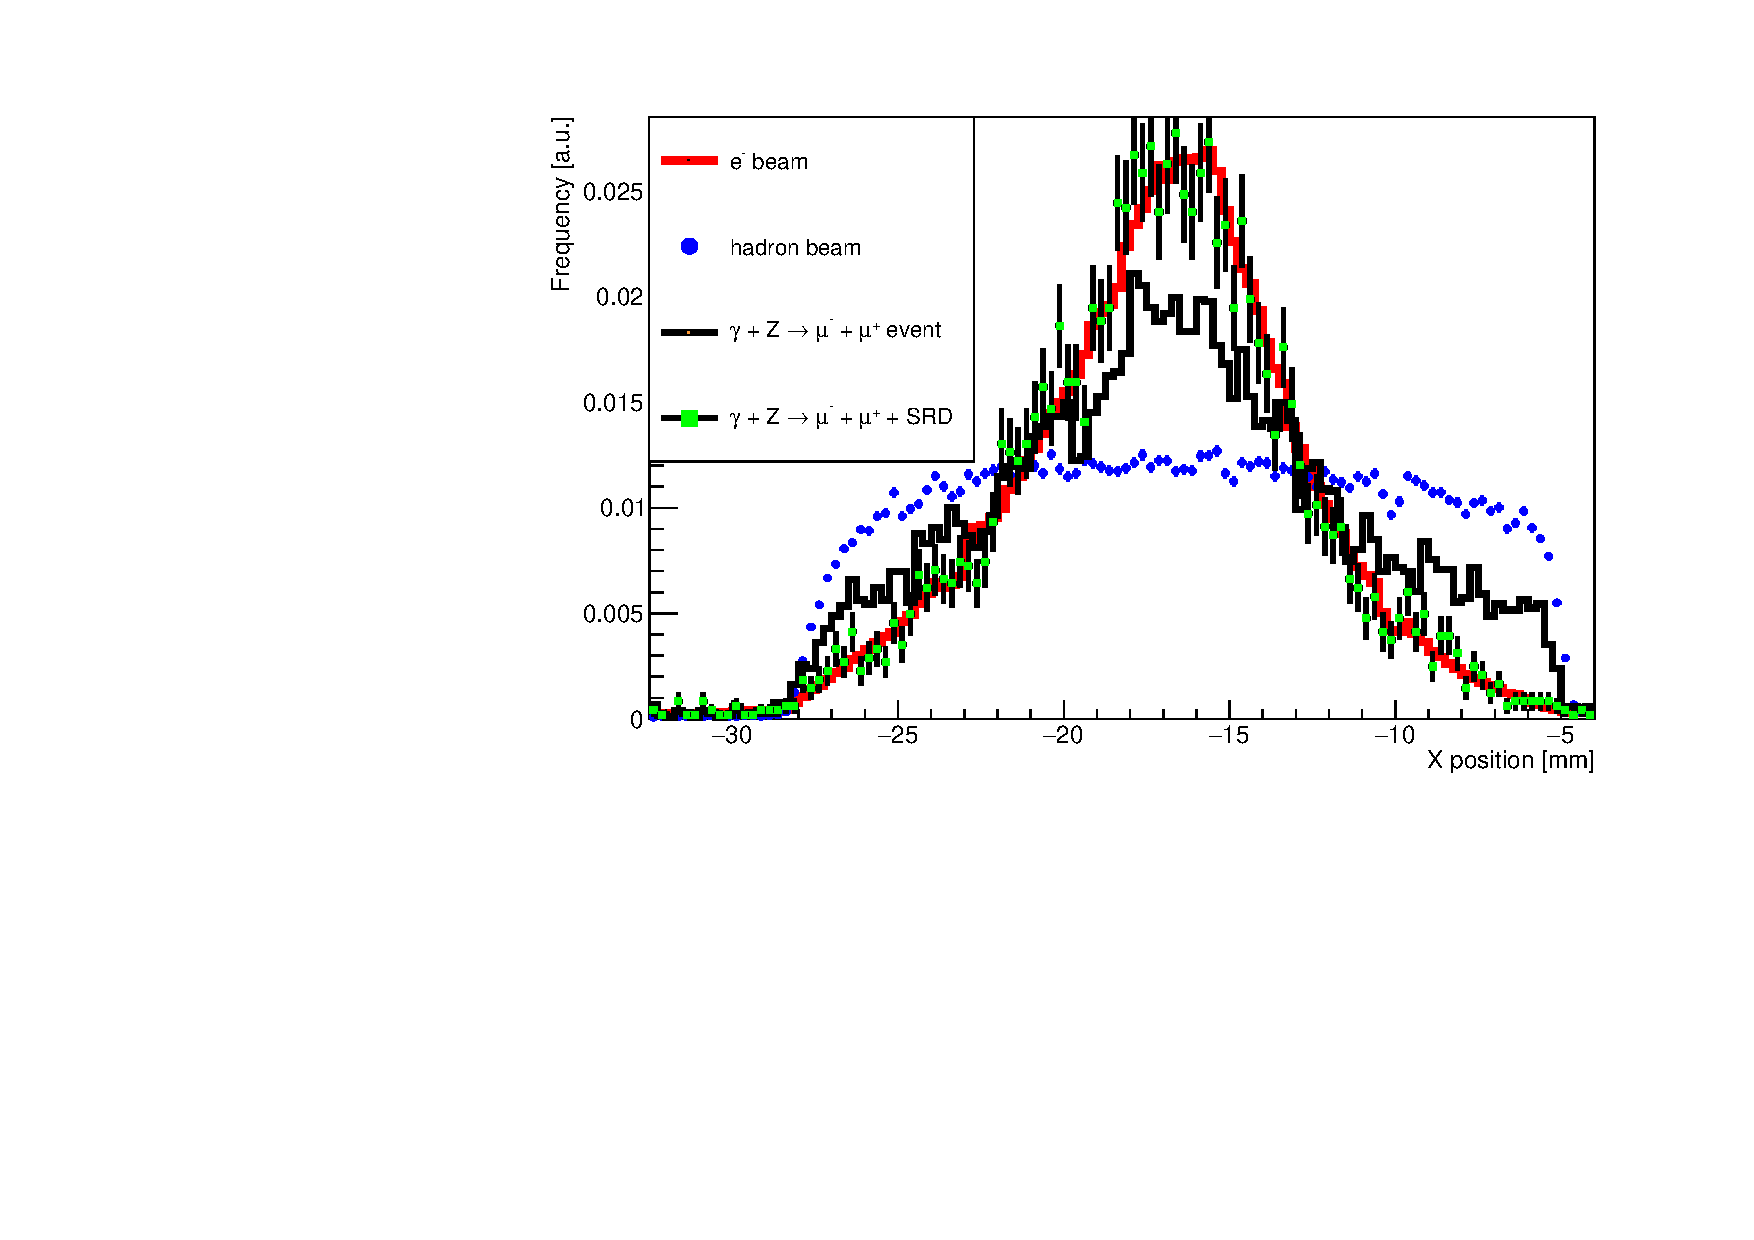
\includegraphics[width=\textwidth]{\pdirthree/beamspot.pdf}
  \caption[Beam profile with different cuts]{Beam profile recorded by the first Micromegas module upstream for hadron calibration run (blue dots), electron calibration run (red line), events selected with dimuons cuts from data collected with the physical trigger (black line) and those same events after SRD cut is applied (green square). Fits using the templates obtained from the calibration run show a level of contamination of $\sim$50\% in the dimuon sample. The contamination is completely removed after the SRD cut is applied.}
  \label{fig:dimuon:profile}
\end{figure}

%\subsection{Vertex and angle reconstruction}
%\label{ch3:sec:dimuons-reco}

\subsubsection{Signal yield correction}
\label{ch3:sec:dimuons-sig-corr}

To show that there are no significant differences in the tracking procedure between simulation and data the energy deposited in the WCAL was used as a figure of merit. If the tracking procedure affects differently data and MC, one would expect the agreement between the two distributions to diverge after cuts based on vertex reconstruction. Following the procedure described above, some vertex candidates are selected for the comparison. As the interaction $\emu$ will have their vertex inside the WCAL, only vertices compatible with this assumption are selected for the comparison. In practice, a vertex is accepted if its position lies within 3$\sigma$ of the expected WCAL position, where $\sigma$ was fitted using a Gaussian from the distribution of $\mu^- \mu^+$ pairs selected from the simulation. After the selection criteria, the energy deposited in the WCAL is compared between simulation and data for each event left (see Fig.\ref{fig:dimuon_en}). The energy deposit for data and simulation is in excellent agreement, proving that the tracking cuts do not bias the original sample.

\begin{figure}[tbh!]
  \centering
    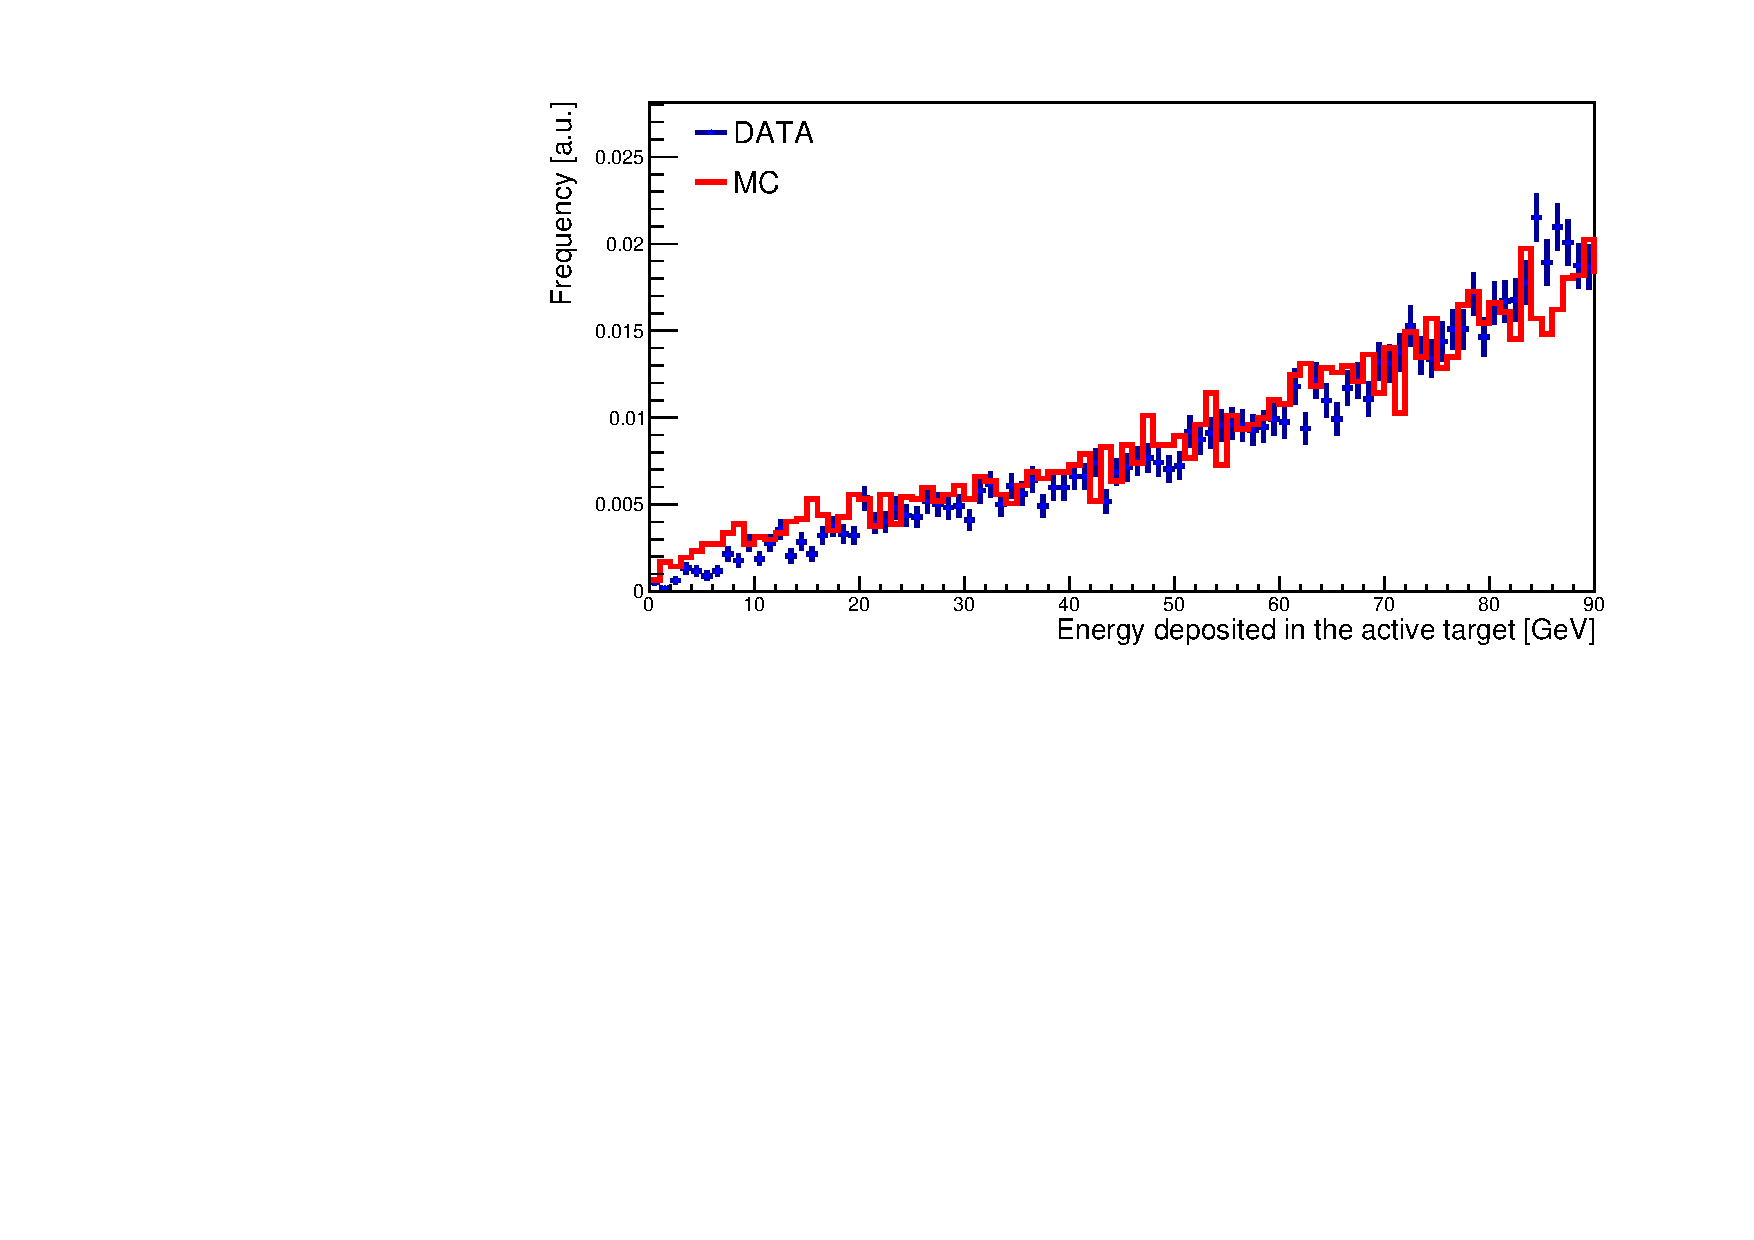
\includegraphics[width=\textwidth]{\pdirthree/dimuon_en.pdf}
  \caption[$\emu$ MC-DATA comparison in visible mode]{Energy deposit in the active dump (WCAL) after all selection criteria are applied in $\emu$ event. Data are drawn with blue dots, simulation is plotted with a red line.}
  \label{fig:dimuon_en}
\end{figure}

A lower efficiency is observed in the data compared to the Monte Carlo after applying the selection. The reasons for this are inefficiency of the GEM modules, fail of clusterization in some events and differences in the tracking procedure due to the simplifications used in the MC. The cuts applied to the sample are divided into four steps. First, at least two hits per GEM are required in the decay volume as a minimal condition for tracking. After that, events with a GEM module recording more than 5 hits are rejected as incompatible with a single $\emu$ vertex. The MC predicts 68\% of $\mu^+ \mu^-$ pair after these two cuts. This low acceptance is caused by the GEMs position optimized to resolve very close hits coming from the decay of $\DM$. These selection criteria do not depend on the track-fitting procedure but instead rely on the clusterization performed and the efficiency of the trackers. Tracking procedure is then applied to the events that survived the two first requirements. The reconstructed vertex position is required to be compatible with a vertex inside the dump. The number of events surviving the last requirement  is slightly smaller in the data. The disagreement between the ratio of good vertices reconstructed inside the decay volume is $<$1\%. A total factor of 0.77 is estimated as ratio between data and MC. This factor is used to correct the 2018 signal yield. A summary of the efficiency can be found in Table \ref{tab:dimuon:efficiencies}.

\begin{center}
\begin{table}
  %\centering
  \begin{tabular}{|l|c|c|c|}
    \hline
    cut & efficiency MC & efficiency Data & MC / DATA \\
    \hline
    \multicolumn{4}{|l|}{\textbf{Hit}}\\
    \hline
    hits per GEM $\geq$ 2 & 0.68$\pm$0.1 & 0.58$\pm$0.1 & 0.85$\pm$0.1 \\
    hits per GEM $\leq$ 5 & 0.68$\pm$0.1 & 0.55$\pm$0.1 & 0.80$\pm$0.1 \\
    \hline
    \multicolumn{4}{|l|}{\textbf{Tracking}}\\    
    \hline
    Vertex distance $\leq$ 3 $\mmi$ & 0.63$\pm$0.1 & 0.49$\pm$0.1 & 0.77$\pm$0.1  \\
    Vertex in decay volume & 0.62$\pm$0.1 & 0.48$\pm$0.1 & \textbf{0.77$\pm$0.1}\\
    \hline
    
  \end{tabular}
  \caption[MC/DATA for the tracking procedure and vertex reconstruction]{Efficiency of cuts based on tracking criteria for a clean sample of simulated $\emu$ and dimuon selected from 2018 data. The efficiency presented in the table are cumulative, with the first cut applied being the one in the first row. First two cuts are based exclusively on information coming from the single GEM modules. Last two cuts are based on the tracking procedure.}
  \label{tab:dimuon:efficiencies}
\end{table}
\end{center}

\subsection{Background}
\label{ch3:sec:bkg:vis}

Since the analysis requires the sum of the energy deposited in the two calorimeters (WCAL and ECAL) to be equal to the incoming primary energy, particles escaping the setup in the transverse direction are no longer a source of background as in the invisible mode. Because of the large distance between the WCAL and ECAL\footnote{7.5 \si{\meter} in the 2018 setup, 4.2 \si{\meter} in the 2017 setup}, such event is actually frequently observed. The background, on the other hand, can be caused by particles able to punch-through the first target without leaving any energy deposit in the W2 counter and then leave a pure electromagnetic signature in the ECAL downstream. Because of the different lengths of the setup and the addition of a vacuum tube (see Fig.\ref{fig:setup-vis-2018}), the background calculated for 2017 and 2018 differs significantly. The exact suppression depends on the exact source of background considered, but it can amount up to one order of magnitude \cite{Banerjee:2019hmi}. This thesis presents an alternative approach to \cite{Banerjee:2019hmi} that relies on the GEM trackers to boost the signal yield. The background condition do not differ significantly and are reported in Table \ref{tab:vis-bkg}


\subsubsection{Hadronic background}
\label{ch3:sec:bkg:vis:hadr}

Starting from the most simple scenario, punch-through of $\pi^-$ can be background if no energy is deposited in the W2 counter, an energy $> 2\emip$ in S4 is deposited, and the particle deposit the rest of its energy in the ECAL. The product of these probabilities was conservatively estimated to be $< 10^{-12}$ when factoring SRD and HCAL suppression.

Inelastic scattering in the WCAL, for example in the form of

\begin{equation}
  \label{eq:vis-int-neutral}
  \pi^- + p \rightarrow (\geq 1)\pi^0 + (neutrals)
\end{equation}

can be a source of background as they can punch-through the W2 undetected. This was estimated using the extrapolation of the charge-exchange cross-section, measured on different nuclei, after taking into account SRD rejection. In the tracking-analysis, inelastic scattering in the WCAL produces a large occupancy in the decay volume that can potentially create vertex candidates. Such events are expected to be suppressed by the selection criteria applied downstream for hadron rejection outlined in Sec.\ref{ch3:sec:selection-criteria-vis}. Furthermore, events able to mimic the pure electromagnetic signal of the decay $\DM \rightarrow e^+ e^-$ are often accompanied by a large transversal spread and are thus rejected by the requirement of energy conservation at a level of $\lesssim 10^{-5}$. This estimate was obtained by integrating the events in the signal region with two tracks in the decay volume without applying any rejection criteria for hadrons in a $\pi^-$ simulation. Such an event should also pass the independent selection criteria applied upstream, namely large energy deposited in the SRD and WCAL pre-shower. In a sample up to $10^7$ EOT, it was not possible to find an event with such signature even after removing the HCAL and VETO from the selection criteria.

To estimate the background for a larger number of EOT, the $\ks$ decay was used as a benchmark process, as its short decay length is expected to be compatible with the ones of the $\DM$. The energy spectrum of $\ks$ was simulated using an exponential distribution with an energy cut-off of 18 GeV, as $\ks$ below this energy has a negligible probability to decay outside the dump. To estimate the number of $\ks$ in the sample, events with a punch-through neutral were selected by applying all selection criteria to the control sample but changing the requirement for $S_4$ to $E_{S_4} < 0.5 \emip$. The distribution of these events is shown in Fig.\ref{fig:w-e-vis}. Here we label signal-like the events that passed all selection criteria in the control sample. One such event was recorded in 2017, well outside of the signal region. In 2018 the number of neutral was reduced by a factor 2-3, and no signal-like events were observed. These data were used to estimate the ratio between neutral and signal-like events using the MC-simulation of $\ks$. This resulted in an estimate of 0.06 events for the 2017 data and 0.005 events for 2018 data. The statistical fluctuation of the data dominates the error for this estimate.

To estimate the background for the tracking analysis, tracking-criteria were applied over the $\ks$ MC-sample. It was estimated that a rejection of $10^{-2}$ can be conservatively achieved for this background using the opening angle of the reconstructed vertex as a discriminator. This estimate however mostly depends on the main hadronic decay channel $\ks \rightarrow \pi^- + \pi^+$ which is further suppressed downstream by the hadron suppression cuts such as no energy deposited in the HCAL and the VETO. The decay channel $K^0_S \rightarrow \pi^0 + \pi^0$ has on the other hand a small chance to leave any signature in the GEM modules as no charged particle is typically emitted. Signal-like events can be produced either by the conversion of a photon from the $\pi^0 \rightarrow \gamma \gamma$ decay into a $\pair$ pair or in the decay chain $\ks \rightarrow \pi^0 + \pi^0 (\pi^0 \rightarrow \gamma + e^- + e^+$). This last channel is however suppressed by its low branching ratio $\Gamma_i$/$\Gamma \approx $1\% \cite{review-particle-physics}. A dedicated simulation performed with a biased branching ratio shows that the rejection for this channel is further improved to $\lesssim 10^{-3}$ since the large emission angle of a three-body decay is significantly different from the one expected in the $\xdecay$ decay. A conservative rejection of $\lesssim 10^{-5}$ is reached accounting both suppression factors. If we add the suppression factor coming from the angle using the trackers to what was computed for the calorimeter-analysis, one can conservatively estimate the background contribution from $\ks$ to be at a level of $<0.001$.


\begin{figure}[bth!]
  \centering
  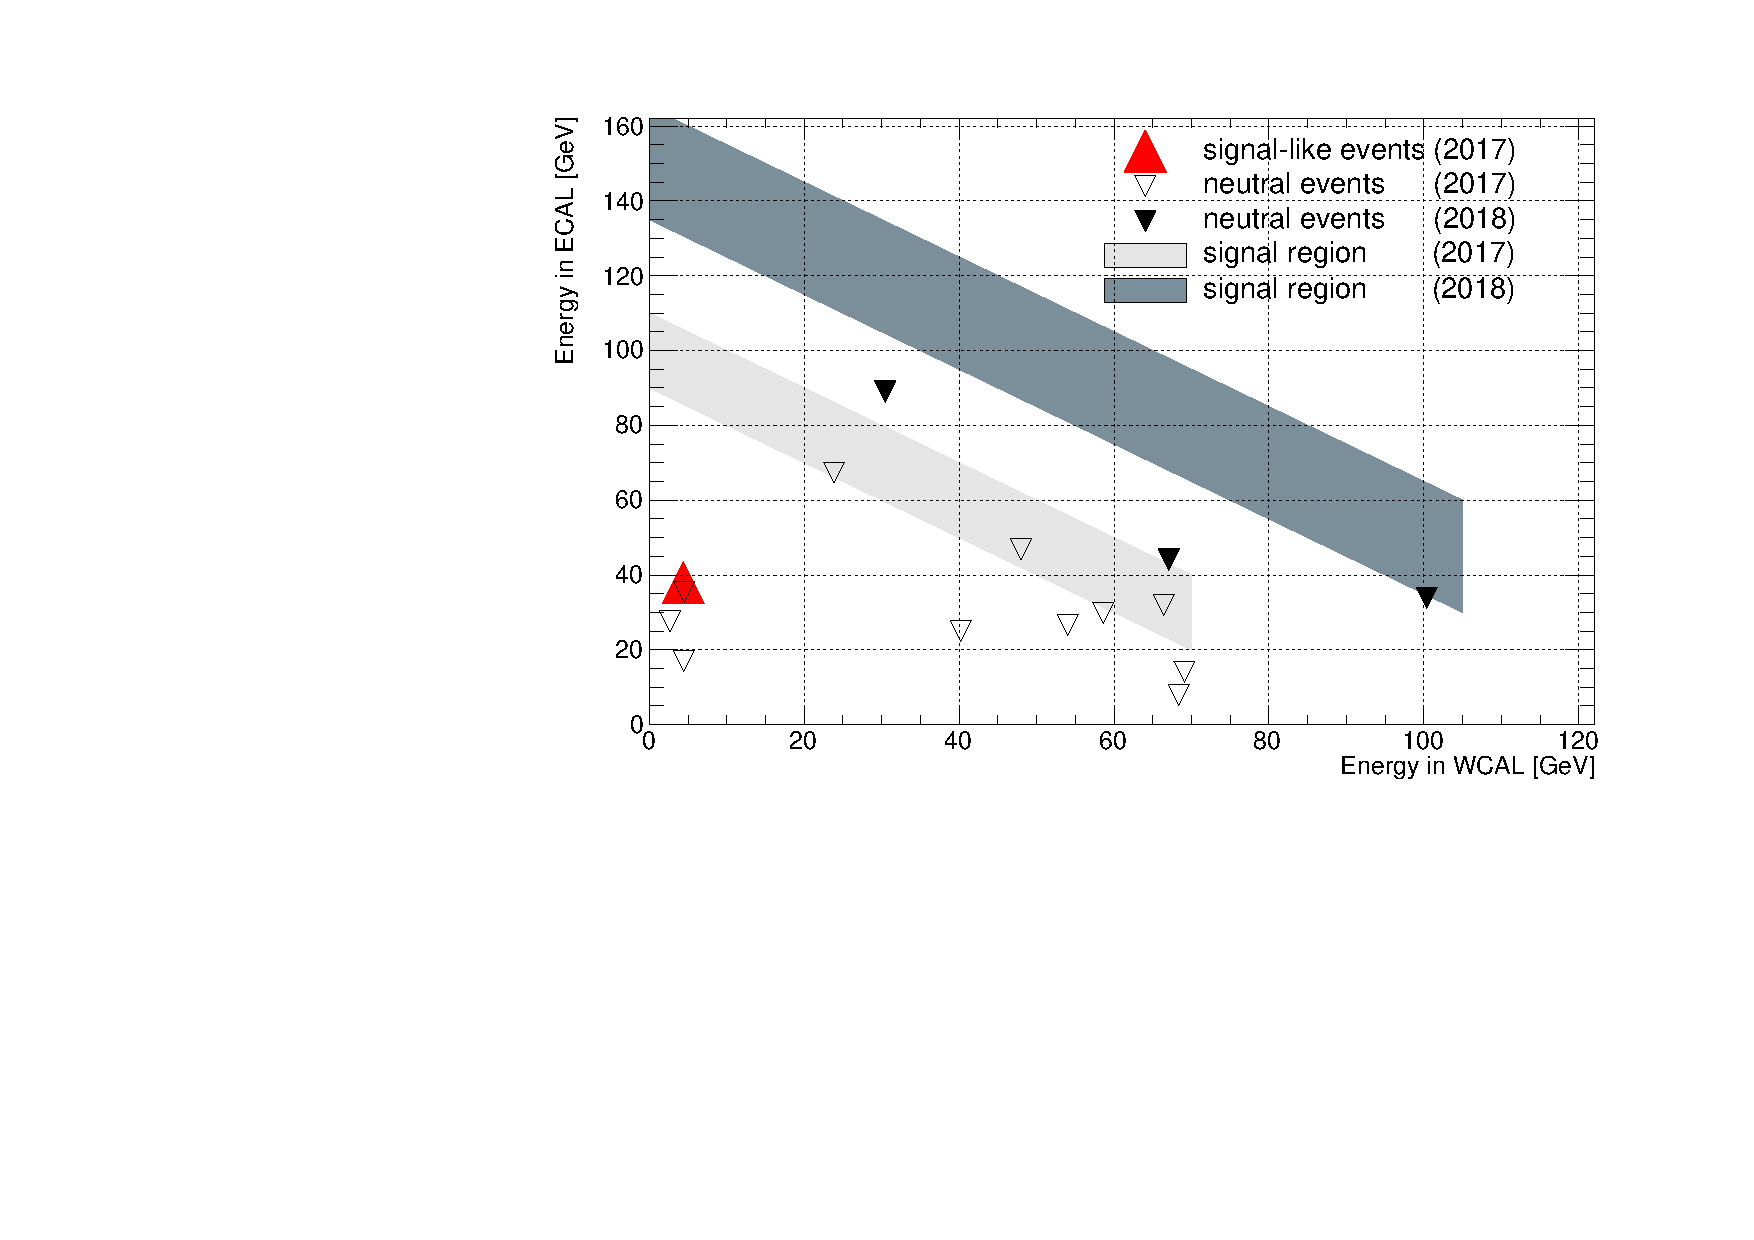
\includegraphics[width=\textwidth]{\pdirthree/w-e-neutrals.pdf}
  \caption[neutral events in visible mode]{Distribution of selected signal-like events in the $\ehcalplane$ plane for 2017 and 2018 data. Neutral events are shown as hollow (2017) and full (2018) triangles. The two shadowed bands represent the signal box region for the two different runs. A single signal-like event detected during the 2017 run not falling into the signal region is shown with a red triangle \cite{Banerjee:2019hmi}.}
  \label{fig:w-e-vis}
\end{figure}

\subsubsection{Muonic background}
\label{ch3:sec:bkg:vis:muon}

Background coming from $\mu^-$ primaries is very suppressed for the visible mode and is dominated by the probability of punch-through $\mu^-$ that leaves most of its energy inside the ECAL. This is similar to a $\pi^-$ punch-through, with the difference that the probability of it happening is lower due to both beam suppression and the absence of strong interaction. The background can be conservatively estimated to be $<10^{-14}$.

\subsubsection{Electronic background}
\label{ch3:sec:bkg:vis:elec}

The main contribution of the background from $e^-$ primary is the punch-through of high-energetic $\gamma$ that converts on the last tile of the WCAL or some material downstream and produces an $\ee$ pair. Since this background depends on the longitudinal fluctuation of the em-shower, it is hard to predict using MC-simulations alone. To estimate such contribution for $\sim10^{11}$ EOTs a data-driven method is used. A sample of 3$\cdot 10^9$ EOT was considered, roughly corresponding to $\sim$10\% of the data collected in 2018. Events in the signal region with $E_{ECAL} < 105$ GeV were selected with the requirement of at least two hits in each GEM module. Only one event with such property was found. Assuming a suppression due to the angle and minimal vertex requirement of $10^{-3}$ or $S_4$ selection criteria this would push our background down conservatively to a level $<10^{-13}$. The analysis of the full 2018 data is compatible with this estimate: a total of three events were found with 2 two hits in the GEM modules. For none of these events it was possible to reconstruct a physical vertex, suggesting that these particles experienced large multiple-scattering inside the WCAL before reaching the GEMs.


\begin{table}[bth!]
  \centering
  \caption[Visible mode background]{Expected background for 5.5$\times$ $10^{10}$ EOT collected in 2017 \cite{Banerjee:2018vgk} and the 3.3$\times$ $10^{10}$ EOT collected in 2018 \cite{Banerjee:2019hmi}. The third column shows background for 2018 including the GEM trackers in the analysis.}
  \begin{tabular}{lrrr}
    \hline \hline
    Background source                           & $n_b$ (2017)      &  $n_b$ (2018)   & $n_b$ (2018, new analysis)\\
    \hline
    $\pi^-$ punch-through                        & 0.0015$\pm$0.0008 &  0.0007$\pm$0.0004   & 0.0007$\pm$0.0004   \\    
    $\ks \rightarrow \pi^0 \pi^0$                     & 0.06$\pm$0.034    & 0.005$\pm$0.003 &     $<$0.001\\
    $e^-$/hadron nuclear interaction  & 0.01$\pm$0.004    & 0.01$\pm$0.004  & 0.01$\pm$0.004\\    
    $\mu^-$ punch-through                        & $<0.001$ & $<0.001$ & $<0.001$       \\            
    $\pi^-$,$K^- \rightarrow e\nu$ $K_{4e}$              & $<$0.001 & $<0.001$ & $<0.001$\\
    $eZ \rightarrow e Z \mu^+\mu^-;\mu^{\pm}\rightarrow e^{\pm}\nu\bar{\nu}$ & $<$0.001 & $<0.001$ & $<0.001$\\
    punch-through $\gamma$ & $<$0.001 & $<$0.0005 & $<$0.001 \\
    \hline
    Total (conservatively)                      & 0.07 $\pm$ 0.035   & 0.006 $\pm$ 0.003  & 0.006 $\pm$ 0.003\\
    \hline \hline                       
  \end{tabular}
  \label{tab:vis-bkg}
\end{table}

%%% Local Variables:
%%% mode: latex
%%% TeX-master: "../PhDthesis"
%%% End:
